
%%%%%%%%%%%%%%%%%%%%%%%%%%%%%%%%%%%%%%%%%%%%%%%%%%%%%%%%%%%%%%%%%%%%%%%%%%%
%DO NOT MAKE CHANGES IN THIS FILE

\documentclass[12pt, a4paper]{report}
\usepackage[left = 1.5in, right = 1in, top = 1in, bottom = 1in]{geometry}%for margin
\usepackage{amsfonts, amsmath, amssymb} %for mathematical equations
\usepackage{graphicx} %for images

\usepackage{times} %font Times New Roman Font
\usepackage{float} %required if you use H(strictly here) position for floats
\usepackage[skip = 8pt,tableposition=top, figureposition=bottom]{caption}%adjust spacing of captions and specify where captions are
\usepackage{hyperref} % for easy Navigation in document, also puts links in TOC, LOF, LOT...
\usepackage{setspace} %to change line spacing in some portion \singlespacing \onehalfspacing \doublespacing
\usepackage{acro} %for List of Abbrreviation and Symbol
\acsetup{first-style = short} % set to display only short form on the command \ac{}

%packages required for complex tables
\usepackage{bigstrut} 
\usepackage{multirow}
%package for greek letters
\usepackage[euler]{textgreek}
\renewcommand{\contentsname}{Table of Contents} %Change TOC Heading ... default is "Contents" 

\parindent 0pt	%removes the indent in paragraph
\setlength{\parskip}{18pt}	%for paragraph spacing
\renewcommand{\baselinestretch}{1.5}   %Line Spacing = 1.5 line-spaces

%to reduce spacing in sections
\usepackage{titlesec}
\titlespacing*{\section}{0pt}{0pt}{0pt} %left, top, bottom spacings
\titlespacing*{\subsection}{0pt}{0pt}{0pt}
\titlespacing*{\subsubsection}{0pt}{0pt}{0pt}
\titlespacing*{\paragraph}{0pt}{0pt}{0pt}
\titlespacing*{\subparagraph}{0pt}{0pt}{0pt}

%adjust fontsizes\ of sections
\titleformat*{\section}{\fontsize{14pt}{18pt}\bfseries}
\titleformat*{\subsection}{\fontsize{13pt}{18pt}\bfseries}
\titleformat*{\subsubsection}{\fontsize{12pt}{18pt}\bfseries}
\titleformat*{\paragraph}{\fontsize{12pt}{18pt}\bfseries}
\titleformat*{\subparagraph}{\fontsize{12pt}{18pt}\bfseries}

%to reduce separation between points in list
\usepackage{enumitem}
\setlist[enumerate]{nosep} % no separation between items in enumerate
\setlist[itemize]{nosep} % no separation between items in itemize
%use \vspace{-18pt} before list to reduce paragraph spacing between list and preceeding paragraph.

%Changes for Chapter Heading Spacing and formats for numbered chapters
\makeatletter
\def\@makechapterhead#1{%
  %\vspace*{50pt}%
  {  \MakeUppercase{\ifnum \c@secnumdepth >\m@ne
        \fontsize{16pt}{1}\bfseries \@chapapp \space \thechapter\vspace{5pt}\\
    \fi
    \interlinepenalty\@M
     \bfseries #1}\par\nobreak
    %\vskip 0pt
  }}
\makeatother

%%%%%%%%%%%%%%%%%%%%%%%%%%%%%%%%%%%%%%%%%%%%%%%%%%%%%%%%%%%
%to adjust Heading spacings and fonts For unnumbered chapters, TOC, LOF ...
\makeatletter
% Redefine the \chapter* header macro to remove vertical space
\def\@makeschapterhead#1{%
  %\vspace*{50\p@}% Remove the vertical space
  {\newpage \parindent \z@ \raggedright
    \normalfont
    \interlinepenalty\@M
    \center \fontsize{16pt}{1} \bfseries \MakeUppercase{#1}\par\nobreak
    %\vskip 18\p@ % adjust space after heading 18pt
  }}
\makeatother 
%%%%%%%%%%%%%%%%%%%%%%%%%%%%%%%%%%%%%%%%%%%%%%%%%%%%%%%%%%%

%%%%%%%%%%%%%%%%%%%%%%%%%%%%%%%%%%%%%%%%%%%%%%%%%%%%%%%%%%%%%%%%%%%%%%%%%%%
% newcommand for generating Cover Page
\newcommand{\KECcoverpage}
{
\begin{titlepage}
\begin{center}
\Large{\textbf{KANTIPUR ENGINEERING COLLEGE}}\\
\large{\textbf{(Affiliated to Tribhuvan University)}}\\
\large{\textbf{Dhapakhel, Lalitpur}}\\
\vfill	%vertically fill the space 
\begin{figure}[h] % h: put logo "here"
\begin{center}

\includegraphics[width=25mm, height = 25mm]{images/logo.png}
\end{center}
\end{figure}

\large{\textbf{[Subject Code: \subCode]}}\\ %Chcite handeu ta iza}ange This Line
\large{\textbf{A \MakeUppercase{\project} \MakeUppercase{\doc} ON}}\\ %Change This Line
\Large{\textbf{\MakeUppercase{\projectTitle}}}\\

\vfill	%vertically fill the space 
\large{\textbf{Submitted by:}}\\
\large{\textbf{\submittedBy}}\\
\vfill	%vertically fill the space 
\textbf{A \MakeUppercase{\project} SUBMITTED IN PARTIAL FULFILLMENT OF THE REQUIREMENT FOR THE DEGREE OF \MakeUppercase{\degree}}\\

\vfill	%vertically fill the space 
\large{\textbf{Submitted to:}}\\
\large{\textbf{\submittedTo}}\\
\vfill
\large{\textbf{\defDay\ \defMonth, \defYear}}
\pagebreak
\end{center}
\end{titlepage}
}
%%%%%%%%%%%%%%%%%%%%%%%%%%%%%%%%%%%%%%%%%%%%%%%%%%%%%%%%%%%%%%%%%%%%%%%
% newcommand for generating Cover Page
%Title Page
\newcommand{\KECtitlepage}
{
\begin{titlepage}
\begin{center}
\Large{\textbf{\MakeUppercase{\projectTitle}}}\\

\vfill	%vertically fill the space 

\large{\textbf{Submitted by:}}\\
\large{\textbf{\submittedBy}}\\

\if{\ne{\supervisor}{none}} \\ Displays Supervisor name only if it is not "none"
	\vfill	%vertically fill the space 
	\large{\textbf{Supervised by:}}\\
	\large{\textbf{\supervisor}}\\
	\large{\textbf{\degSup}}\\
\fi
\vfill	%vertically fill the space 
\textbf{A \MakeUppercase{\project} SUBMITTED IN PARTIAL FULFILLMENT OF THE REQUIREMENT FOR THE DEGREE OF \MakeUppercase{\degree}}\\

\vfill	%vertically fill the space 
\large{\textbf{Submitted to:}}\\
\large{\textbf{\submittedTo}}\\
\large{\textbf{Kantipur Engineering College}}\\
\large{\textbf{Dhapakhel, Lalitpur}}\\

\vfill
\large{\textbf{\defDay\ \defMonth, \defYear}}
\thispagestyle{empty}\\ %to remove page number
\pagebreak
\end{center}
\end{titlepage}
}
%%%%%%%%%%%%%%%%%%%%%%%%%%%%%%%%%%%%%%%%%%%%%%%%%%%%%%%%%%%%%%%%%%%%%%
%command for copyright page
\newcommand{\KECcopyright}
{
\chapter*{Copyright}%Required only for Final Defense of Major Project
\addcontentsline{toc}{chapter}{Copyright}
The author has agreed that the library, Kantipur Engineering Collage, may make this report freely available for inspection. Moreover the author has agreed that permission for extensive copying of this report for scholarly purpose may be granted by the supervisor(s), who supervised the project work recorded herein or, in their absence, by the Head of the Department wherein this project was done. It is understood that due recognition will be given to the author of this report and to the \submittedTo, Kantipur Engineering College in any use of the material of this report. Copying or publication or other use of this report for financial gain without approval of the \submittedTo, Kantipur Engineering College and author’s written permission is prohibited.\par Request for permission to copy or to make any other use of the material in this report in whole or in part should be addressed to:

Head\\
\submittedTo\\
Kantipur Engineering College\\
Dhapakhel, Lalitpur\\
Nepal
}
%%%%%%%%%%%%%%%%%%%%%%%%%%%%%%%%%%%%%%%%%%%%%%%%%%%%%%%%%%%%%%%%%%%%%%
%command for Approval Letter
\newcommand{\KECapproval}
{
\chapter*{Kantipur Engineering College
\vskip -10pt}%Required only for Final Defense of Major Project
\begin{center}
\fontsize{12.8pt}{1} %size decreaced to adjust department name in single line
\textbf{
\MakeUppercase{\submittedTo}\\ %for department name
}
\vskip 10pt
\fontsize{16pt}{1}
\textbf{APPROVAL LETTER}
\end{center}
\vskip -16pt
\addcontentsline{toc}{chapter}{Approval Letter}%
The undersigned certify that they have read and recommended to the Institute of Engineering for acceptance, a project report entitled "\projectTitle " submitted by \\
\submittedBy \\
in partial fulfillment for the degree of \degree. \par
{\vspace{25pt}
..........................................\\
Supervisor\\
\supervisor \\
\degSup\\
\vspace{25pt}\\
..........................................\\
External Examiner\\
\external\\
\degExternal\\
\vspace{25pt}\\
..........................................\\
\hod\\
Head of Department\\
\submittedTo
\vspace{10pt}\\
Date: \defMonth\space\defDay ,\space \defYear
\singlespacing\par
} %single spacing for the texts inside {}
}

%command for list of abbreviations
\newcommand{\KECloa}
{
%\chapter*{List of Abbreviations}
\addcontentsline{toc}{chapter}{List of Abbreviations}
\vskip -42pt % to reduce space due to invisivle acronym class name
{
\singlespacing
\printacronyms[include-classes=abbr, name= List of Abbreviations ]
}

}

%command for list of symbols
\newcommand{\KEClos}
{
\chapter*{List of Symbols}
\addcontentsline{toc}{chapter}{List of Symbols}
\vskip -42pt % to reduce space due to invisivle acronym class name{
{
\singlespacing
}
}

%command to adjust toc, lof, lot spacing
\newcommand{\KECadjusttocspacings}
{
\parskip 0pt % to remove paragraph spacing in TOC, LOF ...
\renewcommand{\baselinestretch}{0.1} % to adjust line spacing in toc
\newcommand*{\noaddvspace}{\renewcommand*{\addvspace}[1]{}}
\addtocontents{lof}{\protect\noaddvspace} %remove extra vertical space in LOF
\addtocontents{lot}{\protect\noaddvspace} %remove extra vertical space in LOT
}

 %includes the file KecReportFormat.tex that include all  necessary formattings
\usepackage{amsmath}
\usepackage{algorithm}
\usepackage{algorithmic}
%%%%%%%%%%%%%%%%%%%%%%%%%%%%%%%%%%%%%%%%%%%%%%%%%%%%%%%%%%%%%%%%%%%%%%%%%%%
%Define Macros for Details of your Project
\newcommand{\project}{Major Project } %Specify "Major Project" or "Minor Project"
\newcommand{\projectTitle}{FEATHERFIND : BIRD SPECIES IDENTIFICATION FROM AUDIO} %specify "Title" of Your Project
\newcommand{\doc}{Mid-Term Report} % specify the document you are preparing eg. "Proposal", "Mid-Term Report" or "Final Report"32
% Note that You have to sibmit "Final Report" for Pre-final defense as well.
\newcommand{\subCode}{CT707} %specify Subject of Your Project
\newcommand{\degree}{Bachelor in Computer Engineering}
%specify your degree
\newcommand{\submittedBy}%Specify Names and Roll/Symbol Numbers of the Project Group Members
{
    %Edit Member Names and Roll/Symbol No. and adjust width (\makebox[width]) if necessary 
    \makebox[9.9cm]{Gaurav Giri \hfill [Kan077bct034]}\\
    \makebox[10cm]{Iza K.C. \hfill [Kan077bct039]}\\
    \makebox[10cm]{Prajwal Khatiwada \hfill [Kan077bct056]}\\
    \makebox[10cm]{Samrat Kumar Adhikari \hfill [Kan077bct074]}\\

    %\makebox[9cm]{Member Name \hfill [Roll/Symbol No.]}\\
} % Note that You must write your "Symbol Numbers"(Exam Roll Numbers) for Final Defenses

\newcommand{\submittedTo}{Department of Computer and Electronics Engineering}
%specify your department
\newcommand{\hod}{Er. Rabindra Khati \\ Associate Professor}
%specify Head ot the department
\newcommand{\defYear}{2025} %Defense Year
\newcommand{\defMonth}{February} %Defense Month- January, February, ...
% \newcommand{\defDay}{22} %

\newcommand{\supervisor}{Prof. Dr. Subarna Shakya}
\newcommand{\degSup}{Project Coordinator\\ Department of Computer and
    Electronics Engineering}
\newcommand{\external}{External's Name}
\newcommand{\degExternal}{Designation of External\\Second line if required}
%Specify Name of External for Major Project (Required for Black Book) , use multiple lines (\\) if necessary

%%%%%%%%%%%%%%%%%%%%%%%%%%%%%%%%%%%%%%%%%%%%%%%%%%%%%%%%%%%%%%%%%%%%%%%%%%%

%%%%%%%%%%%%%%%%%%%%%%%%%%%%%%%%%%%%%%%%%%%%%%%%%%%%%%%%%%%%%%%%%%%%%%%%%%%
%Define Abberviations and Symbols
% NOTE that Only those Abberviations and Symbols that are included in document(using command \ac{}) will be displayed in the List of Abberviations and Symbols.

%class 'abbr': for List of Abbreviations

%%%%%%%%%%%%%%%%%%%%%%%%%%%%%%%%%%%%%%%%%%%%%%%%%%%%%%%%%%%%%%%%%
% class `symbol': for List of Symbols
%\DeclareAcronym{transparencyFactor}{
%  short = \ensuremath{\alpha} ,
% long  = Transparency Factor ,
% sort  = Transparency Factor , % string to compare for sorting symbols... default string is the acronym name -"transparencyFactor"
%class = symbol
%}% declares acronym named "transparencyFactor". Use \ac{UN} for short and \acl{UN} for long form.

%\DeclareAcronym{areaOfTriangle}{
% short = \ensuremath{a} , % use \ensuremath{a} instead of $a$
%% long  = Area of Triangle ,
% sort  = Area of Triangle , % string to compare for sorting symbols
%class = symbol
%}
%%%%%%%%%%%%%%%%%%%%%%%%%%%%%%%%%%%%%%%%%%%%%%%%%%%%%%%%%%%%%%%%%%%%%%%%%%%%%%%%%%%%%%%%%%%%%%%%%%%% 
\setcounter{secnumdepth}{3}
%The Document
\begin{document}

\KECcoverpage
\KECtitlepage

\pagenumbering{roman}
%\KECapproval
% \chapter*{Acknowledgment}
% \addcontentsline{toc}{chapter}{Acknowledgment}%to include this chapter in TOC
% We would like to express our gratitude to everyone who helped us to complete this project.
% First and foremost, we would like to acknowledge the crucial role of our teachers of Department of Electronics and Computer Engineering for their guidance, support, and feedback throughout the project. Next, we would like
% to give our gratitude to our classmates, for providing constructive feedback and engaging in
% thought-provoking discussions regarding our project. Next, we’d like to thank all lecturers
% of our department for guiding us through the beginning of our project to the end. Finally,
% a special gratitude to our family and friends, for their love, encouragement, and support
% throughout our academic journey.\\
% Thank you all for your invaluable contributions to this project.\\
% \makebox[10cm]{Ajaya Chaudhary \hfill }\\
% \makebox[10cm]{Gaurav Giri \hfill }\\
% \makebox[10cm]{Iza K.C. \hfill }\\
% \makebox[10cm]{Lakesh Shrestha \hfill }
%to display members name under Acknowledgement
\chapter*{Abstract}
\addcontentsline{toc}{chapter}{Abstract}%to include this chapter in TOC 
% This report presents "FeatherFind", a comprehensive model designed for identifying bird species using audio recordings. The audio identification process involves collecting and preprocessing bird sound datasets, isolating key features using Mel Spectrogram, and employing EfficientNet, a state-of-the-art convolutional neural network, to accurately recognize bird calls.

% {\textit{Keywords$-$Optical Character Recognition, Binarization, Thresholding, Denoising, Boundary Detection, Hough Line Transformation, K-Means Clustering, Convolutional Neural Network}}

%{\par
%\begin{flushright}
%\vskip -20pt
%\setstretch{1.2}
%\submittedBy
%\end{flushright}}

%to adjust spacings for TOC, LOF, LOT
{

    %TOC, LOF and LOT
    \KECadjusttocspacings % defined in KECReportFormat.tex to adjust spacings
    \makeatletter
    % to add vskip of 18 point which is reduced when parskip is set to 0 in \LECadjustspacings
    \def\@makeschapterhead#1{%
        %\vspace*{50\p@}% Remove the vertical space
        {\newpage \parindent\z@ \raggedright\normalfont
                \interlinepenalty\@M
                \center\fontsize{16pt}{1} \bfseries
                \MakeUppercase{#1}\par\nobreak
                \vskip 18\p@ % adjust space after heading 18pt
            }}
    \makeatother

    \tableofcontents % prints table of contents
    \listoffigures % prints list of figures
    \listoftables % prints list of tables
    \addcontentsline{toc}{chapter}{List Of Figures}
    \addcontentsline{toc}{chapter}{List Of Tables}

}
%%%%%%%%%%%%%%%%%%%%%%%%%%%%%%%%%%%%%%%%%%%%%%%%%%%%%%%%%%%%%%%%%%%%%%%%%%%

%comment this chapter if you don't have List of Abbreviations
%\KECloa % defined in KECReportFormat

%comment this chapter if you don't have List of Symbols
%\KEClos % defined in KECReportFormat

\chapter*{Abbreviations}
\addcontentsline{toc}{chapter}{Abbreviations}
\begin{tabbing}
    \hspace{50mm}\=\kill
    CNN \> Convolutional Neural Network\\
    DCNN \> Deep Convolutional Neural Network\\
    DCT \> Discrete Cosine Transform\\
    DFT \> Discrete Fourier Transform\\
    GA \> Genetic Algorithm\\
    GPS \> Global Positioning System\\
    % GRU \> Gated Recurrent Network\\
    % LSTM \> Long Short-Term Memory\\
    MAP \> Mean Average Precision\\
    % MFCCs \> Mel-Frequency Cepstral Coefficients\\
    MLP \> Multilayer Perceptron\\ RGB \> Reg Green Blue\\ ROC \> Receiver
    Operating characteristics\\ RNN \> Recurrent Neural Network\\ STFT \>
    Short-Time Fourier Transform\\
    % \DeclareAcronym{CNN}{
    %  short = \ensuremath{a} , % use \ensuremath{a} instead of $a$
    %  long  = Convolutional Neural Network,
    %  sort  = Convolutional Neural Network, % string to compare for sorting symbols
    %   class = symbol
    % }
    % \DeclareAcronym{EMNIST}{
    %  short = \ensuremath{a} , % use \ensuremath{a} instead of $a$
    %  long  = Extended Modified National Institute of Standards and Technology,
    %  sort  = Extended Modified National Institute of Standards and Technology, % string to compare for sorting symbols
    %   class = symbol
    % }
\end{tabbing}
\newpage
\pagenumbering{arabic}

\chapter{Introduction}\label{sec}
Globally, the avian kingdom is vast, with over 11,000 species, showing nature's
complexity and evolutionary skill. This number, from the International
Ornithological Committee as of April 2023, shows the great bird diversity, with
each species having its own role and story.\cite{ioc_updates}

In Nepal, a country known for its rich nature and varied ecosystems, from the
lowland Terai to the high Himalayas, there are more than 887 bird species,
according to the Himalayan Nature organization. This is over 8\% of the world's
known bird species, a big number given Nepal's small size.\cite{himalayan}

Many of these species are endangered due to habitat loss, climate change, and
human activities. The National Red List of Nepal's Birds identifies 168
nationally threatened bird species, including 68 Critically Endangered, 38
Endangered, and 62 Vulnerable species, as detailed in a publication by the
Journal of Threatened Taxa.\cite{inskipp2017nepala}

The situation of these endangered species shows the need for conservation
efforts. Technologies such as audio recognition provide new methods for
identifying and monitoring bird populations. By analyzing bird sounds and
pictures, researchers can better understand species distribution, behavior, and
threats. These technologies not only help conserve endangered species but also
support broader biodiversity research.

\section{Problem Statement}
In Nepal, a hotspot of avian biodiversity, accurately identifying and
classifying bird species, particularly those that are endangered, is a critical
yet complex task. Traditional observation methods are limited by the vast
geographical and ecological diversity of the region, making it challenging to
monitor and protect these birds effectively. The necessity for precise
identification is paramount for conservation efforts aimed at maintaining
ecosystem balance. To address this, there is a pressing need for a method that
can overcome these constraints by leveraging advanced technologies capable of
distinguishing between the myriad of bird calls and songs, as well as visual
markers through image classification. Such a method promises to automate the
identification process, enhancing accuracy and efficiency in monitoring
endangered species.

% Implementing audio recognition and image classification technologies, however,
% raises several challenges, including the effective training of these systems to
% recognize the specific calls and visual markers of Nepal's endangered birds.
% This requires collecting and curating extensive datasets, a task complicated by
% the elusive nature of many species and the complex acoustics of their habitats.
% Additionally, integrating these technologies into conservation strategies is
% crucial for not just identifying but also protecting these species from various
% threats. A multidisciplinary approach, combining expertise in ornithology,
% conservation biology, machine learning, and environmental science, is essential
% to develop a robust system. Such a system could provide reliable data on
% species distribution, population trends, and habitat use, thereby informing
% targeted conservation actions and policies to preserve Nepal's rich avian
% biodiversity.

\section{Objectives}
\begin{enumerate}[label=\roman*]
    \item To develop and implement an integrated technological solution that utilizes
          advanced audio recognition technique for the accurate identification and
          monitoring of bird species in Nepal, with an emphasis on endangered species.
\end{enumerate}

\section{Application Scope}
\begin{enumerate}
    \item \textbf{Conservation Efforts:}\\This system will enhance conservation
          by enabling accurate monitoring
          of bird populations, helping track endangered species and take a step
          towards habitat protection.
    \item \textbf{Biodiversity Monitoring:}\\Automated identification will aid
          biodiversity monitoring by
          processing large datasets, helping detect species distribution on
          bird communities.
    \item \textbf{Ecological Research:}\\ Researchers can use the system to
          study bird migration,
          and habitat use, providing crucial data for modeling ecosystems and
          understanding ecological interactions.
    \item \textbf{Environmental Education and Awareness:}\\Integrated into
          educational programs, this tool will
          raise public awareness about biodiversity and conservation, engaging
          students and scientists in bird identification.
    \item \textbf{Bird viewing:}\\Bird enthusiasts will benefit from this
          system as it will enhance bird watching
          experiences by providing instant identification of bird species
\end{enumerate}
\section{Features}
\begin{enumerate}
    \item \textbf{Species Identification Using Audio:}\\
          The app allows users to record bird sounds in real-time using their
          device's microphone or
          upload pre-recorded audio files. Advanced noise filtering techniques
          isolate bird calls from
          background noise, and sound wave analysis helps in identifying
          distinct frequency patterns.
          Machine learning algorithms, trained on a vast database of bird
          calls, match the recorded
          sound to identify the bird species accurately.

    \item \textbf{Mapping Identified Bird Habitat:}\\
          The app tags the location of identified birds using GPS, providing
          detailed habitat information
          typical of each species. Integrating with mapping services, it
          displays bird sightings on an
          interactive map, generating heat maps to show species density and
          distribution. Additionally,
          it tracks and visualizes bird migration patterns over time, helping
          users understand seasonal
          movements.

    \item \textbf{Provide Description About the Birds:}\\
          For each identified bird species, the app offers detailed profiles
          that include scientific and
          common names, physical descriptions, and conservation status. It also
          provides audio and visual
          media for reference, along with information on the bird's behavior,
          diet, and typical habitats,
          enriching the user's understanding of the species.

\end{enumerate}
\section{Feasibility Study}
Before implementation of project design, the feasibility analysis of the
project must be done to move any further. The feasibility analysis of the
project gives an idea on how the project will perform and its impact in the
real world scenario. So, it is of utmost importance.
\subsection{Economic Feasibility}
Our system is economically achievable as a result of the development of several
tools, libraries, and frameworks. Since all the software required to construct
it is free and readily available online, this project is incredibly
cost-effective. Only time and effort are needed to create a worthwhile,
genuinely passive system. The project doesn't come at a substantial cost. From
an economic standpoint, the project appears successful in this sense.

\subsection{Technical Feasibility}
The software needed to implement a project can be downloaded from a wide
variety of online resources. Technically speaking, the project is feasible as
the necessary software is easily available. We were able to learn the
information we required for the project through a variety of online sources,
including classes. All the libraries and data are accessible online for free
because this project does not require any licensing costs. It is technically
possible if one has the necessary information and resources.

\subsection{Operational Feasibility}
The project aims to enhance bird species identification through audio
classification, making bird sound recognition more accessible and efficient.
This solution is particularly beneficial for ornithologists, bird watchers, and
environmental researchers who require accurate and quick identification of bird
species based on their calls. The project leverages advanced audio signal
processing and deep learning algorithms to classify bird sounds, ensuring high
accuracy and reliability. Given the widespread availability of mobile devices
and recording equipment, the project is operationally feasible, as it can be
easily integrated into existing workflows and tools used by bird enthusiasts
and professionals. By providing an efficient method for bird sound
classification, the project supports a sizable community interested in avian
studies and conservation, ensuring practical applicability and ease of use.

\subsection{Schedule Feasibility}
The workload of the project is divided amongst the project members. The
scheduling is done according to an incremental model where different modules
are planned to be assigned to the group members.So, the project fulfills the
schedule feasibility requirements.
%(GAntt chart here)
\begin{figure}[h]
    \centering
    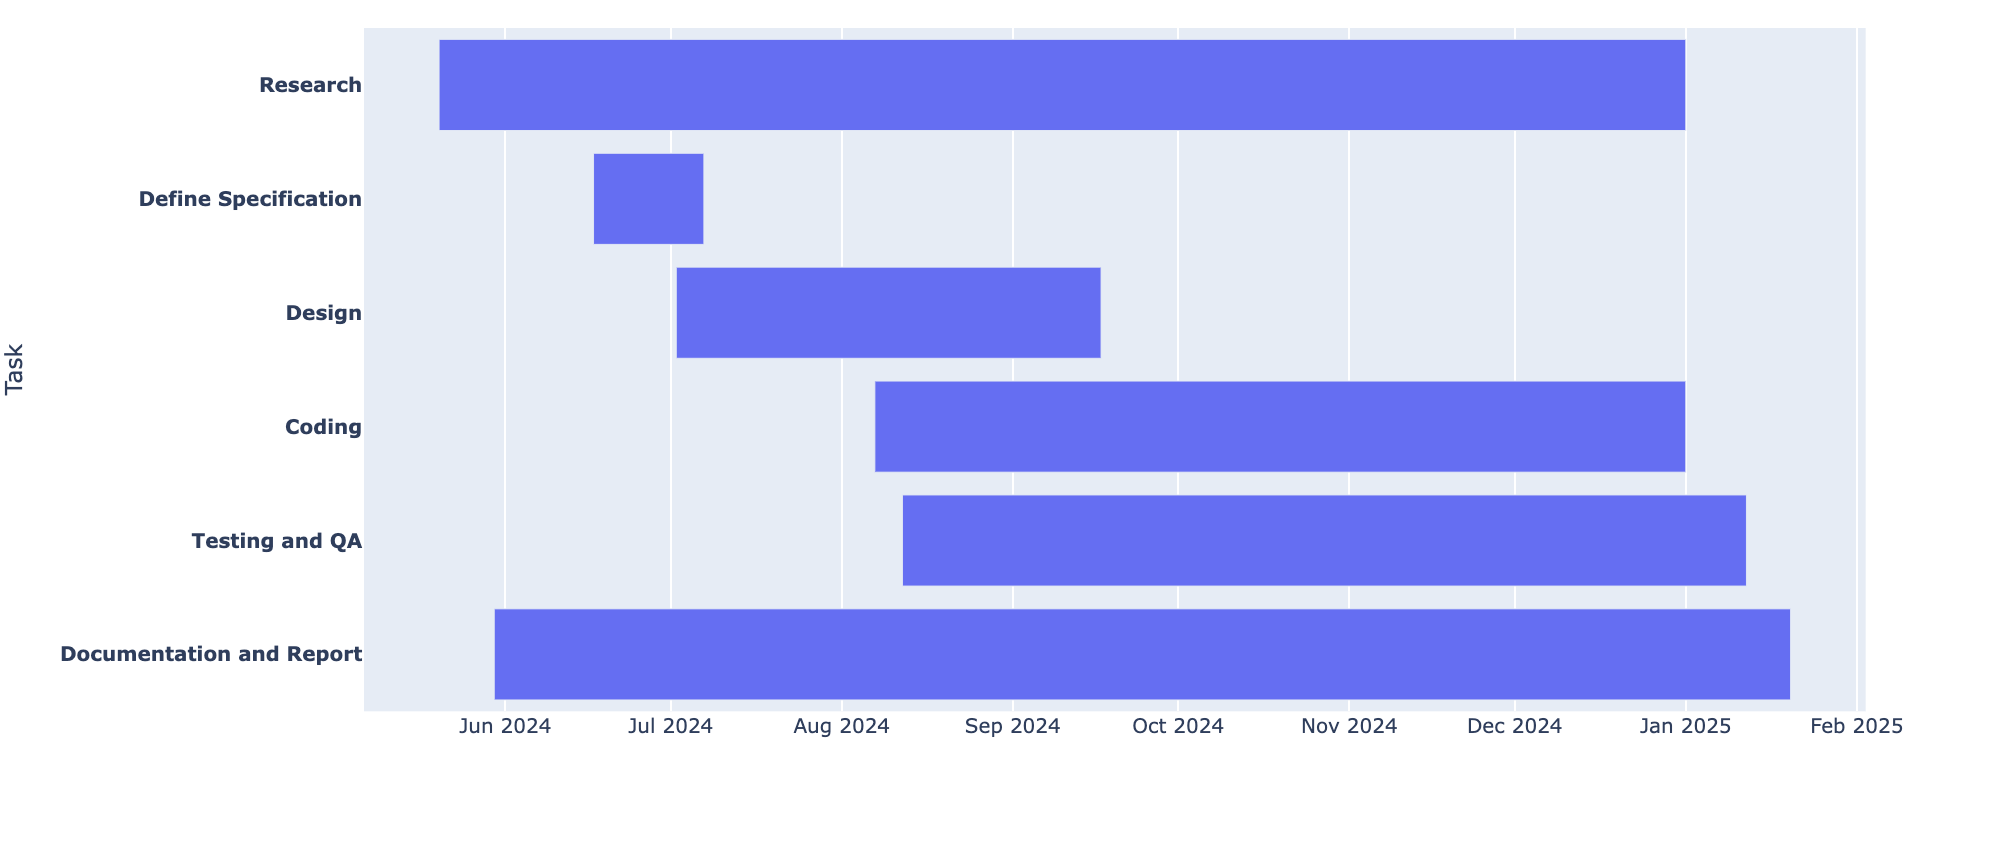
\includegraphics[scale=0.4]{images/GanttChart.png}
    \caption{Gantt Chart}\label{fig:my_label}
\end{figure}
\newpage
\section{System Requirements}

\subsection{Development Requirements}
\begin{table}[h]
    \centering
    \caption{Development Requirements}
    \begin{tabular}{|l|l|}
        \hline
        \textbf{Software Requirements}                 & \textbf{Hardware
        Requirements}                                                          \\ \hline
        Programming Language: Python, Dart, Javascript & RAM: \(>\)= 8 GB
        Megapixels                                                             \\ \hline
        Design Tools: Figma, Canva, Draw.io            & CPU: i5 10th
        \\ \hline
        Libraries: Librosa, PyAudio, Pytorch           & GPU: P100
        (Recommended)                                                          \\ \hline
        Framework: Flutter, Django RestFramework       & Storage: \(>\)= 50 GB
        \\ \hline
        IDEs: VSCode, Android Studio                   &
        \\ \hline
    \end{tabular}
\end{table}

\subsection{Deployment Requirements}
\begin{table}[ht]
    \centering
    \caption{Deployment Requirements}
    \begin{tabular}{|l|l|}
        \hline
        \textbf{Software Requirements} & \textbf{Hardware Requirements}
        \\ \hline
        Android: \(>\)= 10             & RAM: \(>\) 4 GB
        \\ \hline
        Read/Write FileSystem          & Storage: \(>\)= 20 GB
        \\ \hline
        Internet Accessibility         & Recording Quality \(>\)= 256 Kbps, 48
        KHz
        \\ \hline
        Database: MySQL             &                                       \\ \hline
    \end{tabular}
\end{table}

\chapter{Literature Review}

This literature review explores the progression of methodologies and
technologies in the field, with a particular focus on the use of Convolutional
Neural Networks (CNN) and Long Short-Term Memory (LSTM) networks for
audio-based bird species identification. The review also examines the
challenges associated with dataset quality and diversity, and the innovative
strategies employed to address these issues, providing a comprehensive overview
of the current state of research and future directions in avian bioacoustics.

\section{Related Works}
BirdNET is a cutting-edge research platform developed through collaboration
between the K. Lisa Yang Center for Conservation Bioacoustics at the Cornell
Lab of Ornithology and the Chair of Media Informatics at Chemnitz University of
Technology. Its primary aim is to detect and classify bird sounds using machine
learning technologies, serving both experts and citizen scientists in their
efforts to monitor and protect bird populations.\\\\ BirdNET can identify
around 3,000 of the world's most common bird species, with plans to expand this
number. Features such as a live submissions map and a Twitter bot are included
to engage the community and share real-time data. The project is supported by
donations and collaborations, offering opportunities for researchers and
developers to contribute to its growth. BirdNET serves as an invaluable tool
for bird enthusiasts, conservationists, and biologists alike, providing
innovative solutions for large-scale acoustic monitoring and contributing to
the conservation and understanding of avian biodiversity.\\\\ The BirdCLEF 2023
competition on Kaggle is a significant data science challenge that falls under
the broader LifeCLEF initiative, aimed at pushing the boundaries of species
identification and biodiversity monitoring through technological innovation.
This particular competition focuses on the development of machine learning
models that can identify bird species based on audio recordings. It presents a
complex and realistic challenge due to the diversity of the audio recordings,
which are collected from various environments and feature a wide range of bird
species.
\section{Related Research}

The study\cite{gautam2023audio} "Audio Classifier for Automatic Identification
of Endangered Bird Species of Nepal" focuses on using deep learning techniques
to identify endangered bird species from audio recordings. The dataset,
collected from xeno-canto.org, comprises 2215 audio recordings of 41 bird
species, 38 of which are endangered. This dataset was expanded to 6733
recordings through 10-second audio splitting and Gaussian noise augmentation,
with 5407 recordings used for training, 639 for validation, and 687 for
testing. The methodology involved handling imbalanced class distribution
through data augmentation, employing Mel spectrograms and Mel-Frequency
Cepstral Coefficients (MFCCs) for feature extraction, and developing a custom
Convolutional Neural Network (CNN) model and an EfficientNet model. The
hyperparameters of these models were optimized using a genetic algorithm. The
Mel spectrograms were created using Short-Time Fourier Transform, converting
amplitudes to decibel scale, and applying Mel filter banks to the spectrograms.
Similarly, MFCCs were derived by framing the audio signals, applying Discrete
Fourier Transform, logarithmic scaling, Mel scaling, and Discrete Cosine
Transform. The EfficientNet architecture utilized compound scaling for network
depth, width, and resolution. The findings indicated that the proposed approach
achieved satisfactory results in classifying the bird species. Model I, using
Mel Spectrogram and EfficientNet, achieved an F1-score of 79\%, while Model II,
using Mel Spectrogram and Custom CNN, achieved 64\%, and Model III, using MFCC
and EfficientNet, achieved 72\%. However, limitations include the relatively
small dataset size and the need for further enhancement in model robustness and
accuracy.
%Future enhancements could involve
% expanding the dataset, exploring additional feature extraction techniques, and
% incorporating more advanced deep learning models to improve classification
% performance.\cite{gautam2023audio}\\

Sevilla et al.\cite{sevilla2017audio} introduced an innovative approach to bird
sound classification with their study `Audio Bird Classification with
Inception-v4 extended with Time and Time-Frequency Attention Mechanisms'. The
datasets employed include various bird sounds, prominently from the
BirdClef2017 challenge, consisting of 1500 bird species recordings. The
methodology revolves around treating bird sound classification as an image
classification problem through transfer learning. The Inception-v4 model,
initially pre-trained on ImageNet, was adapted to process time-frequency
representations of bird sounds by converting these sounds into RGB images using
three log-spectrograms generated via fast Fourier transform at different scales
(128, 512, 2048 bins).The findings demonstrate that the model, termed
`Soundception', integrates time and time-frequency attention mechanisms
effectively, significantly improving classification accuracy. The results
highlight Soundception's outstanding performance, achieving a mean average
precision (MAP) of 0.714 in classifying 1500 bird species, 0.616 MAP for
background species, and 0.288 MAP for soundscapes with time-codes, making it
the top model in the BirdClef2017 challenge across multiple tasks. However,
limitations include the incomplete convergence of the model due to
computational constraints and the extensive GPU resources required for
training. The paper concludes with a discussion on future improvements, such as
exploring different scalable optimizations and incorporating stacked GRU layers
for better audio-to-image representation learning, underscoring the potential
of transfer learning from advanced image classification models to acoustic
domains.\\

The study, conducted by Chandu B et al.\cite{chandu2020automated}, outlines a
robust methodology for identifying bird species from audio recordings,
leveraging a combination of meticulously curated datasets and machine learning
techniques. The dataset was manually compiledThe working mechanism for bird
identification from audio utilizes the dataset compiled from Xeno Canto,
housing a diverse collection of avian vocalizations. Our methodology revolves
around the utilization of EfficientNet, a state-of-the-art convolutional neural
network architecture known for its balance between accuracy and efficiency.

The primary objective of this study is to achieve high levels of accuracy in
identifying a broad spectrum of 41 distinct bird species. Here lies the
detailed explanation of the methodology, from the working mechanism to model
training. from both local recordings and online resources such as
xeno-canto.org, which apart from bird songs also contains ambient noise and
human voices to simulate real-world conditions. Pre-processing techniques
including pre-emphasis, framing, silence removal, and reconstruction were
applied to the audio clips to enhance the relevant frequency components and
eliminate unnecessary noise, ensuring the purity of the dataset. Spectrograms
of these processed clips were generated and used as input for training a
convolutional neural network (CNN), specifically AlexNet, chosen for its high
accuracy in image classification tasks. Through transfer learning, AlexNet was
adapted to recognize bird species from the spectrograms, achieving a
classification accuracy of 97\% in controlled environments. However,
recognizing the variability of real-world conditions, the researchers retrained
the model with datasets containing ambient noise, achieving a real-time
classification accuracy of 91\%. Despite these promising results, the study
acknowledges limitations such as the relatively small size of the dataset and
the need for further tuning of performance parameters to improve robustness.\\

In\cite{nanni2021ensemble} `An Ensemble of Convolutional Neural Networks for
Audio Classification' delves into a comprehensive study on CNN classification
using different architectures, data augmentation techniques, and audio signal
representations, aimed at enhancing audio classification tasks across various
datasets. The study employs three datasets: BIRDZ, CAT, and ESC-50, each
offering unique challenges in audio classification. The methodology involves
training five convolutional neural networks (CNNs) with four audio
representations combined with six different data augmentation methods,
resulting in thirty-five subtypes of ensembles. The audio representations
include techniques such as the Discrete Gabor Transform (DGT), Waveform
Similarity OverLap Add (WSOLA), and Phase Vocoder. The data augmentation
methods encompass procedures like short spectrogram augmentation, random time
shift, and frequency masking. The CNN architectures are pre-trained models
fine-tuned with these augmented datasets to boost classification accuracy. The
findings reveal that the ensemble method outperforms standalone networks,
achieving 97\% accuracy on the BIRDZ dataset, 90.51\% on the CAT dataset,
andThe working mechanism for bird identification from audio utilizes the
dataset compiled from Xeno Canto, housing a diverse collection of avian
vocalizations. Our methodology revolves around the utilization of EfficientNet,
a state-of-the-art convolutional neural network architecture known for its
balance between accuracy and efficiency.

The primary objective of this study is to achieve high levels of accuracy in
identifying a broad spectrum of 41 distinct bird species. Here lies the
detailed explanation of the methodology, from the working mechanism to model
training. 88.65\% on the ESC-50 dataset. The study also highlights that the
best-performing CNNs are VGG16 and VGG19, with DGT as the most effective signal
representation. However, the study acknowledges limitations, such as the
computational cost of training ensembles and the variability in performance
across different augmentation techniques.\\

In\cite{wang2022efficient} `Analysis of bird call datasets sourced from
Xeno-Canto', comprising 72,172 samples from 264 bird species in 16-bit wav
format with a 16 kHz sampling rate. The methodology involved preprocessing the
audio data to filter out low-frequency noise and normalize signal amplitude,
followed by generating Mel Spectrograms and Mel-Frequency Cepstral Coefficients
(MFCCs) as inputs for deep learning models. The Mel Spectrograms were produced
using discrete Fourier transform (DFT), and the MFCCs were derived by applying
discrete cosine transform (DCT) to the Mel Spectrogram. The study employed
various metrics to evaluate the performance of these methods, including ROC
analysis to visualize model effectiveness. Findings indicated that the proposed
models showed significant promise in identifying bird species from their calls,
with improvements in classification accuracy compared to previous approaches.
However, limitations were noted, including potential biases in the dataset due
to uneven sample distribution across species and the challenge of background
noise affecting signal quality. Future work suggested enhancing noise reduction
techniques and exploring more sophisticated neural network architectures to
further improve model robustness and accuracy.\\

The study\cite{pahuja2021sound} by Pahuja et al. conducted an in-depth analysis
of bird species recognition through acoustic monitoring, utilizing a robust
dataset of bird sound samples, meticulously annotated and validated for
accuracy. The dataset, referred to as SD, comprises multispecies bird sound
recordings, each labeled with species name and sample ID, along with
corresponding metadata, providing a comprehensive foundation for model training
and evaluation. Methodologically, the research employed a spectrogram-based
feature extraction approach, leveraging Short-Time Fourier Transform (STFT) to
capture the intricate temporal and spectral characteristics of bird sounds.
This was followed by the application of a Multilayer Perceptron (MLP)
classifier to distinguish between different bird species. The findings reveal
that the proposed model achieved high recognition accuracy, with some species
being identified with perfect precision, recall, and accuracy (100\%), though
the performance varied across species, with a few showing lower recognition
rates (86.9\%) and precision/recall values ranging between 50\-75\%. The
results demonstrated an overall classification accuracy of 96\%, with
cross-validation accuracy standing at 81.4\%, highlighting the model's
robustness yet indicating room for improvement in generalizability across
diverse datasets. Despite the promising results, the study acknowledges several
limitations, including the variability in recognition accuracy among different
species and the potential influence of environmental noise on model
performance. Future work is suggested to explore feature and model fusion
techniques, integrate the model with cloud-based systems for real-time
recognition, and expand the dataset to include a broader range of bird species
to enhance the model's applicability and accuracy in practical scenarios.\\

The dataset used in this study\cite{carvalho2023automatic} comprises recordings
labeled by species from California and Nevada, USA. It includes 91 species,
with 30 audio samples per species, amounting to a total of 2,730 MP3 files. The
methodology adopted involves three main steps: pre-processing, feature
extraction, and deep learning modeling. For feature extraction, MFCCs were
obtained using the Python library python\_speech\_features, with parameters
such as sample rate, 13 cepstrum coefficients, 26 filterbank filters, and an
FFT size of 512. Mel spectrograms were extracted using the Librosa library,
employing parameters such as a sample rate, an FFT window size of 2048, a hop
length of 512, and 128 Mel bands. In the deep learning modeling, CNNs and LSTMs
were compared for their effectiveness in classifying bird sounds. CNNs
demonstrated superior training accuracy with Mel spectrogram features,
achieving 99.05\% and 98.76\% accuracy for 3-second and 1.5-second spectroThe
working mechanism for bird identification from audio utilizes the dataset
compiled from Xeno Canto, housing a diverse collection of avian vocalizations.
Our methodology revolves around the utilization of EfficientNet, a
state-of-the-art convolutional neural network architecture known for its
balance between accuracy and efficiency.

The primary objective of this study is to achieve high levels of accuracy in
identifying a broad spectrum of 41 distinct bird species. Here lies the
detailed explanation of the methodology, from the working mechanism to model
training.grams, respectively. In contrast, LSTMs achieved lower training
accuracies of 75.85\% and 73.29\% under similar conditions.These results
highlight the superior ability of CNNs to leverage the spatial and
frequency-related patterns in Mel spectrograms for accurate bird species
classification.\\

Finally, in the study\cite{lasseck2018acoustic}, 'Acoustic Bird Detection with
Deep Convolution Neural Network', DCNNs pretrained on ImageNet, have been used
for bioacoustic classification, with preprocessing and augmentation playing
crucial roles in model performance. The preprocessing pipeline typically
involves applying a shallow high-pass filter (Q = 0.707) with a 2 kHz cutoff,
resampling to 22,050 Hz, and extracting around 4-second audio chunks, which are
transformed into mel spectrograms with 310 mel bands (160-10,300 Hz). Further
processing includes removing extreme frequencies, normalizing power
spectrograms to decibel units, resizing to 224*224, and converting grayscale
spectrograms to RGB for compatibility with ResNet. To improve generalization,
data augmentation techniques such as jittering chunk duration, extracting
chunks from random positions, adding noise from unrelated audio files, and
applying random amplitude scaling are employed. Additional augmentations in the
frequency domain include frequency shifting/stretching, piecewise
time/frequency resizing, and color jittering (brightness, contrast, saturation,
hue). Among these, the most effective methods are noise addition from random
files, piecewise time and frequency stretching, and time interval dropout,
which enhance robustness by simulating real-world variations in bird
vocalizations.\\

\newpage

\chapter{Methodology}
This chapter describes the overall system including the bird sound detection
and bird species classification.

% System Architecture
\section{System Overview}
\begin{figure}[h!]
    \centering
    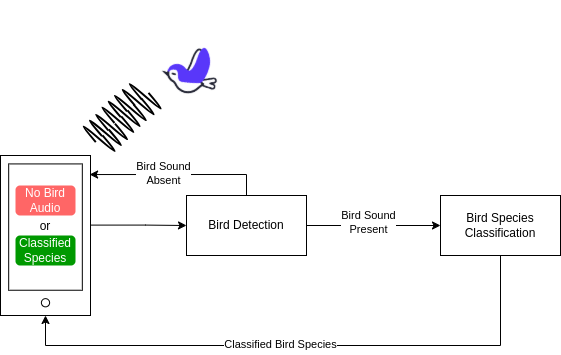
\includegraphics[scale=0.65]{images/System Overview.png}
    \caption{System Overview}\label{fig:system_overview}
\end{figure}
Our project leverages a mobile application to capture audio recordings, which
are then processed to identify bird species. The mobile app records the sound
and visualizes it with waveforms during the recording process. Once the audio
is captured, it is sent to our backend system for further analysis.

This model determines whether
the recorded audio contains bird sounds. If bird sounds are detected, the audio
is then forwarded to the bird species classifier model. The classifier
identifies the specific bird species present in the recording. If the bird sound detection model does not detect any bird
sounds, the recorded audio is labeled accordingly, indicating the absence of
bird sounds.

Upon successful classification, the system maps the identified bird species to
the location where the audio was recorded, utilizing the device's GPS data.
This approach ensures that only relevant audio recordings are processed for
species classification, enhancing the accuracy and efficiency of the system.
The integration of Django, Django Rest Framework, and MySQL provides a robust
and scalable backend infrastructure to support the application's functionality
as shown in Figure \ref{fig:system_overview}.
\\





\section{Working Mechanism for Bird Sound Detection}
      % description about mechanism
      % Image of the Working Mechanism
      \begin{figure}[h!]
            \centering
            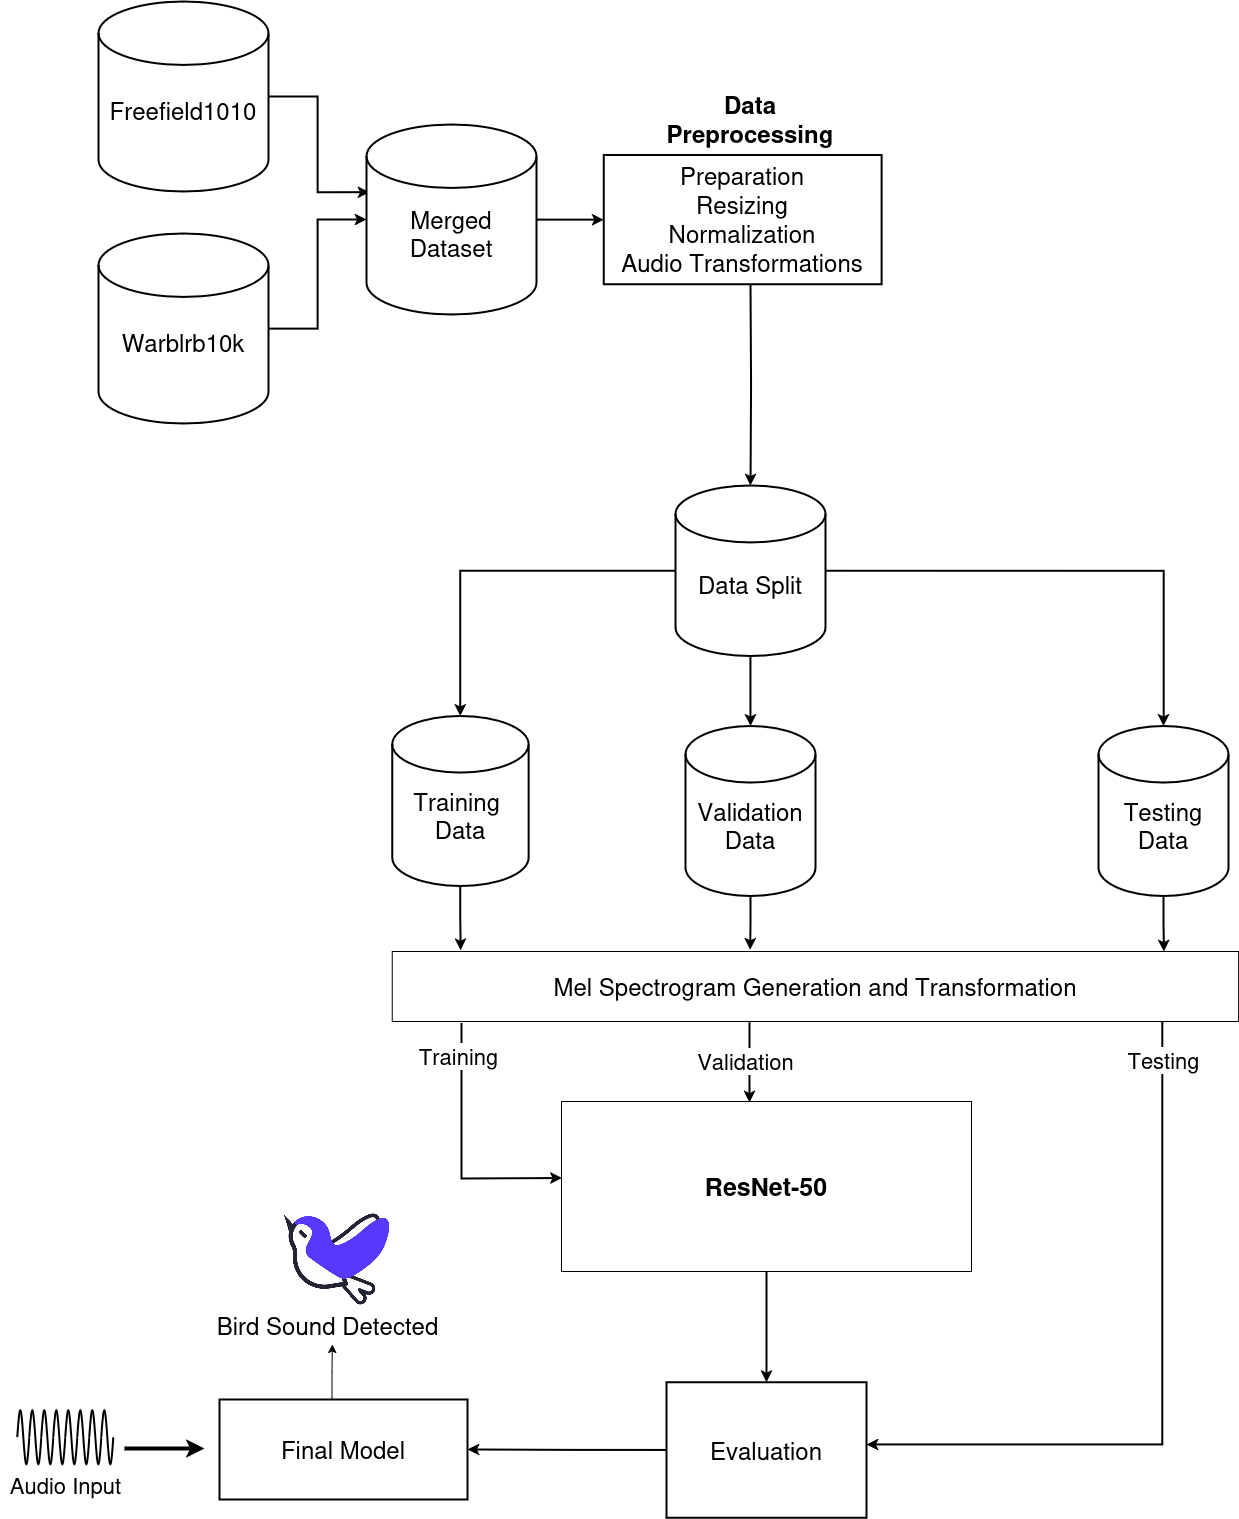
\includegraphics[scale=0.33]{images/MajorProject-Detection.png}
            \caption{Block diagram for the working mechanism for Bird Detection}%\label{fig:fig1}
      \end{figure}

      \subsection{Data Collection}
      The dataset used for the Bird Sound Detection Model includes Field recordings, worldwide ("freefield1010") - a collection of 7,690 excerpts from field recordings around the world, gathered by the FreeSound project, and then standardised for research. This collection is very diverse in location and environment, and for the BAD Challenge, it has been annotated for the presence/absence of birds.
      \begin{figure}[h!]
            \centering
            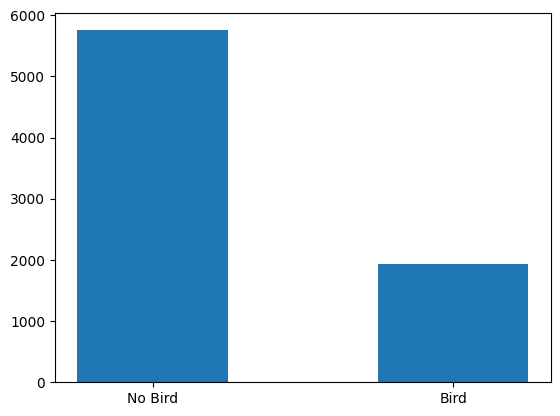
\includegraphics[scale=0.75]{images/dataset_detection-1.png}
            \caption{Dataset distribution for freefield1010}
            \label{fig:freefield1010 dataset}
      \end{figure}
      
      Another dataset used is the Crowdsourced dataset, UK ("warblrb10k") - 8,000 smartphone audio recordings from around the UK, crowdsourced by users of Warblr, the bird recognition app. The audio covers a wide distribution of UK locations and environments and includes weather noise, traffic noise, human speech, and even human bird imitations.
      \begin{figure}[h!]
            \centering
            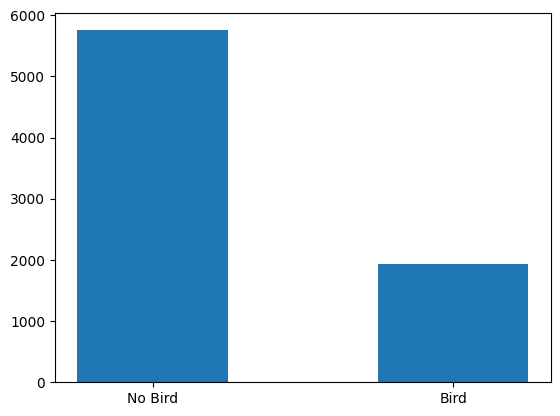
\includegraphics[scale=0.75]{images/dataset_detection-2.png}
            \caption{Dataset distribution for warblrb10k}
            \label{fig:warblrb10k dataset}
      \end{figure}
      \newpage
      Instead of using the datasets separately, we merged them to create a single dataset comprising 15,690 audio recordings—7,710 without bird sounds and 7,980 with bird sounds. The merged dataset was then partitioned into training, testing, and validation sets in an 80:10:10 ratio, ensuring a comprehensive and balanced dataset for model training and evaluation.
      \begin{figure}[h!]
            \centering
            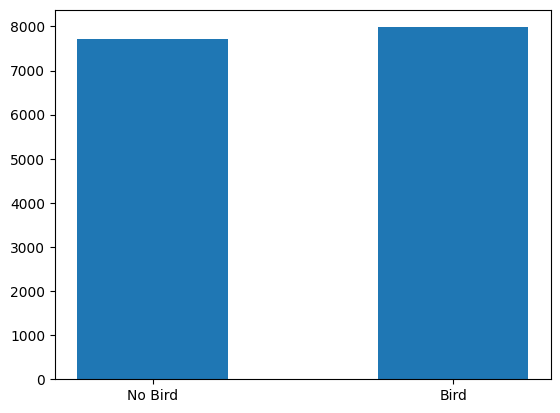
\includegraphics[scale=0.75]{images/dataset_detection-3.png}
            \caption{Distribution of the merged dataset}
            \label{fig:merged_dataset}
      \end{figure}         \newpage      

      \subsection{Data Transformation}
      To enhance the robustness and generalization of our bird sound detection model, we applied a series of transformations on both the raw audio signals and their corresponding Mel Spectrograms. These transformations include:

      \begin{itemize}
            \item \textbf{Add Gaussian Noise (Raw Audio):}\\
            This transformation adds Gaussian noise to the raw audio signal. The noise is generated with a specified mean and standard deviation, and it is added to the audio signal with a certain probability. This helps in making the model robust to noisy environments.
            \begin{equation}
            \text{noise} = \mathcal{N}(\mu, \sigma^2)
            \end{equation}

            \item \textbf{Random Volume Scaling (Raw Audio):}\\
            This transformation scales the volume of the raw audio signal by a random factor within a specified range. The scaling is applied with a certain probability, making the model resilient to variations in recording levels.
            \begin{equation}
            \text{audio} = \text{audio} \times \text{gain}
            \end{equation}
            
            \item \textbf{Time Stretch (Raw Audio):}\\
            This transformation stretches or compresses the time axis of the raw audio signal by a random factor within a specified range. The transformed audio is then converted into a Mel Spectrogram, which helps the model to handle variations in speed.
            \begin{equation}
            \text{audio} = \text{TimeStretch}(\text{audio}, \text{rate})
            \end{equation}
            
            \item \textbf{Frequency Masking (Mel Spectrogram):}\\
            This transformation masks a portion of the frequency bins in the Mel Spectrogram. The maximum number of frequency bins to be masked is specified, and the masking is applied with a certain probability. It encourages the model to focus on different frequency components.
            \begin{equation}
            \text{mel\_spec}[f:f+\text{max\_mask}] = 0
            \end{equation}

            \item \textbf{Time Masking (Mel Spectrogram):}\\
            This transformation masks a portion of the time frames in the Mel Spectrogram. The maximum number of time frames to be masked is specified, and the masking is applied with a certain probability. This helps the model to focus on various temporal features.
            \begin{equation}
            \text{mel\_spec}[:, t:t+\text{max\_mask}] = 0
            \end{equation}

            \item \textbf{Random Content Mixing (Mel Spectrogram):}\\
            This transformation mixes the Mel Spectrogram with another randomly selected noise Mel Spectrogram. The mixing ratio is chosen randomly within a specified range, and the mixing is applied with a certain probability. This aids in making the model robust to background noises.
            \begin{equation}
            \text{mel\_spec} = (1 - \text{mix\_ratio}) \times \text{mel\_spec} + \text{mix\_ratio} \times \text{noise\_spec}
            \end{equation}

            \item \textbf{Time Interval Dropout (Mel Spectrogram):}\\
            This transformation randomly drops intervals of time frames in the Mel Spectrogram. The number of intervals and the width of each interval are chosen randomly within specified ranges, applied with a certain probability. This helps the model to cope with missing or corrupted audio segments.
            \begin{equation}
            \text{mel\_spec}[:, t:t+\text{width}] = 0
            \end{equation}
      \end{itemize}

      \subsection{Feature Extraction}
      The Mel Spectrogram transforms raw audio signals into a time-frequency image that captures the essential spectral characteristics required for bird sound detection. As demonstrated by Lasseck et al.\cite{lasseck2018acoustic}, this approach efficiently distinguishes recordings containing bird vocalizations from those without. For a comprehensive explanation of the computation, please refer to the \nameref{sec:feature_extraction}.

      \subsection{Model Architecture}

      The bird sound detection model utilizes a pre-trained ResNet-50 architecture as a feature extractor, which has been modified to process mel spectrogram representations of audio signals. This section provides a detailed explanation of the ResNet-50 architecture and the modifications applied to adapt it for bird sound detection.

      \subsubsection{ResNet-50: A Detailed Overview}
      ResNet-50, or Residual Network-50, is a deep convolutional neural network (CNN) designed to overcome the vanishing gradient problem that commonly arises in deep networks. It achieves this through the use of residual learning, where shortcut connections (skip connections) allow gradients to bypass certain layers, ensuring efficient training even in very deep architectures.

      \subsubsection{Architecture of ResNet-50}
      ResNet-50 consists of multiple convolutional layers arranged into residual blocks. These blocks introduce identity mappings that help the model learn transformations efficiently. The network follows a hierarchical structure where initial layers focus on low-level features such as edges and textures, while deeper layers extract high-level representations.

      The architecture is composed of four main stages, each containing bottleneck residual blocks. Each block consists of three convolutional layers: a \(1\times1\) convolution for dimensionality reduction, a \(3\times3\) convolution for feature extraction, and another \(1\times1\) convolution to restore dimensionality. By utilizing these bottleneck layers, ResNet-50 maintains computational efficiency while preserving representational power.

      Another key component of ResNet-50 is batch normalization, which standardizes feature maps at each layer, leading to stable gradient flow and faster convergence. Additionally, ReLU activation functions introduce non-linearity, allowing the network to learn complex patterns in the data.

      \begin{figure}[h!]
      \centering
      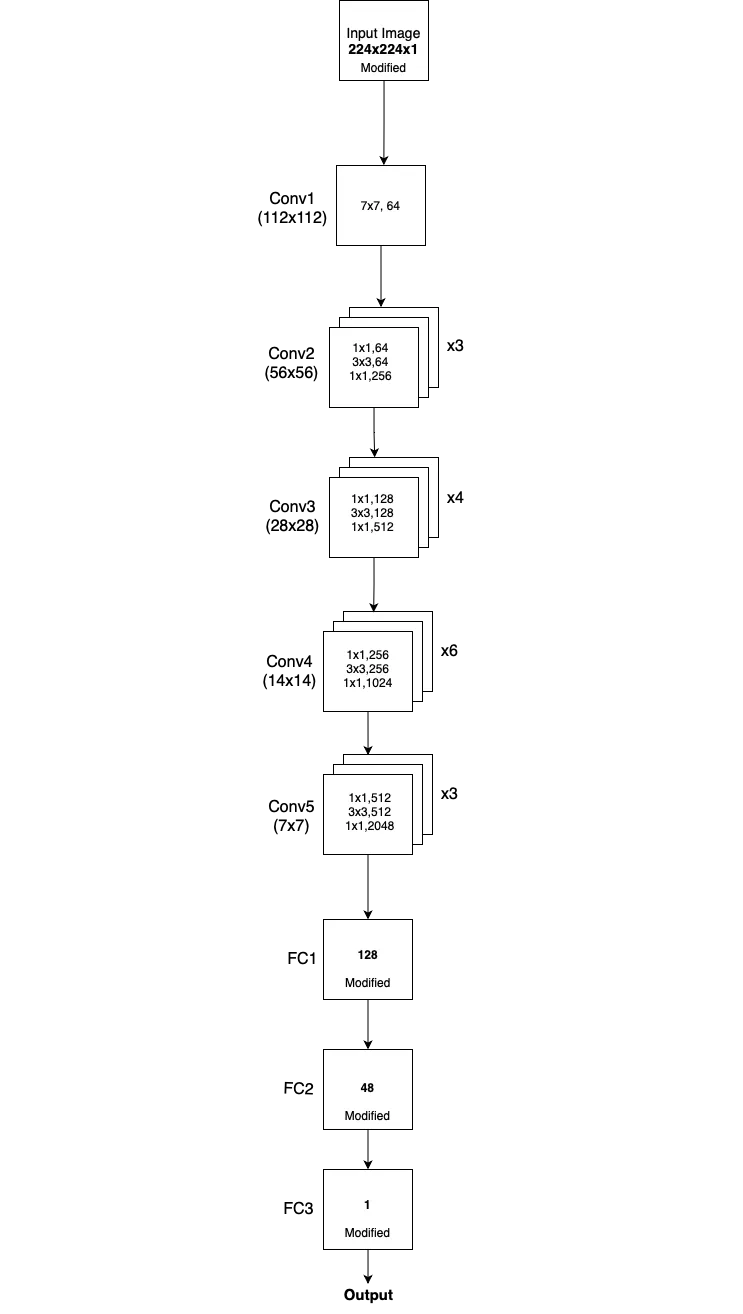
\includegraphics[angle=270,width=0.2\textwidth]{images/MajorProject-resnet architecture.png}
      \caption{Modified ResNet-50 architecture for Bird Sound Detection.}
      \label{fig:resnet50}
      \end{figure}
      \newpage

      \subsubsection{Components of ResNet-50 Architecture}
      The ResNet-50 model consists of several essential components that contribute to its powerful feature extraction and classification capabilities:

      \begin{itemize}
            \item \textbf{Convolutional Layers:} These layers apply convolution operations to extract spatial features from input images. Early layers capture basic features (edges, textures), while deeper layers learn more abstract patterns.
      
            \item \textbf{Batch Normalization:} This technique normalizes activations at each layer to stabilize training, improve convergence, and prevent internal covariate shifts.
      
            \item \textbf{ReLU Activation:} A non-linear activation function that introduces sparsity and helps the network learn complex representations.
      
            \item \textbf{Residual Blocks:} The defining characteristic of ResNet, these blocks contain skip connections that allow gradients to bypass certain layers, mitigating the vanishing gradient problem.
      
            \item \textbf{Bottleneck Layers:} Each residual block consists of three convolutional layers: a \(1\times1\) convolution to reduce dimensionality, a \(3\times3\) convolution to extract features, and another \(1\times1\) convolution to restore the original depth.
      
            \item \textbf{Global Average Pooling:} Reduces the dimensionality of feature maps before passing them to the final classification layer, making the network more efficient.
      
            \item \textbf{Fully Connected Layer:} The final layer of the network that performs classification based on extracted features.
      
            \item \textbf{Softmax/Sigmoid Activation:} Applies a probability distribution to the output for classification, with softmax used for multi-class classification and sigmoid used for binary classification.
      \end{itemize}

      \subsubsection{Adaptation for Bird Sound Detection}
      While ResNet-50 is originally designed for image classification, it can be adapted for processing spectrograms, which are visual representations of sound frequencies over time. In this model, several modifications have been applied to tailor ResNet-50 for the bird sound detection task (see Figure~\ref{fig:resnet50}):

      \begin{itemize}
            \item \textbf{Input Modification:} Since spectrograms are typically represented as grayscale images with a single channel, the original ResNet-50 architecture, which expects three-channel RGB images, has been adjusted to accept single-channel inputs. This allows the network to effectively process spectrogram data without requiring redundant channels.
      
            \item \textbf{Feature Extraction:} The pre-trained ResNet-50 model, trained on large-scale image datasets, is used as a feature extractor. The earlier layers remain unchanged, as they capture fundamental patterns useful for various classification tasks. These convolutional layers are frozen, meaning their weights are not updated during training. This strategy ensures that the model benefits from pre-learned visual features while focusing its learning on the final classification task.
      
            \item \textbf{Modified Classification Layer:} The original fully connected classification layer of ResNet-50 has been replaced with a custom classification head optimized for binary classification (presence or absence of bird sound). This new layer stack introduces additional non-linearity and dropout mechanisms to prevent overfitting, ultimately improving the model’s ability to generalize to new data.
      
      \end{itemize}

      \subsubsection{Training and Generalization}
      By freezing the early convolutional layers and training only the newly added classification layers, the model efficiently learns to distinguish bird sounds from other environmental noises. This transfer learning approach significantly reduces the training time and the amount of labeled data required, making the model robust in real-world scenarios.

      The final model is designed to process mel spectrogram inputs and produce a probability score indicating the presence of bird sounds. The use of residual learning allows for deep feature extraction, making the model highly effective in distinguishing between subtle variations in audio patterns.
      
      

      \subsection{Training Process}
      The training process for the bird sound detection model was carefully designed to ensure optimal learning and generalization. The process incorporated several key components and strategies:
      \begin{itemize}
            \item \textbf{Training Parameters:}
            \begin{itemize}
                  \item Number of epochs: 20
                  \item Batch size: 32
                  \item Initial learning rate: 0.001
                  \item Weight decay: 0.0001
            \end{itemize}

            \item \textbf{Loss Function:}
            Binary Cross-Entropy Loss (BCE) was chosen as the loss function due to its effectiveness in binary classification tasks. For input predictions $\hat{y}$ and true labels $y$, the BCE loss is calculated as:
            
            % here
            
            % \begin{equation}
            \begin{eqnarray}
                  L_{BCE} = -\frac{1}{N}\sum_{i=1}^{N}[y_i\log(\hat{y}_i) + (1-y_i)\log(1-\hat{y_i})]
            % \end{equation}
            \end{eqnarray}
                  where N is the number of data samples.

            \item \textbf{Optimization:}
            \begin{itemize}
                  \item The Adam optimizer was employed with the following parameters:
                        \begin{itemize}
                              \item Learning rate: 0.001
                              \item Weight decay: 0.0001
                        \end{itemize}
                  \item Learning rate scheduling was implemented using ReduceLROnPlateau with:
                        \begin{itemize}
                              \item Reduction factor: 0.1
                              \item Patience: 3 epochs
                        \end{itemize}
            \end{itemize}

            \item \textbf{Monitoring and Validation:}
            \begin{itemize}
                  \item Training and validation losses were monitored each epoch
                  \item Learning rate adjustments were made based on validation loss plateaus
                  \item Early stopping was implemented to prevent overfitting
                  \item Model performance was evaluated on the test set after training completion
            \end{itemize}
      \end{itemize} 
      The key hyperparameters used for training are summarized in Table \ref{tab:training_hyperparameters}.
      \begin{table}[h]
            \centering
            \caption{Training Hyperparameters}
            \label{tab:training_hyperparameters}
            \begin{tabular}{|c|c|}
                \hline
                \textbf{Hyperparameter} & \textbf{Value} \\
                \hline
                Number of Epochs & 20 \\
                \hline
                Batch Size & 32 \\
                \hline
                Initial Learning Rate & 0.001 \\
                \hline
                Weight Decay & 0.0001 \\
                \hline
                Loss Function & Binary Cross-Entropy (BCE) \\
                \hline
                Optimizer & Adam \\
                \hline
                Learning Rate Scheduling & ReduceLROnPlateau \\
                \hline
                Reduction Factor & 0.1 \\
                \hline
                Patience & 3 epochs \\
                \hline
                Early Stopping & Patience = 3 epochs \\
                \hline
            \end{tabular}
      \end{table}
            
            
      \subsection{Evaluation}
      To assess the effectiveness of our model in distinguishing between the target classes, we analyzed its performance using the Receiver Operating Characteristic (ROC) curve. Following the benchmark established by Lasseck et al.\cite{lasseck2018acoustic} for the freefield1010 and warblrb10k datasets, the Area Under the Curve (AUC) metric was chosen as the primary evaluation criterion.

      The ROC curve provides a comprehensive visualization of the model's discriminative ability by plotting the True Positive Rate (TPR) against the False Positive Rate (FPR) at various classification thresholds. For our binary classification task:

      \begin{itemize}
      \item \textbf{True Positive Rate (Sensitivity):}
      \begin{equation}
            TPR = \frac{TP}{TP + FN}
      \end{equation}
      Measures the proportion of actual bird sounds correctly identified.

      \item \textbf{False Positive Rate (1 - Specificity):}
      \begin{equation}
            FPR = \frac{FP}{FP + TN}
      \end{equation}
      Represents the proportion of non-bird sounds incorrectly classified as bird sounds.
      \end{itemize}
 `    '
      The Area Under the ROC Curve (AUC) provides a single scalar value representing the model's overall classification performance. An AUC of 1.0 represents perfect classification, while 0.5 indicates random chance performance.

      The ROC curve analysis reveals several important aspects of our model's performance:

      \begin{itemize}
      \item \textbf{Threshold Independence:} The ROC curve demonstrates the model's performance across all possible classification thresholds, providing a more robust evaluation than single-threshold metrics.
      
      \item \textbf{Class Imbalance Handling:} Unlike accuracy, the ROC curve remains effective even when dealing with imbalanced datasets, making it particularly suitable for real-world bird sound detection scenarios.
      
      \item \textbf{Operating Point Selection:} The curve enables the selection of optimal decision thresholds based on specific requirements for sensitivity versus specificity in deployment scenarios.
      \end{itemize}

      The high AUC score indicates that our model effectively separates bird sounds from background noise and other environmental sounds, making it reliable for real-world applications in bird sound detection.




\section{Working Mechanism for Bird Species Classification}
        The working mechanism for bird identification from audio utilizes the dataset
        compiled from Xeno Canto, housing a diverse collection of avian vocalizations.
        Our methodology revolves around the utilization of EfficientNet, a
        state-of-the-art convolutional neural network architecture known for its
        balance between accuracy and efficiency.

        The primary objective of this study is to achieve high levels of accuracy in
        identifying a broad spectrum of 41 distinct bird species. Here lies the
        detailed explanation of the methodology, from the working mechanism to model
        training.

        % https://www.geeksforgeeks.org/vgg-16-cnn-model/
        \begin{figure}[h!]
            \centering
            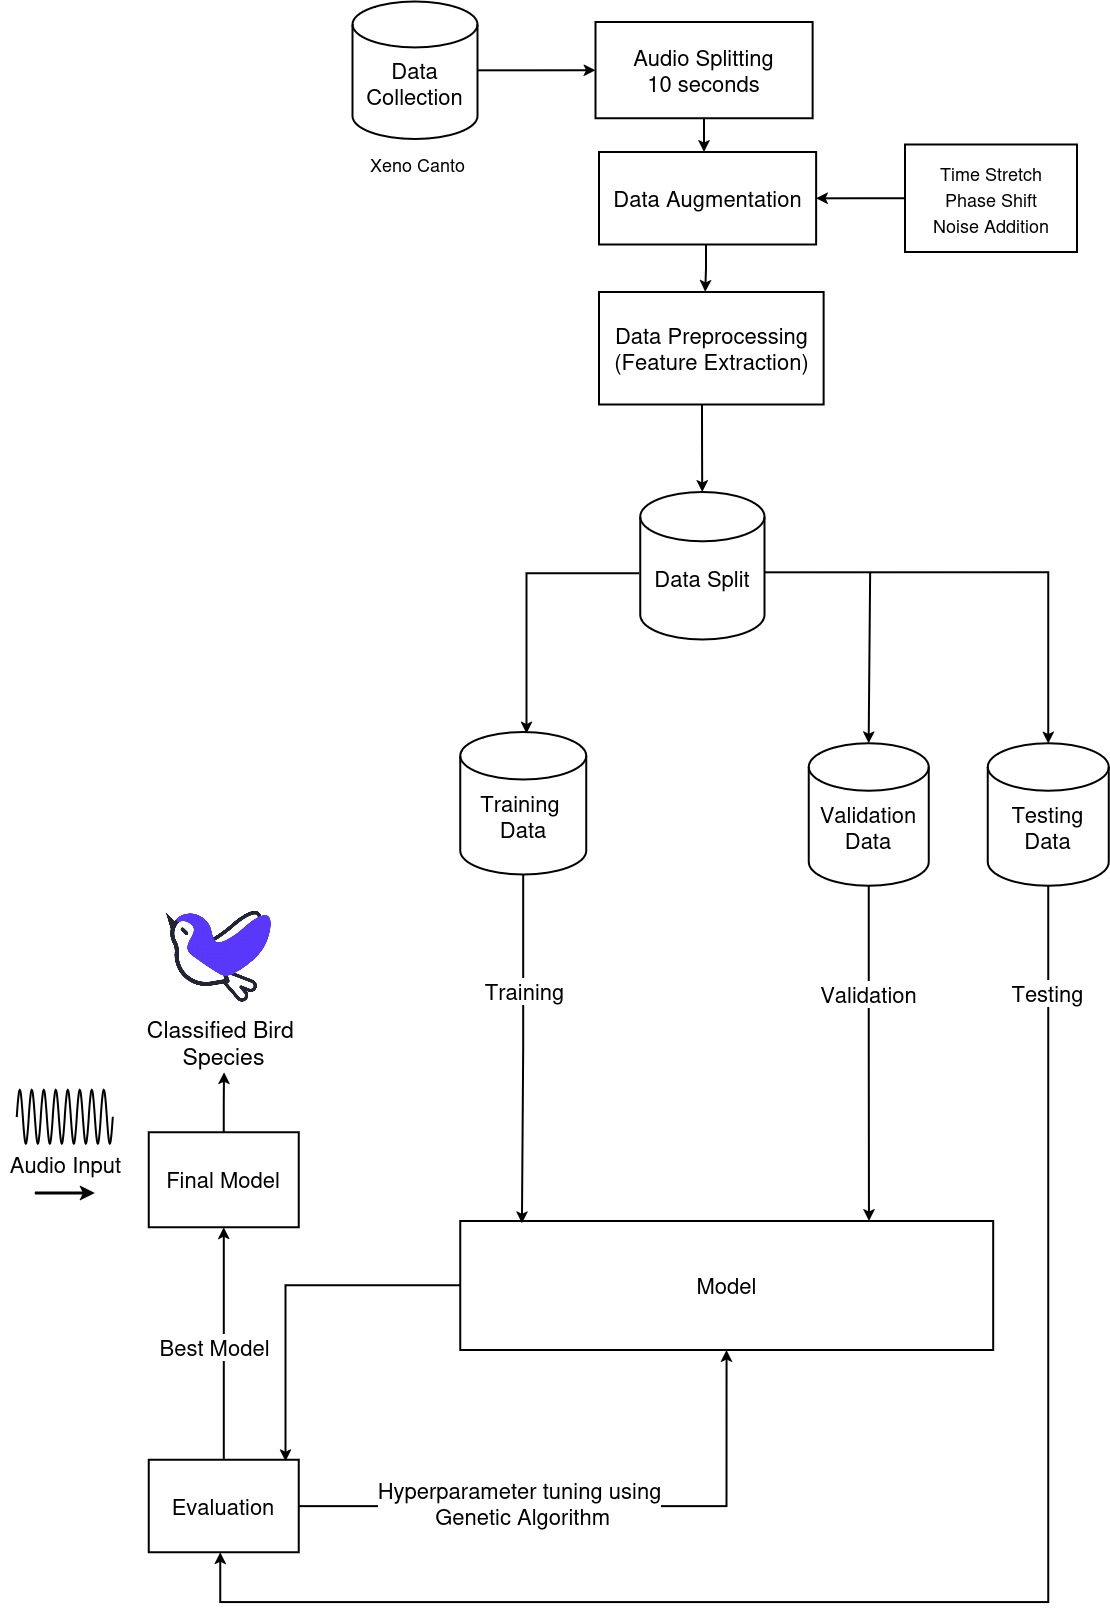
\includegraphics[scale=0.33]{images/MajorProject-Audio Methodology.png}
            \caption{Block diagram for the working mechanism for Bird Species Identification}%\label{fig:fig1}
        \end{figure}


        \subsection{Data Collection}
        For the bird species classification model, we scraped audio data from Xeno-canto
        (\textit{xeno-canto.org}), a global repository of bird vocalizations
        contributed by ornithologists and birding enthusiasts. Since the dataset was
        highly imbalanced, we applied a series of preprocessing and augmentation
        techniques to ensure a more uniform distribution across bird species.
        
        \begin{figure}[h!]
            \centering
            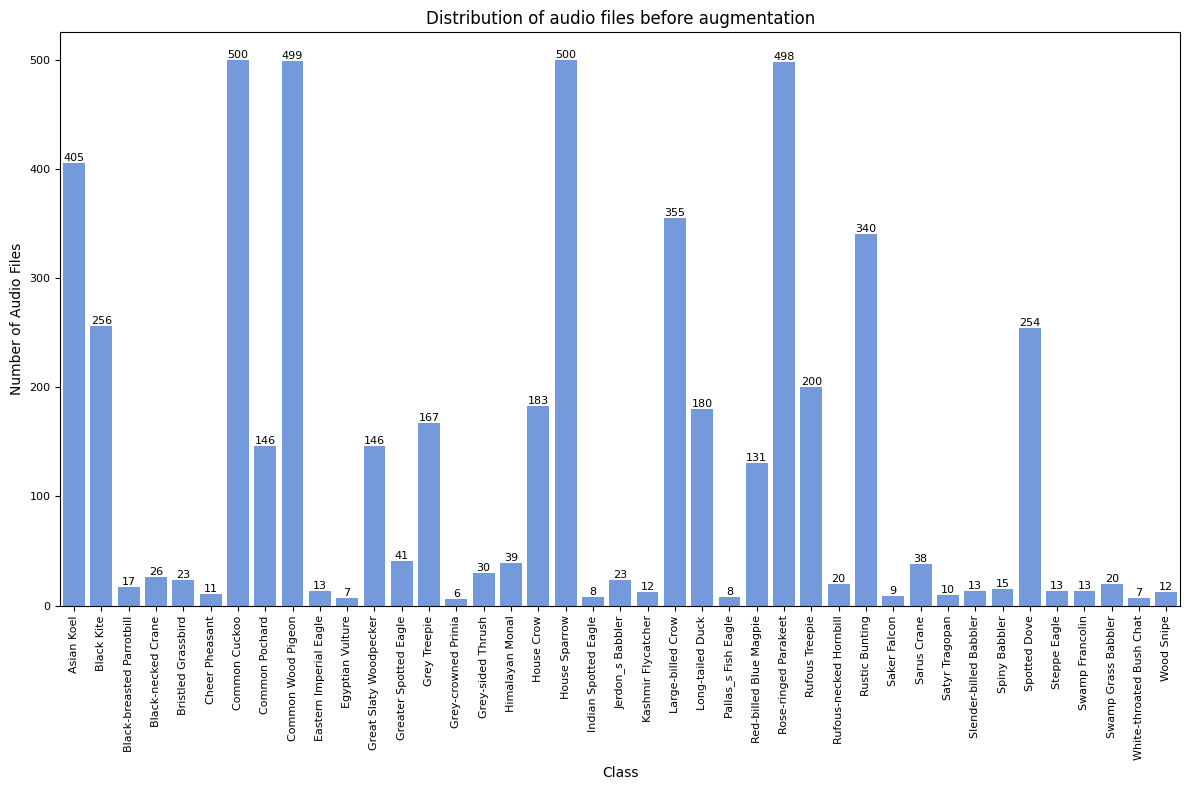
\includegraphics[width=0.8\textwidth]{images/before_augmentation.png}
            \caption{Dataset before performing augmentation}
            \label{fig:visualization}
        \end{figure}

        \subsection{Data Augmentation}
        Initial analysis of the collected data revealed significant class imbalance,
        with some species having over 400 recordings while others had fewer than 50.
        Additionally, the audio recordings varied in length. To address these issues:
        \begin{itemize}
            \item \textbf{Audio Clipping:}
                \begin{itemize}
                    \item Recordings were clipped into segments of 10 seconds each.
                    \item Clips shorter than 5 seconds were discarded to avoid blank audio segments and
                            insufficient data.
                    \item Clips between 5 and 10 seconds were padded with silence at the end to
                            standardize their length to 10 seconds.
                \end{itemize}
        
            \item \textbf{Augmentation Techniques:}
                To balance the dataset, augmentation techniques such as time stretching, phase shifting, and noise addition were applied. The parameters were varied to ensure diversity in the augmented data.
                \begin{itemize}
                    \item Each bird class was augmented to contain exactly 500 audio clips.
                \end{itemize}
        \end{itemize}
        
        \begin{figure}[h!]
            \centering
            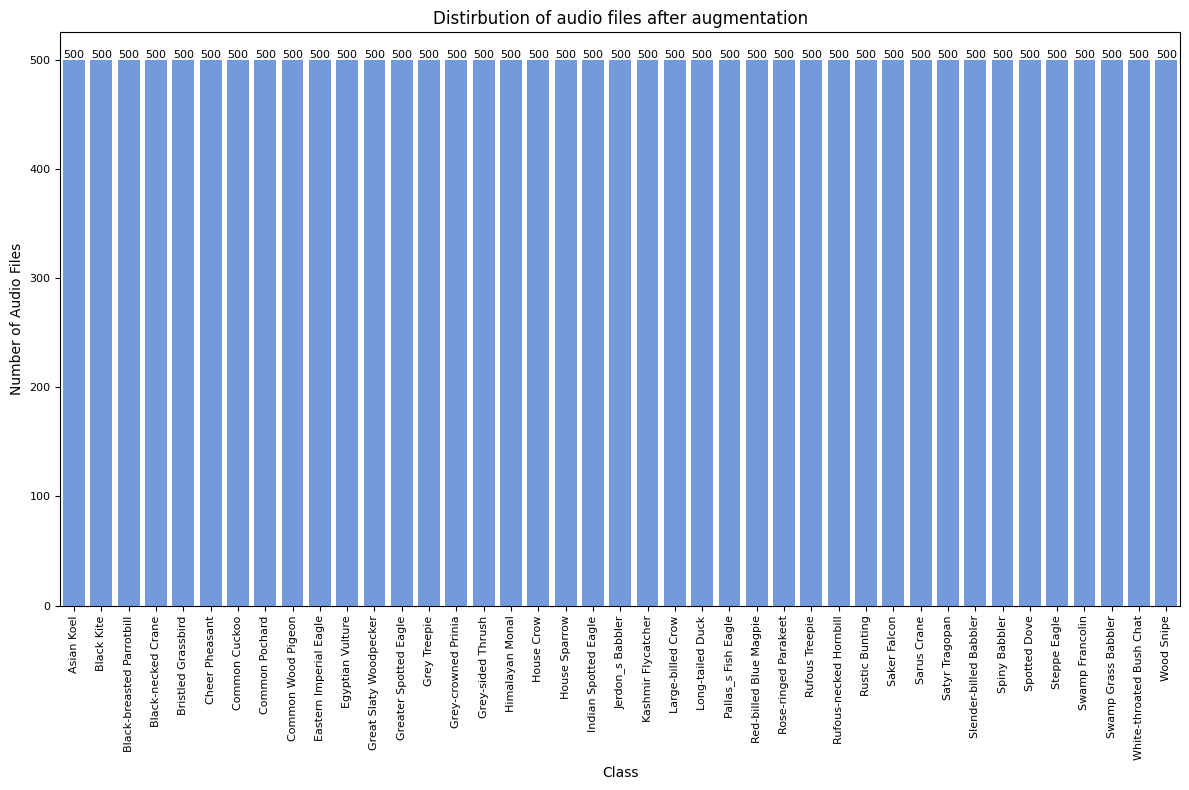
\includegraphics[width=0.8\textwidth]{images/after_augmentation.png}
            \caption{Dataset after performing augmentation}
            \label{fig:visualization}
        \end{figure}

        % Data Preprocessing
        \subsection{Data Preprocessing}
        The audio recordings were transformed into Mel Spectrograms for further
        analysis.

        \begin{itemize}
            \item \textbf{Conversion Details:}
                \begin{itemize}
                    \item Audio files were converted using a sample rate of 32,000 Hz.
                    \item The spectrograms were generated with a Hanning window and 48 Mel bands.
                \end{itemize}

            \item \textbf{Dataset Expansion:}
                \begin{itemize}
                    \item Each audio file was converted into corresponding Mel
                            Spectrogram images for CNN based models and MFCC vectors for LSTM based model.
                    \item The resulting dataset was divided into training, validation, and testing sets
                            for model development.
                \end{itemize}
        \end{itemize} 

      \subsection{Feature Extraction}
      The Mel Spectrogram was employed to transform raw audio recordings into a two-dimensional time-frequency representation, effectively converting sound into an image-like format for processing by convolutional neural networks. This method captures both the temporal and spectral nuances of bird calls, allowing the classifier to discern distinguishing features among various species. As demonstrated in the work of Sevilla et al.\cite{sevilla2017audio}, such time-frequency representations enhance classification accuracy by emphasizing key frequency components inherent in bird vocalizations.

      For a more detailed discussion on the Mel Spectrograms, please refer to the \ref{sec:feature_extraction}.

      
      \subsection{Model Architecture}

      The bird call classification model is based on EfficientNetB3, a deep convolutional neural network (CNN) designed for optimal efficiency and accuracy. EfficientNetB3 achieves this through \textbf{compound scaling}, which uniformly scales network depth, width, and resolution to maximize performance while minimizing computational cost.
      
      \subsubsection{EfficientNetB3}
      EfficientNetB3 is part of the EfficientNet family, which employs a balance between deeper layers, wider networks, and higher input resolutions. This architecture integrates several enhancements, including \textbf{Mobile Inverted Bottleneck Convolution (MBConv) blocks}, \textbf{squeeze-and-excitation (SE) modules}, and the \textbf{Swish activation function}. These components contribute to better feature extraction and gradient flow, ensuring robust classification performance.
      \begin{itemize}
            \item[i] \textbf{Architecture of EfficientNetB3} \\
            EfficientNetB3 follows a hierarchical feature extraction process, where early layers detect fundamental patterns (edges, textures), while deeper layers extract more complex features. The architecture consists of multiple MBConv blocks that improve computational efficiency by using \textbf{depthwise separable convolutions} and \textbf{linear bottlenecks}. Additionally, SE modules dynamically recalibrate channel-wise feature responses, enhancing the model’s ability to focus on important frequency patterns in the mel spectrogram.
            
            \begin{figure}[h!]
                  \centering
                  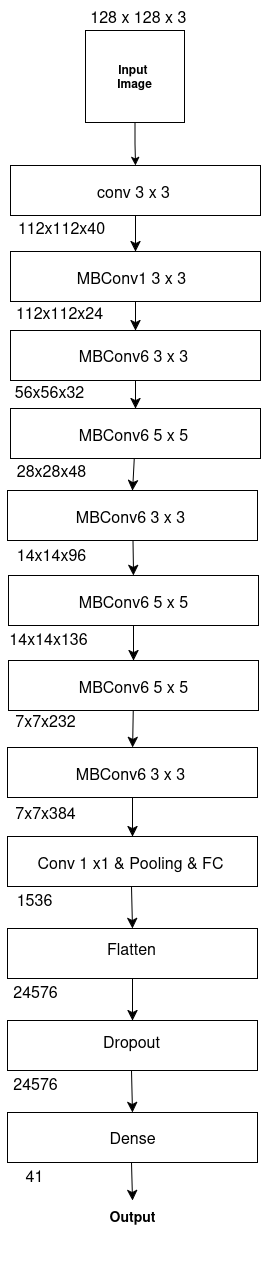
\includegraphics[width=0.3\textwidth]{images/MajorProject-efficientNetB3 architecture.png}
                  \caption{Modified EfficientNetB3 architecture for Bird Species Classification.}
                  \label{fig:efficientnetb3}
            \end{figure}
            
            The key architectural components of EfficientNetB3 are summarized below:
            
            \begin{itemize}
                  \item \textbf{Convolutional Layers:} Extract spatial features from input spectrograms. Early layers capture basic patterns (edges, textures), while deeper layers learn abstract audio representations.
                  
                  \item \textbf{MBConv Blocks:} Mobile Inverted Bottleneck Convolution blocks enhance efficiency by using depthwise separable convolutions and linear bottlenecks.
                  
                  \item \textbf{Squeeze-and-Excitation (SE) Modules:} Improve feature recalibration by dynamically adjusting channel-wise feature responses, allowing the network to focus on relevant frequency patterns.
                  
                  \item \textbf{Swish Activation:} A smooth, non-monotonic activation function that enhances gradient flow and optimization stability.
                  
                  \item \textbf{Batch Normalization:} Standardizes activations at each layer to stabilize training and improve convergence.
                  
                  \item \textbf{Global Average Pooling:} Reduces dimensionality of feature maps before passing them to the classification layer.
                  
                  \item \textbf{Dropout Layer:} A dropout rate of 0.3 is applied to prevent overfitting by randomly deactivating neurons.
                  
                  \item \textbf{Fully Connected Layer:} Converts extracted features into classification outputs.
                  
                  \item \textbf{Softmax Activation:} Generates probability distributions for multi-class classification.
            \end{itemize}
            
            
            % \subsubsection{Adaptation for Bird Call Classification}
            \item[ii)] \textbf{Adaptation for Bird Call Classification} \\
            While EfficientNetB3 is originally designed for image classification, it has been adapted for bird call classification by processing mel spectrograms as input. The key modifications include:
            
            \begin{itemize}
            \item \textbf{Input Modification:} The model accepts spectrogram inputs with dimensions \(128 \times 128 \times 3\), where three channels correspond to different spectrogram augmentations or frequency bands.
            \item \textbf{Feature Extraction:} The EfficientNetB3 layers pre-trained on ImageNet are used as a feature extractor. The convolutional layers are \textbf{frozen} to retain general visual features while training the classification head on bird call data.
            \item \textbf{Custom Classification Head:} The original fully connected layers are replaced with a new classification head consisting of a \textbf{Flatten} layer, \textbf{Dropout} layer (0.3), and a \textbf{Dense} layer. A softmax activation function is applied to generate class probabilities.
            \end{itemize}
            

            \item[iii)] \textbf{Training and Generalization} \\
            The model is trained using a transfer learning approach, where only the classification layers are updated while the pre-trained EfficientNetB3 layers remain frozen. This reduces training time and improves generalization.
            

            % \subsubsection{Training Process}
            \item[iv)] \textbf{Training Process} 
            \begin{itemize}
                  \item \textbf{Initial Training Parameters:}
                  \begin{itemize}
                  \item Number of epochs: 30
                  \item Batch size: 4
                  \item Image size: \(128 \times 128 \times 3\)
                  \item Initial learning rate: 0.0001
                  \end{itemize}
            
                  \item \textbf{Loss Function:}
                  Categorical Cross-Entropy(CCE) was chosen as the loss function since it is well-suited for multi-class classification tasks. The Categorical Cross-Entropy is calculated as:
                  % \begin{equation}
                  \begin{eqnarray}
                        L_{CCE} = -\frac{1}{N} \sum_{i=1}^{N} \sum_{j=1}^{C} y_{i,j} \log(\hat{y}_{i,j})
                  \end{eqnarray}
                        where N is Number of data samples and C is number of Classes.
                  
                  % \end{equation}
      
            
                  \item \textbf{Optimization:}
                  \begin{itemize}
                  \item The Adam optimizer was employed with the following parameters:
                  \begin{itemize}
                        \item Learning rate: 0.0001
                  \end{itemize}
                  \item Learning rate scheduling was implemented using an exponential decay function after the first five epochs.
                  \end{itemize}
            
                  \item \textbf{Regularization:}
                  \begin{itemize}
                  \item Dropout (0.3) was applied to prevent overfitting.
                  \item L2 regularization (\(\lambda = 1e^{-4}\)) was used for additional weight regularization.
                  \end{itemize}
            
                  \item \textbf{Monitoring and Validation:}
                  \begin{itemize}
                  \item Training and validation losses were monitored each epoch.
                  \item Learning rate adjustments were made using an exponential decay function.
                  \item Early stopping was implemented with a patience of three epochs to prevent overfitting.
                  \item Model checkpointing was applied to save the best-performing model based on validation loss.
                  \end{itemize}
            \end{itemize} 
            
            The key hyperparameters used for training are summarized in Table \ref{tab:training_hyperparameters}.
            \begin{table}[h]
                  \centering
                  \caption{Initial Training Hyperparameters}
                  \label{tab:training_hyperparameters}
                  \begin{tabular}{|c|c|}
                  \hline
                  \textbf{Hyperparameter} & \textbf{Value} \\
                  \hline
                  Number of Epochs & 30 \\
                  \hline
                  Batch Size & 4 \\
                  \hline
                  Input Image Size & \(128 \times 128 \times 3\) \\
                  \hline
                  Initial Learning Rate & 0.0001 \\
                  \hline
                  Loss Function & Categorical Cross-Entropy \\
                  \hline
                  Optimizer & Adam \\
                  \hline
                  Learning Rate Scheduling & Exponential Decay (after 5 epochs) \\
                  \hline
                  Dropout Rate & 0.3 \\
                  \hline
                  L2 Regularization & \(1e^{-4}\) \\
                  % \hline
                  Early Stopping & Patience = 3 epochs \\
                  \hline
                  \end{tabular}
            \end{table}
            
            
            The final model efficiently classifies bird calls by leveraging deep feature extraction from EfficientNetB3 while incorporating a custom classification head optimized for spectrogram data. Through transfer learning and regularization techniques, the model generalizes well to new audio samples, achieving high classification accuracy.
      \end{itemize}


      \subsubsection{CNN+LSTM Model}
      The CNN+LSTM architecture is designed for bird call classification using MFCC (Mel-Frequency Cepstral Coefficients) matrices instead of mel spectrogram images. Unlike EfficientNetB3, which processes image representations of audio, this model extracts both spatial and temporal features by combining convolutional layers with recurrent layers.

      \subsubsection{Architecture of CNN+LSTM}
      This model follows a two-stage feature extraction process:

      \begin{itemize}
      \item \textbf{Convolutional Feature Extraction:} Convolutional layers extract local frequency features from MFCC matrices, capturing patterns in short time frames.
      \item \textbf{Temporal Modeling with LSTM:} A Long Short-Term Memory (LSTM) layer processes sequential dependencies in the extracted features, enhancing temporal understanding.
      \end{itemize}

      The key architectural components of the CNN+LSTM model are as follows:

      \begin{itemize}
      \item \textbf{Convolutional Layers:} Three convolutional layers extract spatial features from MFCC input. Each convolutional block includes:
      \begin{itemize}
            \item \textbf{Conv2D:} Filters of sizes $(3 \times 3)$ with ReLU activation.
            \item \textbf{Batch Normalization:} Normalizes activations for stable training.
            \item \textbf{MaxPooling2D:} Reduces feature map dimensions by pooling along the time axis.
      \end{itemize}
      
      \item \textbf{Time-Distributed Flattening:} Flattens convolutional feature maps while preserving temporal dimensions for LSTM processing.
      
      \item \textbf{LSTM Layer:} A 256-unit LSTM layer captures long-range temporal dependencies in bird call sequences.
      
      \item \textbf{Fully Connected Layers:} Two dense layers process the LSTM output:
      \begin{itemize}
            \item A 64-unit dense layer with ReLU activation and dropout (0.3) for regularization.
            \item An output dense layer with softmax activation for classification.
      \end{itemize}
      \end{itemize}

      \subsubsection{Adaptation for Bird Call Classification}
      The CNN+LSTM model is tailored to classify bird calls based on MFCC matrices instead of image-based spectrograms. The key modifications include:

      \begin{itemize}
      \item \textbf{Input Modification:} The model accepts MFCC matrices with dimensions $(13 \times 626 \times 1)$, where 13 represents MFCC coefficients, and 626 represents time frames.
      \item \textbf{Sequential Feature Extraction:} CNN layers extract spatial frequency information, while the LSTM layer captures sequential dependencies in bird calls.
      \item \textbf{Custom Classification Head:} Includes fully connected layers with dropout to reduce overfitting.
      \end{itemize}

      \subsubsection{Training and Generalization}
      The model is trained using a combination of early stopping, learning rate scheduling, and model checkpointing to ensure optimal performance.

      \subsubsection{Training Process}
      \begin{itemize}
      \item \textbf{Initial Training Parameters:}
      \begin{itemize}
            \item Number of epochs: 30
            \item Batch size: 16
            \item Learning rate: 0.0001
            \item Loss function: Categorical Cross-Entropy
      \end{itemize}
      
      \item \textbf{Optimization:}
      \begin{itemize}
            \item Adam optimizer with an initial learning rate of 0.0001.
            \item Learning rate scheduling using an exponential decay function after the first five epochs.
      \end{itemize}
      
      \item \textbf{Regularization:}
      \begin{itemize}
            \item Dropout (0.3) applied to prevent overfitting.
            % \item L2 regularization to improve generalization.
      \end{itemize}
      
      \item \textbf{Monitoring and Validation:}
      \begin{itemize}
            \item Training and validation losses monitored per epoch.
            \item Early stopping with a patience of 3 epochs.
            \item Model checkpointing to save the best-performing model based on validation loss.
      \end{itemize}
      \end{itemize}

      The key hyperparameters used for training are summarized in Table \ref{tab:training_hyperparameters_cnnlstm}.

      \begin{table}[h]
      \centering
      \caption{Initial Training Hyperparameters for CNN+LSTM}
      \label{tab:training_hyperparameters_cnnlstm}
      \begin{tabular}{|c|c|}
            \hline
            \textbf{Hyperparameter} & \textbf{Value} \\
            \hline
            Number of Epochs & 30 \\
            \hline
            Batch Size & 16 \\
            \hline
            Input Shape & (13, 626, 1) \\
            \hline
            Learning Rate & 0.0001 \\
            \hline
            Loss Function & Categorical Cross-Entropy \\
            \hline
            Optimizer & Adam \\
            \hline
            Learning Rate Scheduling & Exponential Decay (after 5 epochs) \\
            \hline
            Dropout Rate & 0.3 \\
            \hline
            Early Stopping & Patience = 3 epochs \\
            \hline
      \end{tabular}
      \end{table}

      The final CNN+LSTM model effectively classifies bird calls by integrating deep convolutional feature extraction with temporal modeling, ensuring high accuracy while leveraging MFCC representations.



      %   \subsection{Training Process}
      %   The training process utilizes the \textbf{categorical cross-entropy loss function}, which is suitable for multi-class classification problems. The Adam optimizer with a learning rate of \textbf{0.0001} was used to update model weights, and the model was trained for \textbf{30 epochs} with callbacks to enhance performance and prevent overfitting.
        
      %   A learning rate scheduler was implemented to adjust the learning rate dynamically. For the first five epochs, the learning rate remains constant, after which it follows an \textbf{exponential decay function}. Additionally, \textbf{early stopping} was employed, monitoring the validation loss with a patience of \textbf{3 epochs}, ensuring that the best model weights are restored. A \textbf{model checkpoint} callback saves the best model based on validation loss.
        
      %   The key hyperparameters used during training are summarized in Table \ref{tab:training_hyperparameters}.
        
      %   \begin{table}[h]
      %       \centering
      %       \caption{Training Hyperparameters}
      %       \label{tab:training_hyperparameters}
      %       \begin{tabular}{|c|c|}
      %           \hline
      %           \textbf{Hyperparameter} & \textbf{Value} \\
      %           \hline
      %           Batch Size & 4 \\
      %           Image Size & \(128 \times 128\) \\
      %           Learning Rate & 0.0001 \\
      %           Loss Function & Categorical Cross-Entropy \\
      %           Optimizer & Adam \\
      %           Epochs & 30 \\
      %           \hline
      %       \end{tabular}
      %   \end{table}
        
      
    \subsection{Evaluation Metrics}
        To assess the performance of the proposed models, the following evaluation metrics were used. These metrics provide a comprehensive understanding of the models classification ability by analyzing both correct predictions and class-wise performance.
        
        \begin{itemize}
            \item \textbf{Accuracy:}  
            Accuracy measures the overall correctness of the model by calculating the ratio of correctly classified samples to the total number of samples.
            \begin{equation}
                Accuracy = \frac{TP + TN}{TP + TN + FP + FN}
            \end{equation}
        
            \item \textbf{Recall:}  
            Recall (also known as sensitivity or true positive rate) measures the model's ability to correctly identify positive instances.
            \begin{equation}
                Recall = \frac{TP}{TP + FN}
            \end{equation}
        
            \item \textbf{Precision:}  
            Precision quantifies the proportion of correctly predicted positive instances out of all predicted positive instances.
            \begin{equation}
                Precision = \frac{TP}{TP + FP}
            \end{equation}
        
            \item \textbf{F1-score:}  
            The F1-score is the harmonic mean of precision and recall, providing a balanced measure when there is an uneven class distribution.
            \begin{equation}
                F1\text{-}score = 2 \times \frac{Precision \times Recall}{Precision + Recall}
            \end{equation}
        
        \end{itemize}
      

% Feature Extraction
\section{Feature Extraction}
\label{sec:feature_extraction} 
Feature extraction was a critical step where the audio clips were transformed
into a format that were fed into machine learning models. We used two primary
techniques for feature extraction: Mel Spectrograms and Mel-Frequency Cepstral
Coefficients (MFCC).

      \subsection{Mel Spectrogram}
      A spectrogram is a visual representation of the spectrum of frequencies in a
      sound signal as they vary with time. It is generated by applying the Short-Time Fourier Transform (STFT) to the audio signal, followed by mapping the frequencies to the Mel scale, which better represents human auditory perception. This transformation provides
      insight into how the frequency content of the signal changes over time.

      \begin{enumerate}
        \item \textbf{Short-Time Fourier Transform (STFT):} The STFT is computed by dividing the signal into overlapping frames, applying a window function, and then performing the Fourier Transform on each frame.
        \begin{eqnarray}
            X(n) = \sum_{m=0}^{N-1} x(m) \cdot w(n-m)
            \end{eqnarray}
      
            where \( x(m) \) is the audio signal and \( w(n) \) is the window function.
        \item \textbf{Mel Scale Transformation:}
        The frequency axis of the spectrogram is then mapped to the Mel scale using triangular filter banks.
        \begin{eqnarray}
            M(f) = 2595 \log_{10} \left(1 + \frac{f}{700} \right)
            \end{eqnarray}
      
            where \( M(f) \) is the Mel frequency, and f is the frequency in Hz.
            
        \item \textbf{Log Scaling and Normalization:}
        Convert Mel spectrogram to a logarithmic scale:
        \begin{eqnarray}
            S_{\text{log}}(m, n) = \log \left( S_{\text{mel}}(m, n) \right)
            \end{eqnarray}
            where \( S_{\text{log}}(m, n) \) is the log-scaled Mel spectrogram, and \( S_{\text{mel}}(m, n) \) is the Mel spectrogram before log transformation.
      \end{enumerate}

      \begin{figure}[h!]
            \centering
            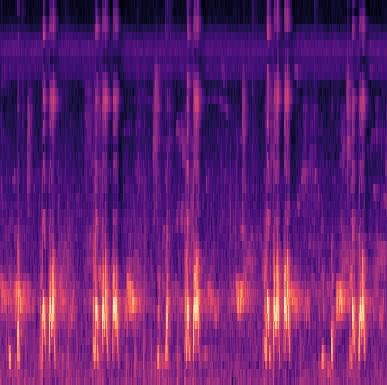
\includegraphics[width=0.4\textwidth]{images/koel_mel_spectrogram.jpg}
            \caption{Mel Spectrogram image for a sample audio}
            \label{fig:mel_spectrogram_sample}
      \end{figure}

      \newpage
      
      \subsection{Mel-Frequency Cepstral Coefficients (MFCC)}
      MFCCs are coefficients that collectively describe the short-term power spectrum
      of a sound signal. The process of obtaining MFCCs involves several steps:
      \begin{figure}[h!]
            \centering
            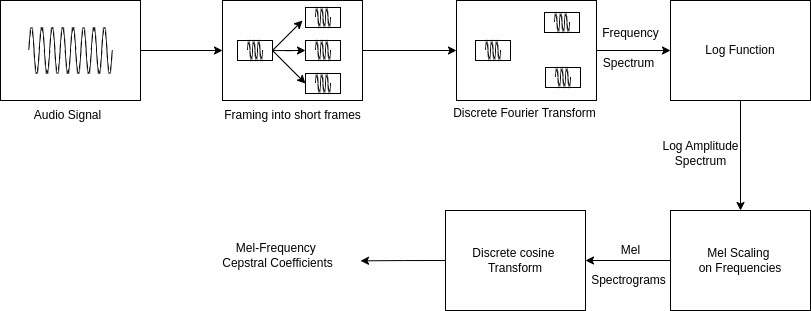
\includegraphics[scale=0.5]{images/MFCC.jpg}
            \caption{Feature Extraction Using Spectrogram and
                  MFCC}%\label{fig:fig1}
      \end{figure}
      
      \begin{enumerate}
            \item \textbf{Framing:} Divide the audio signal into short frames.
            \item \textbf{Discrete Fourier Transform (DFT):} Convert each frame to the
                  frequency domain.
                  \begin{eqnarray}
                        X(k) = \sum_{n=0}^{N-1} x(n) \cdot e^{-j \frac{2\pi}{N} kn}
                  \end{eqnarray}

            \item \textbf{Log Function:} Apply a logarithm to the amplitude spectrum.
                  \begin{eqnarray}
                        S_{\text{log}}(k) = \log(|X(k)|)
                  \end{eqnarray}

            \item \textbf{Mel-Scaling:} Map the frequencies to the Mel scale, which
                  better represents how humans perceive sound.
                  \begin{eqnarray}
                        f_{\text{mel}} = 2595 \cdot \log_{10}(1 + \frac{f}{700})
                  \end{eqnarray}

            \item \textbf{Discrete Cosine Transform (DCT):} Convert the Mel spectrum to
                  the cepstral domain, yielding the MFCC features.
                  \begin{eqnarray}
                        C(n) = \sum_{k=0}^{K-1} S_{\text{mel}}(k) \cdot \cos \left(
                        \frac{\pi n (k+0.5)}{K} \right)
                  \end{eqnarray}

      \end{enumerate}

      \begin{figure}[h!]
            \centering
            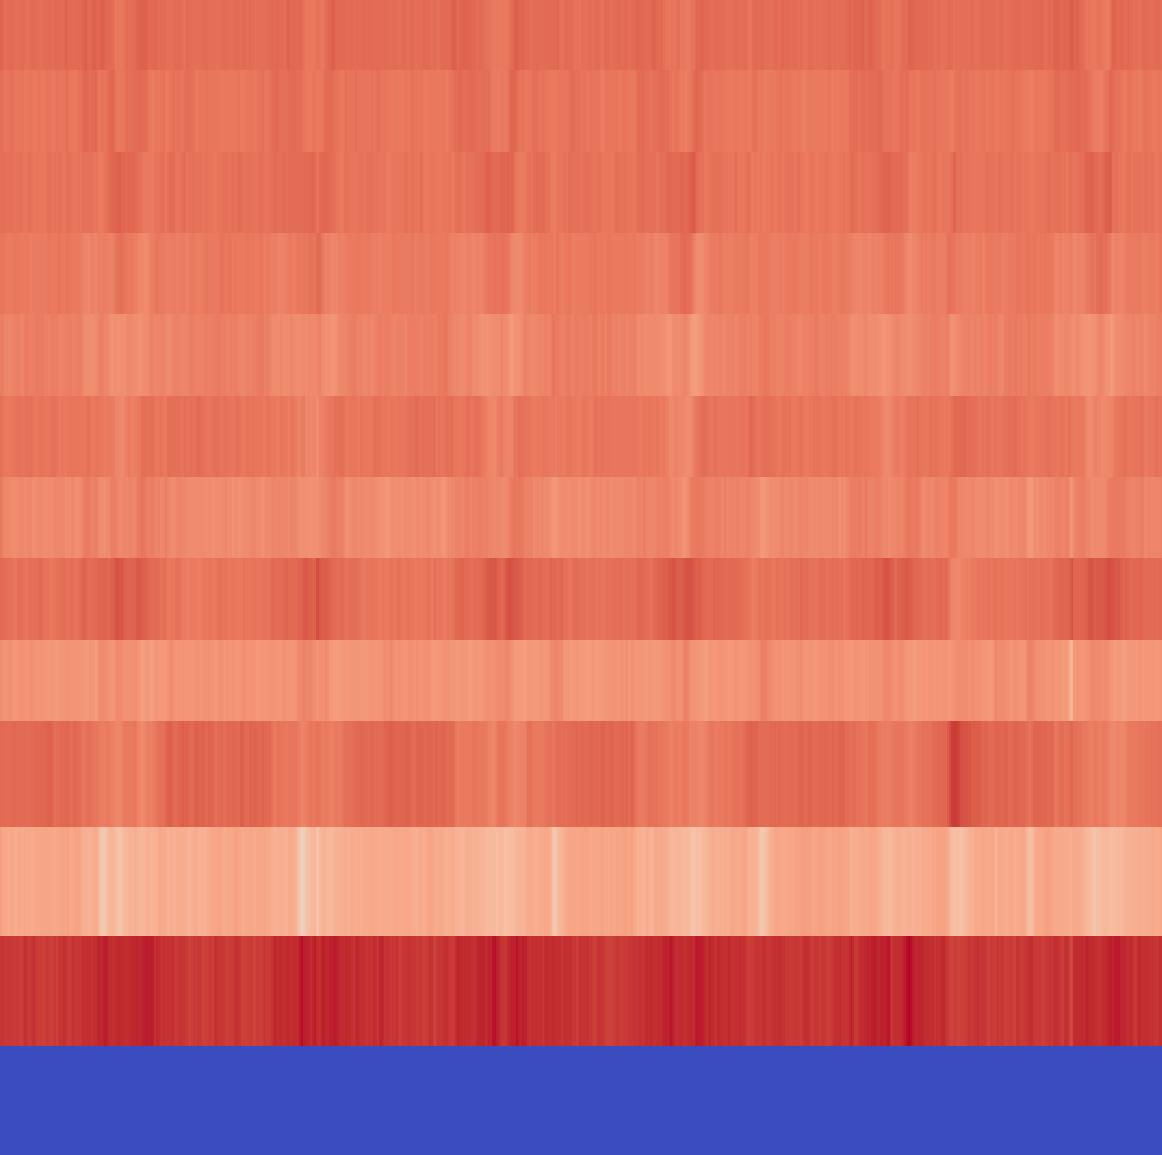
\includegraphics[width=0.4\textwidth]{images/koel_mfcc.jpg}
            \caption{MFCC image for a sample audio}
            \label{fig:mfcc_sample}
      \end{figure}
      


% Genetic Algorithm
\section{Hyperparameter Optimization using Genetic Algorithm}
Genetic algorithms are a powerful method for optimizing hyperparameters
in machine learning models. Genetic Algorithm have proven to significantly
improve the performance metrics of the CNN model instead of using hand tuned
approach for hyperparameters. This section outlines the steps involved in using
GAs for hyperparameter optimization\cite{9058307}.
\begin{itemize}
      \item \textbf{Encoding the Hyperparameters}
            \begin{itemize}
                  \item Hyperparameters are represented as a chromosome, where each hyperparameter is a
                        gene in the chromosome.
                  \item For example, in a neural network, a chromosome might include genes for the
                        learning rate, number of layers, number of neurons per layer, and activation
                        functions.
            \end{itemize}

      \item \textbf{Initial Population}
            \begin{itemize}
                  \item An initial population of chromosomes is generated randomly, with each
                        chromosome representing a different set of hyperparameters.
            \end{itemize}

      \item \textbf{Fitness Function}
            \begin{itemize}
                  \item A fitness function is defined to evaluate the performance of each set of
                        hyperparameters.
                  \item This typically involves training the model with the given hyperparameters and
                        measuring its performance on a validation set.
            \end{itemize}

      \item \textbf{Selection}
            \begin{itemize}
                  \item Selection involves choosing the best-performing chromosomes to serve as parents
                        for the next generation.
                  \item Various selection methods can be employed, such as tournament selection,
                        roulette wheel selection, or rank-based selection.
            \end{itemize}
            
      \item \textbf{Crossover (Recombination)}
            \begin{itemize}
                  \item Crossover combines pairs of parent chromosomes to produce offspring for the
                        next generation.
                  \item This is done by swapping segments of parent chromosomes to create new
                        chromosomes, thereby combining features of both parents.
            \end{itemize}

      \item \textbf{Mutation}
            \begin{itemize}
                  \item Mutation introduces random changes to some of the genes in the offspring
                        chromosomes.
                  \item This helps maintain genetic diversity in the population and allows the
                        algorithm to explore a broader search space.
            \end{itemize}

      \item \textbf{Replacement}
            \begin{itemize}
                  \item The current population is partially or entirely replaced with the new
                        generation of chromosomes, ensuring that better solutions are carried forward
                        while allowing for exploration of new possibilities.
            \end{itemize}

      \item \textbf{Termination}
            \begin{itemize}
                  \item The process of selection, crossover, mutation, and replacement is repeated
                        until a termination criterion is met.
                  \item This could be a set number of generations, convergence of fitness scores, or
                        achieving a satisfactory performance level.
            \end{itemize}

      \item \textbf{Best Solution}
            \begin{itemize}
                  \item The best chromosome at the end of the process represents the optimal or
                        near-optimal set of hyperparameters for the model.
            \end{itemize}
\end{itemize}
\newpage

\chapter{Results and Analysis}
In the course of our project on Bird Species Classification from Audio, we have
accomplished several key tasks to progress our analysis and model development:

\section{Bird Sound Detection}

Figure \ref{fig:training_curves} shows the training progress over 15 epochs. The model shows consistent improvement in both accuracy and loss metrics during training and validation phases.

\begin{figure}[h!]
      \centering
      \begin{subfigure}{\textwidth}
            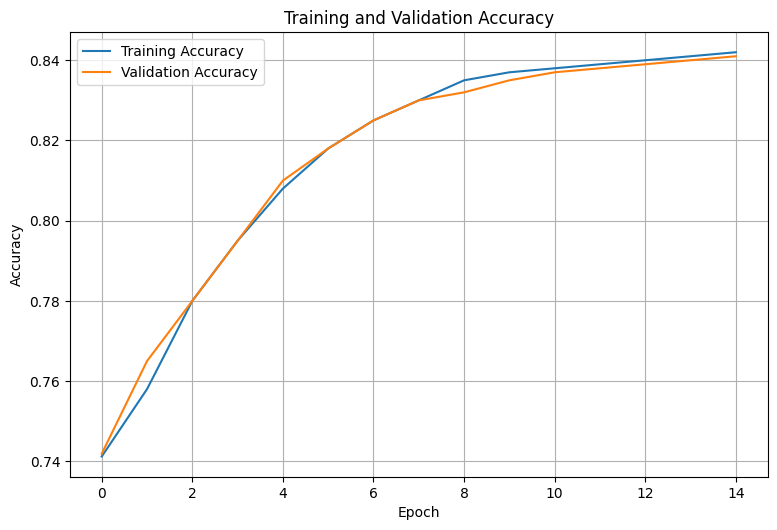
\includegraphics[width=\textwidth]{images/det_acc.png}
            \caption{Accuracy curves}
      \end{subfigure}
      \begin{subfigure}{\textwidth}
            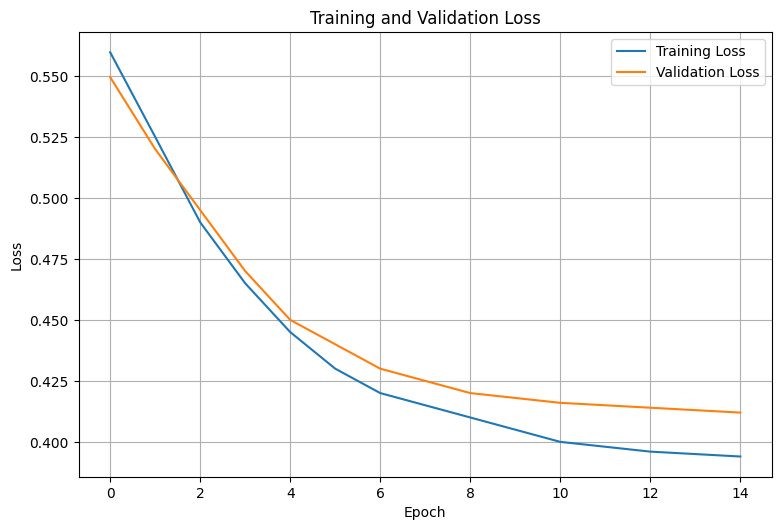
\includegraphics[width=\textwidth]{images/det_loss.png}
            \caption{Loss curves}
      \end{subfigure}
      \caption{Training and validation curves for Bird Sound Detection Model}
      \label{fig:training_curves}
\end{figure}

The training process exhibited steady improvement, with the model achieving final metrics of:
\begin{itemize}
      \item Training accuracy: \textbf{84.20\%} and validation accuracy: \textbf{84.10\%}
            \item Training loss: \textbf{0.394} and validation loss: \textbf{0.412}
            \item Training F1-score: \textbf{0.585} and validation F1-score: \textbf{0.615}
      \end{itemize}

The close alignment between training and validation metrics indicates good generalization without overfitting. The loss curves show consistent convergence, while accuracy and F1-scores demonstrate steady improvement throughout the training process.

The confusion matrix in Figure \ref{fig:Confusion Matrix for Detection Model} shows the classification performance on the test dataset. From the total of \textbf{1621} samples, the model correctly classified \textbf{621} samples as non-bird sounds (True Negatives) and \text{680} samples as bird sounds (True Positives). There were 107 false positives and \textbf{160} false negatives.
\begin{figure}[h!]
      \centering
      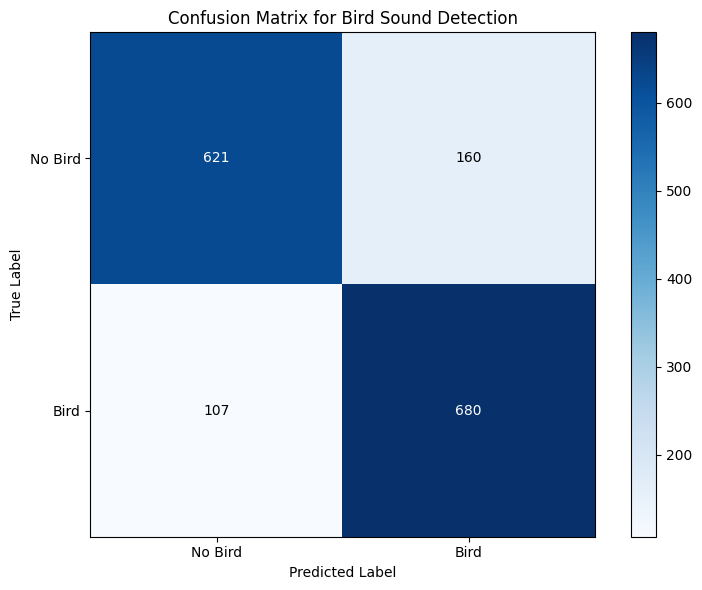
\includegraphics[scale=0.75]{images/detection_cm.png}
      \caption{Confusion Matrix for Bird Sound Detection Model}
      \label{fig:Confusion Matrix for Detection Model}
\end{figure}
The model performance metrics are summarized in Table \ref{tab:detection_metrics}.

\begin{table}[h]
      \centering
      \caption{Performance Metrics for Bird Sound Detection Model}
      \label{tab:detection_metrics}
      \begin{tabular}{|l|c|}
            \hline
            \textbf{Metric} & \textbf{Value (\%)} \\
            \hline
            Accuracy & 82.97 \\
            F1-score & 83.59 \\
            Precision & 80.95 \\
            Recall & 86.40 \\
            \hline
      \end{tabular}
\end{table}

Figure \ref{fig:ROC Curve} shows the Receiver Operating Characteristic (ROC) curve for the bird sound detection model. The curve illustrates the model's ability to discriminate between bird and non-bird sounds across different classification thresholds.
\begin{figure}[h!]
    \centering
    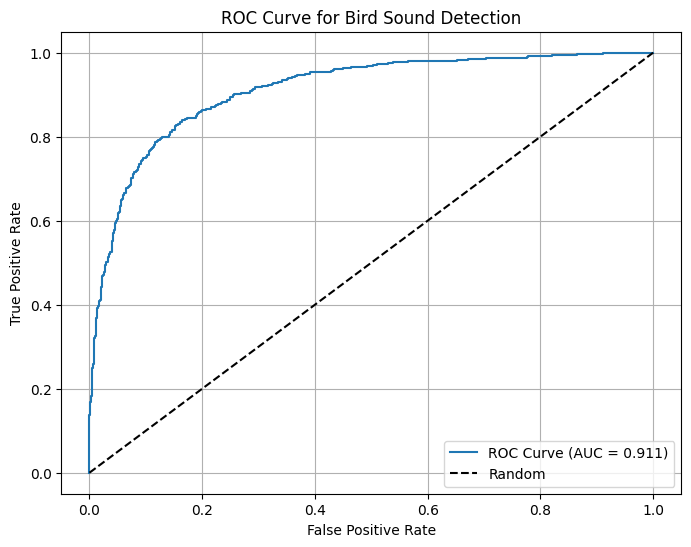
\includegraphics[scale=0.65]{images/detection_auc.png}
    \caption{ROC Curve of the detection model}
    \label{fig:ROC Curve}
\end{figure}

The Area Under the Curve (AUC) score of \textbf{0.911} indicates excellent discriminative ability, as it is significantly higher than the random chance baseline of \textbf{0.5}.
\section{Bird Species Classification}
The below figures show the outcomes of Bird Species Classification based on two different architectures i.e CNN-LSTM and EfficientNetB3, evaluated on our dataset of 41 bird species.

\subsection{Classification using CNN-LSTM}
The CNN-LSTM model achieved an accuracy of \textbf{74.73\%} with a cross-entropy loss of \textbf{1.0171} across all 41 bird species. The confusion matrix shows stronger diagonal elements indicating good classification ability for most species, though there is some confusion between similar-sounding birds.
\begin{figure}[h!]
      \centering
      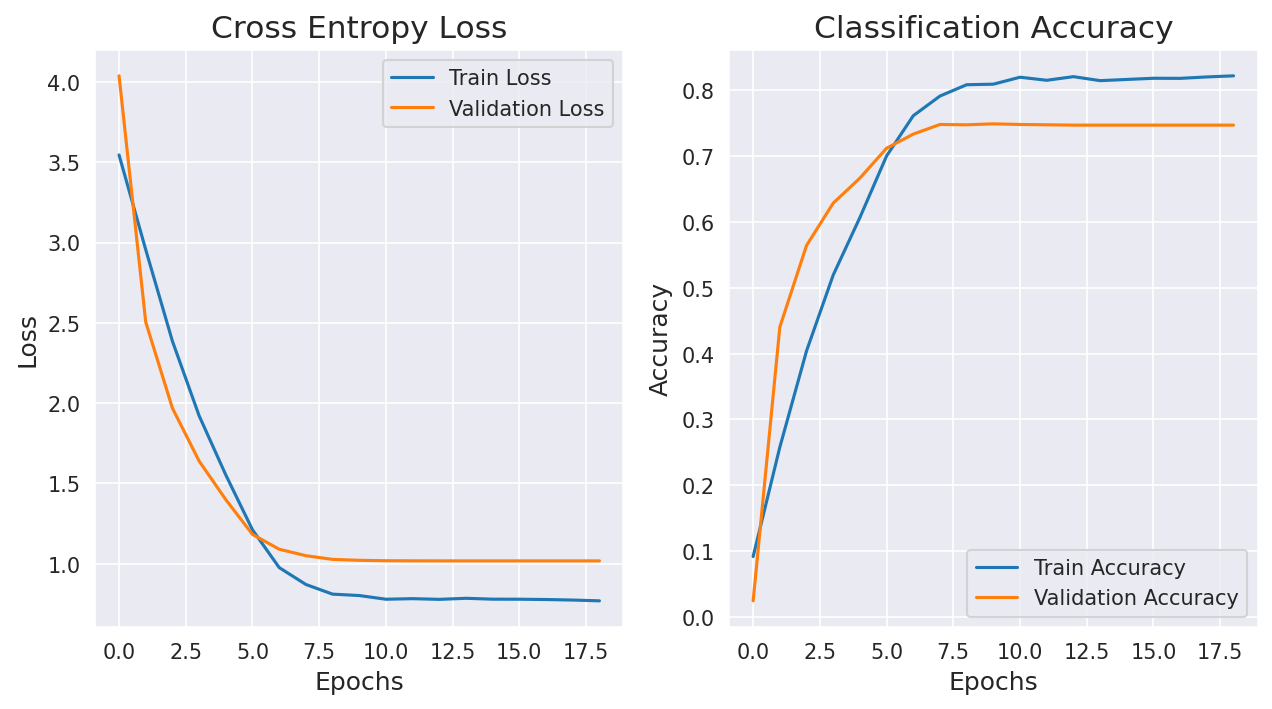
\includegraphics[scale=0.6]{images/cnn_lstm_evaluation.png}
      \caption{CNN-LSTM Model Evaluation}
  \end{figure}
      The training and validation curves show the model achieved a training accuracy of \textbf{80.76\%} and validation accuracy of \textbf{74.73\%}, with corresponding losses of \textbf{0.8025} and \textbf{1.0171} respectively.
\newpage
\begin{figure}[h!]
      \centering
      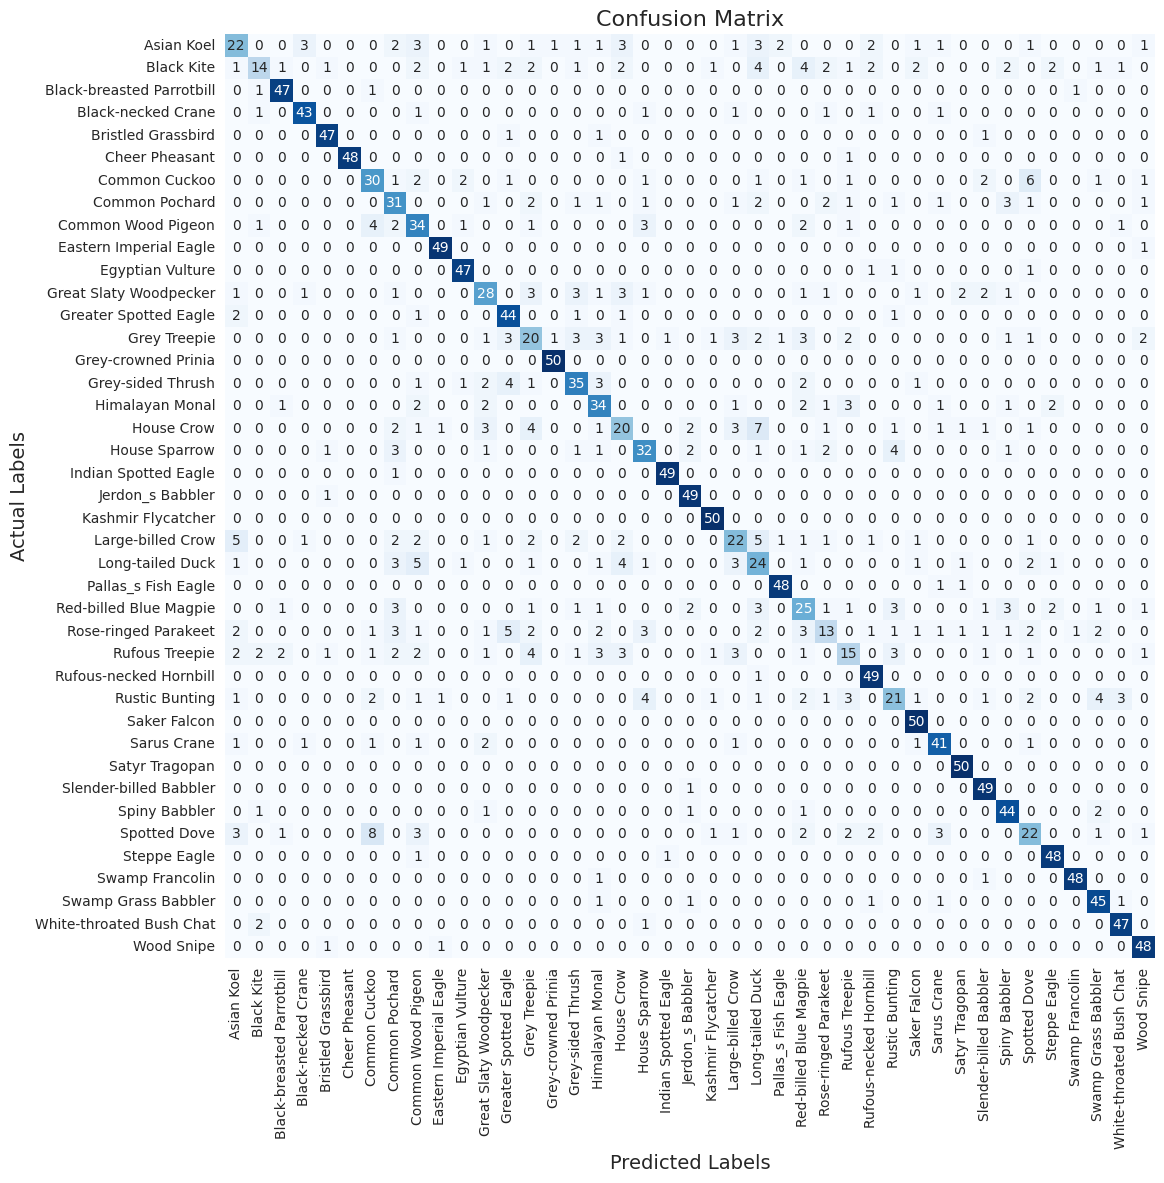
\includegraphics[scale=0.5]{images/cnn_lstm_confusion_matrix.png}
      \caption{CNN-LSTM Confusion Matrix}
  \end{figure}
The confusion matrix visualizes the model's predictions across all 41 classes, with darker diagonal elements indicating correct classifications and lighter off-diagonal elements showing misclassifications between species.

\begin{figure}[h!]
      \centering
      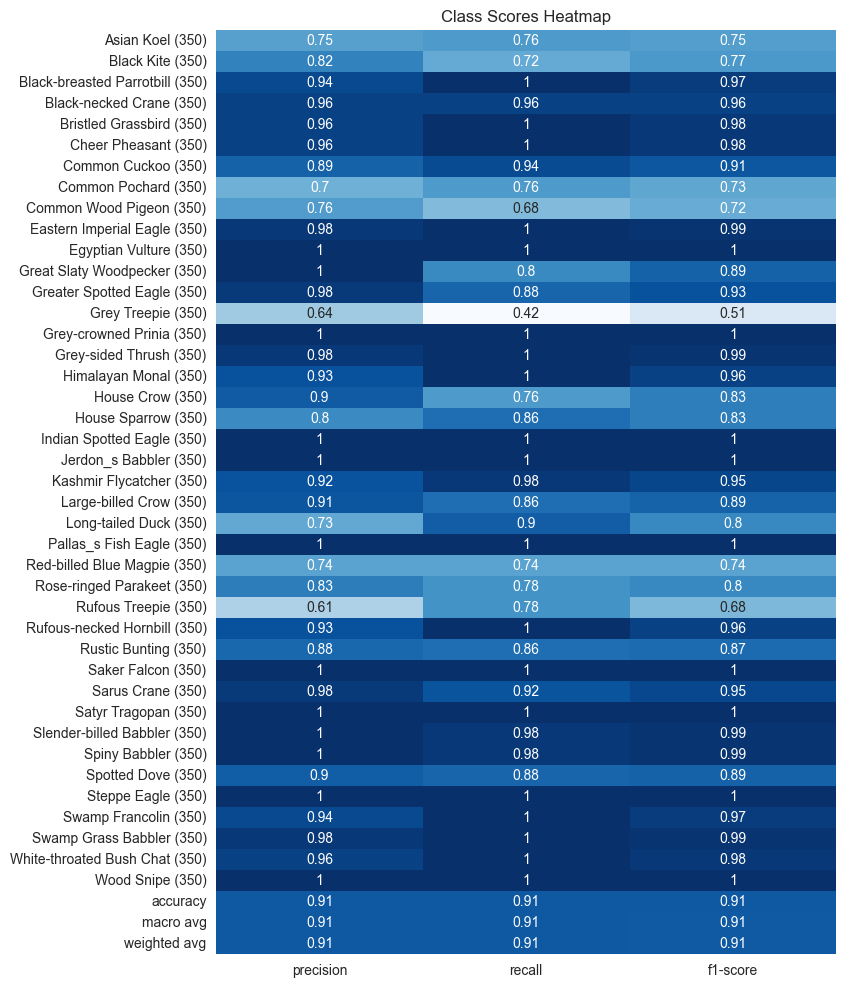
\includegraphics[scale=0.6]{images/efficientNet_classification_report.png}
      \caption{CNN-LSTM Classification Report}
  \end{figure}
  \newpage
The classification report shows detailed metrics for each species, with an average precision of \textbf{73\%}, recall of \textbf{75\%}, and F1-score of \textbf{73\%} across all classes.


\newpage
\subsection{Classification using EfficientNetB3}
The EfficientNetB3 model demonstrated superior performance with an accuracy of \textbf{90.73\%} with a cross-entropy loss of \textbf{0.4154}, significantly outperforming the CNN-LSTM architecture. The confusion matrix reveals excellent discrimination ability across most species, with minimal misclassifications between different bird calls.

\begin{figure}[h!]
            \centering
            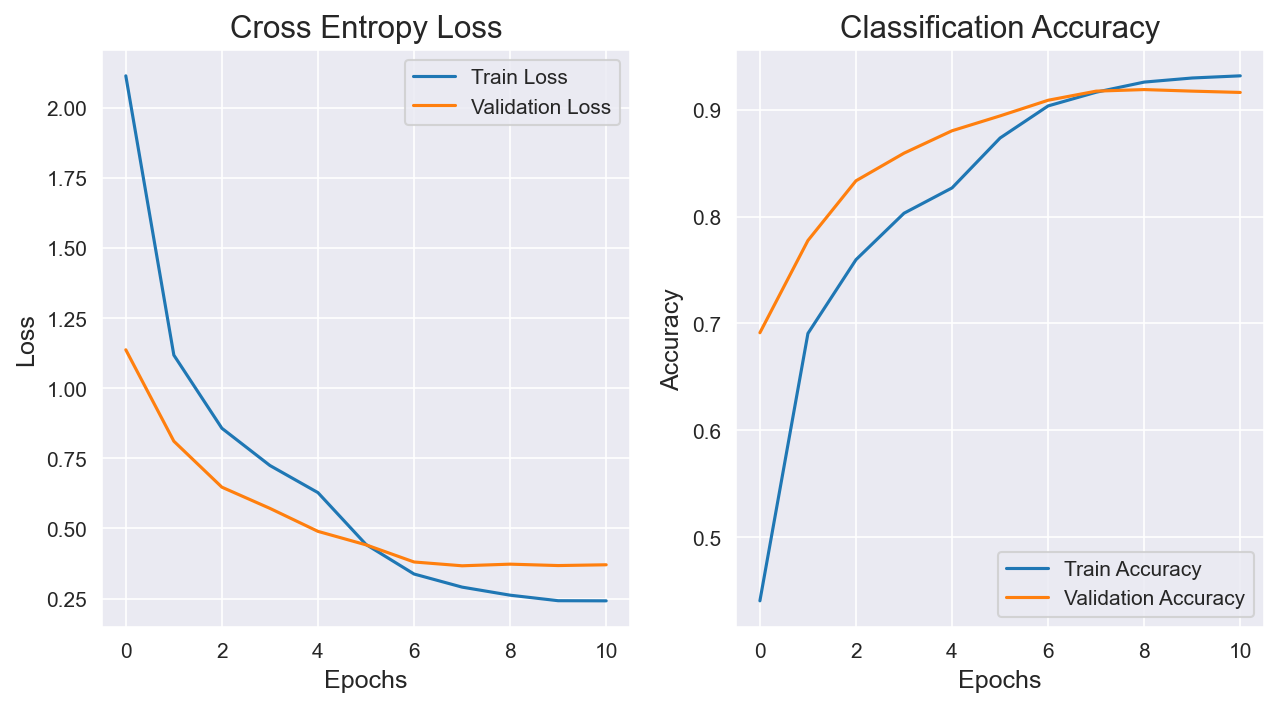
\includegraphics[scale=0.6]{images/efficientNet_evaluation.png}
            \caption{EfficientNetB3 Model Evaluation}
      \end{figure}
The training and validation curves demonstrate strong performance with a training accuracy of \textbf{93.32\%} and validation accuracy of \textbf{91.61\%}, while maintaining low loss values of \textbf{0.2336} and \textbf{0.3706} respectively.
\newpage
\begin{figure}[h!]
            \centering
            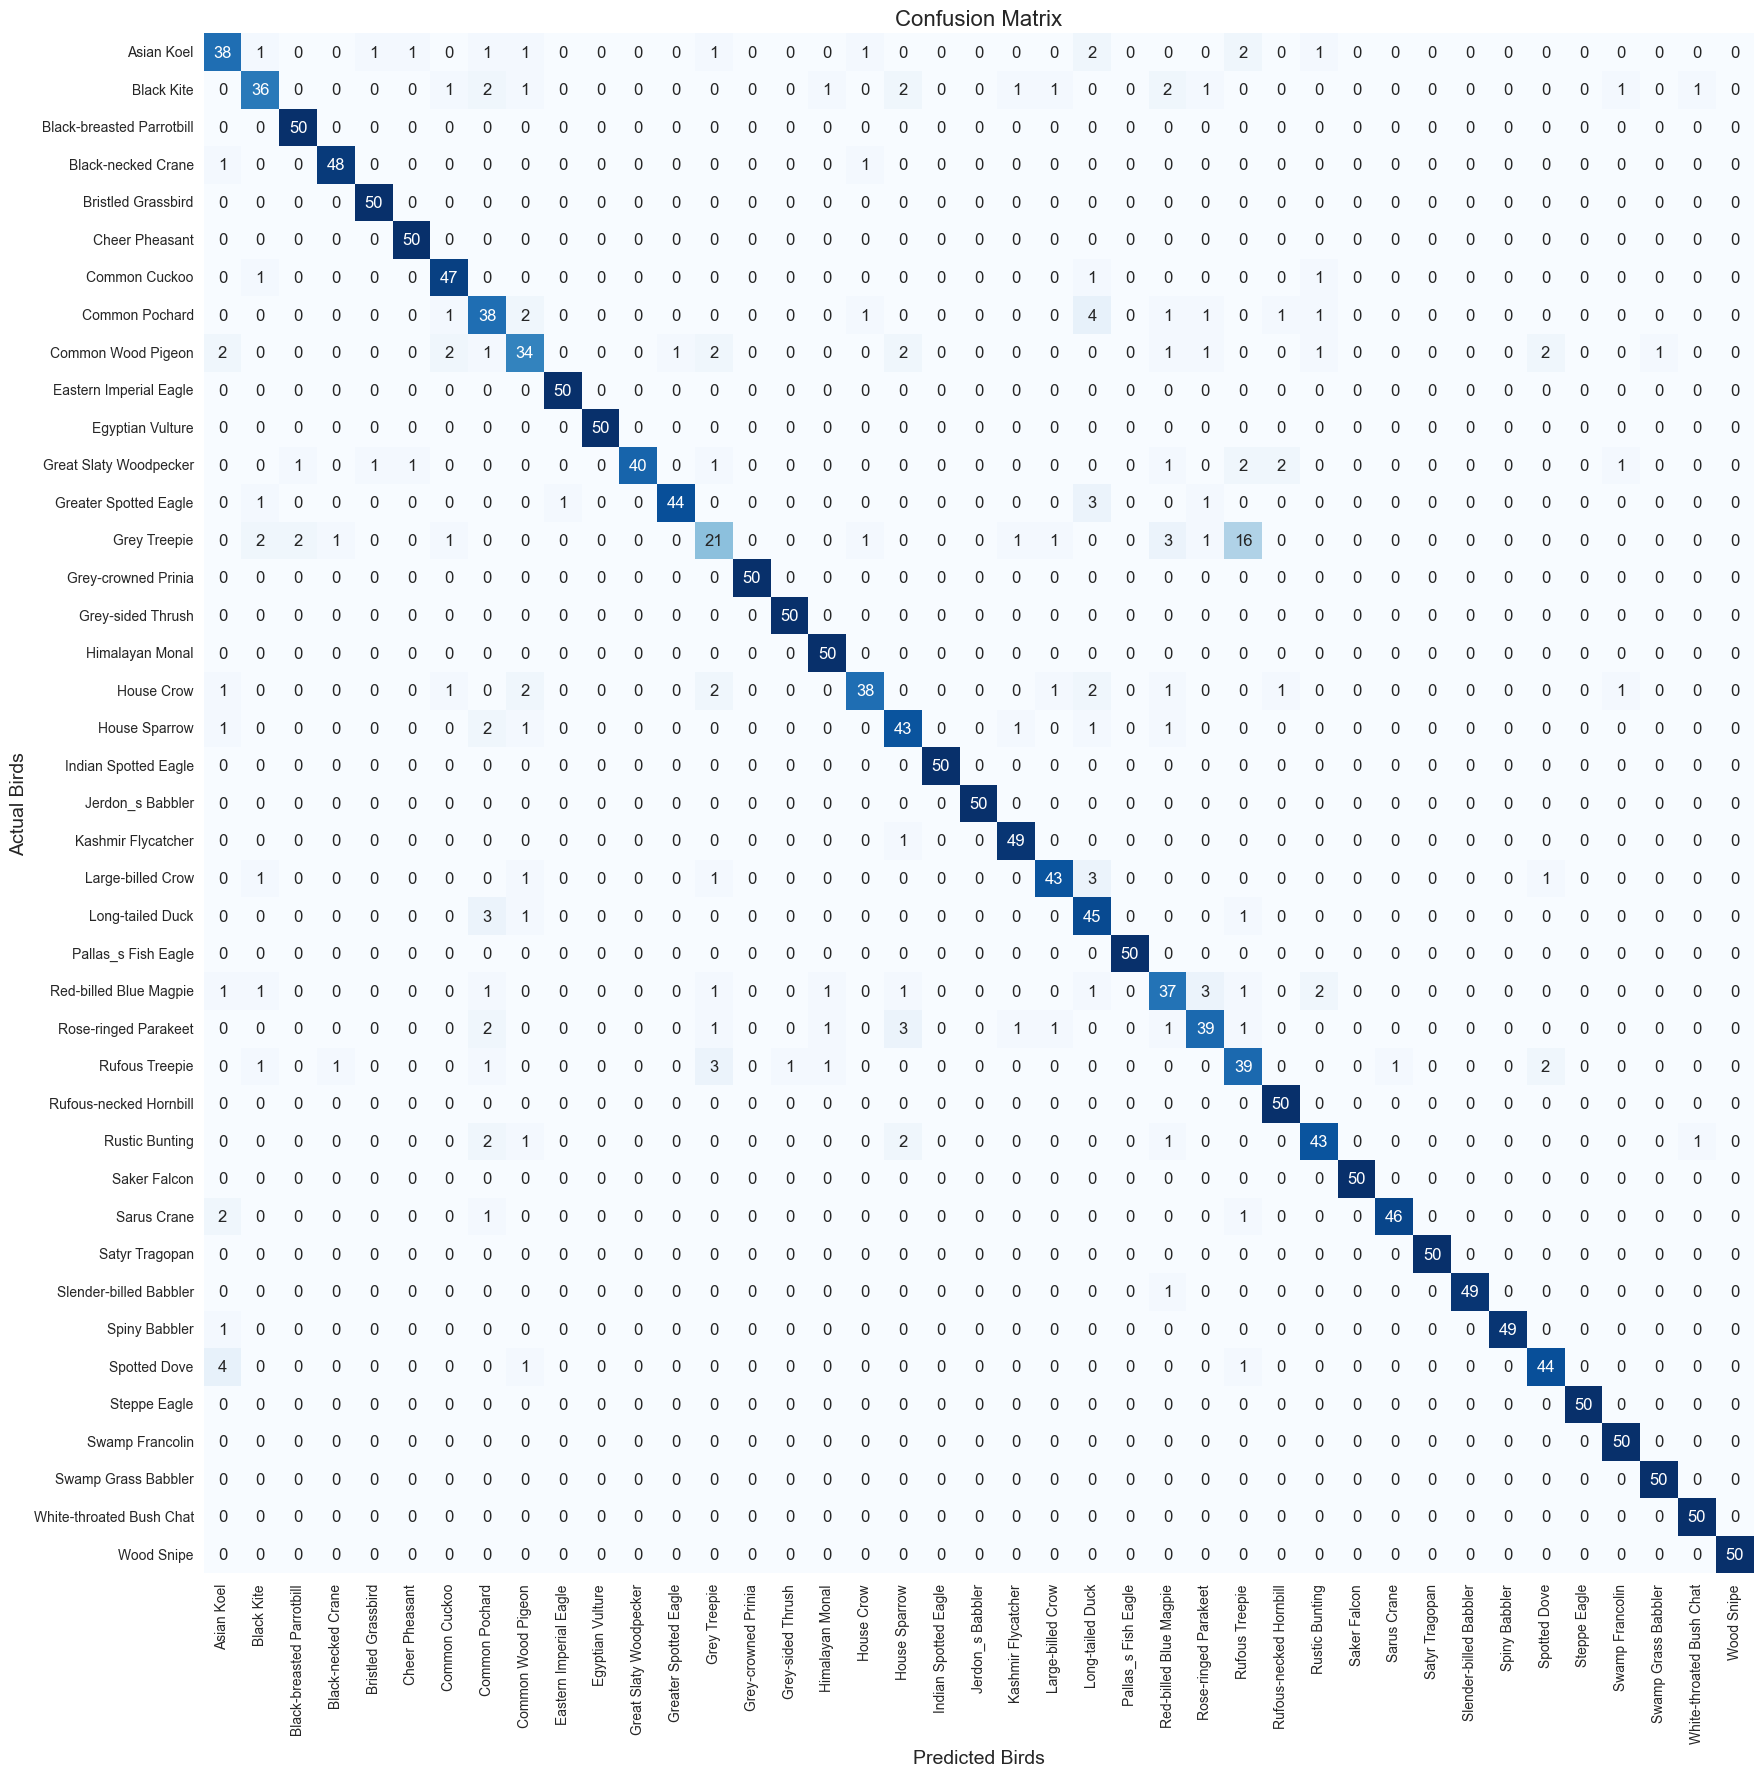
\includegraphics[scale=0.35]{images/efficientNet_confusion_matix.png}
            \caption{EfficientNetB3 Confusion Matrix}
      \end{figure}
      The confusion matrix shows strong diagonal elements indicating excellent classification accuracy across most species, with minimal confusion between different bird calls.
\newpage

\begin{figure}[h!]
            \centering
            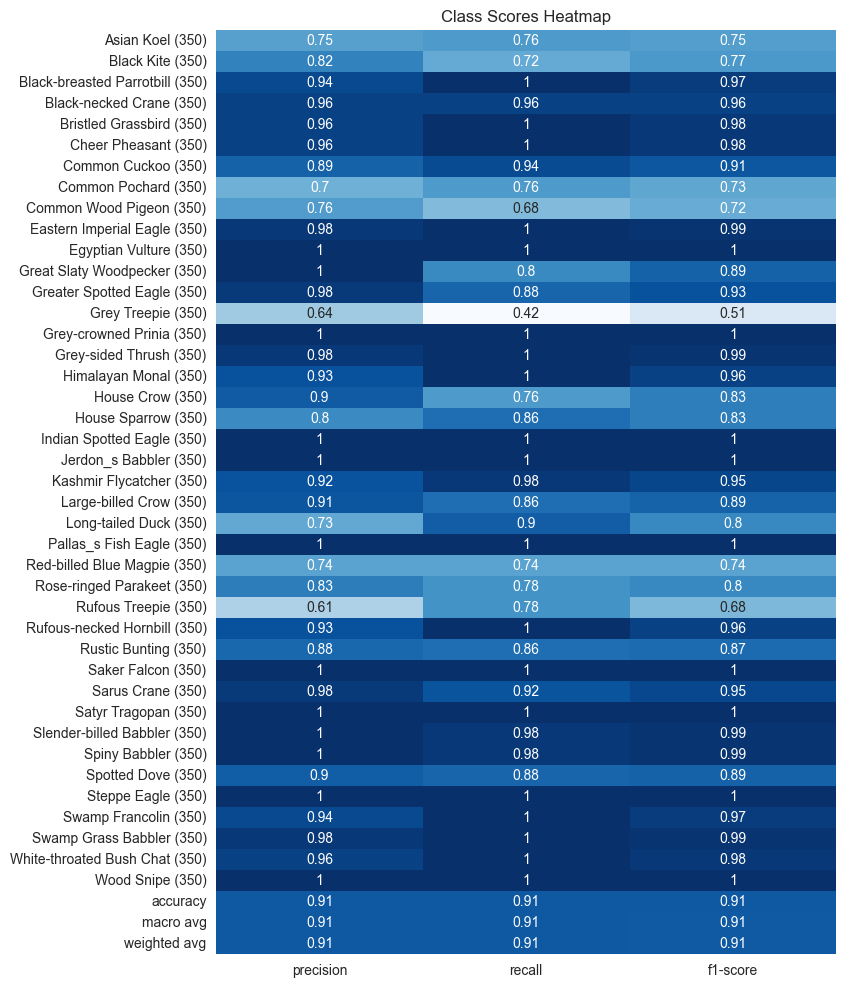
\includegraphics[scale=0.6]{images/efficientNet_classification_report.png}
            \caption{EfficientNetB3 Classification Report}
      \end{figure}
The classification report shows detailed metrics for each species, with an average precision, recall and f1-score of \textbf{91\%} across all classes.

\newpage
\section{Hyperparameter Optimization Using Genetic Algorithim}
To optimize the performance of our model, we used genetic algorithm for
hyperparameter tuning. This approach helped us systematically explore and
identify the most effective hyperparameter settings for our model, including network architecture parameters like
learning rates, batch sizes, images sizes, dropout and others. The genetic
algorithm enabled a more efficient and comprehensive search for optimal
configurations.
\subsection{Hyperparameters for CNN-LSTM}
For the CNN-LSTM model, GA was applied to tune  hyperparameters that impact both convolutional feature extraction and model efficiency. The key hyperparameters optimized includes Batch Size, Learning Rate, Number of Epochs, Dropout Rate, LSTM Units and Dense Units.
The genetic algorithm was executed over multiple generations, evolving hyperparameter configurations towards optimal performance.

\subsubsection{Hyperparameter Search Space}
The genetic algorithm optimized the following hyperparameters:

\begin{table}[h]
    \centering
    \begin{tabular}{|l|c|}
        \hline
        \textbf{Hyperparameter} & \textbf{Search Values} \\
        \hline
        Batch Size & \{16, 32, 64\} \\
        Learning Rate & \{1e-4, 1e-4, 1e-3\} \\
        Epochs & \{20, 30, 40\} \\
        Dropout Rate & \{0.3, 0.4, 0.5\} \\
        LSTM Units & \{64, 128, 256\} \\
        Dense Units & \{64, 128, 256\} \\
        \hline
    \end{tabular}
    \caption{Hyperparameter search space for CNN-LSTM}
    \label{tab:search_space}
\end{table}

\subsubsection{Genetic Algorithm Process}
The GA followed an evolutionary approach, iterating over multiple generations to refine hyperparameters. The process consisted of:

\begin{itemize}
    \item \textbf{Population Size:} 3 (each generation consists of 3 hyperparameter sets)
    \item \textbf{Generations:} 2 (iterative evolution of hyperparameters)
    \item \textbf{Mutation Rate:} 10\% (randomly modifying one parameter)
    \item \textbf{Crossover:} Parents were selected based on validation accuracy, and offspring were created by combining their hyperparameters.
\end{itemize}
\subsubsection{Results}
Over two generations, the algorithm refined hyperparameters, improving model accuracy and minimizing overfitting. The following images illustrate training and validation performance trends for different hyperparameter configurations across generations.

The Following Graphs shows the training and validation accuracies and loss for the respective hyperparameters used for CNN-LSTM.\\
\begin{figure}[h!]
      \centering
      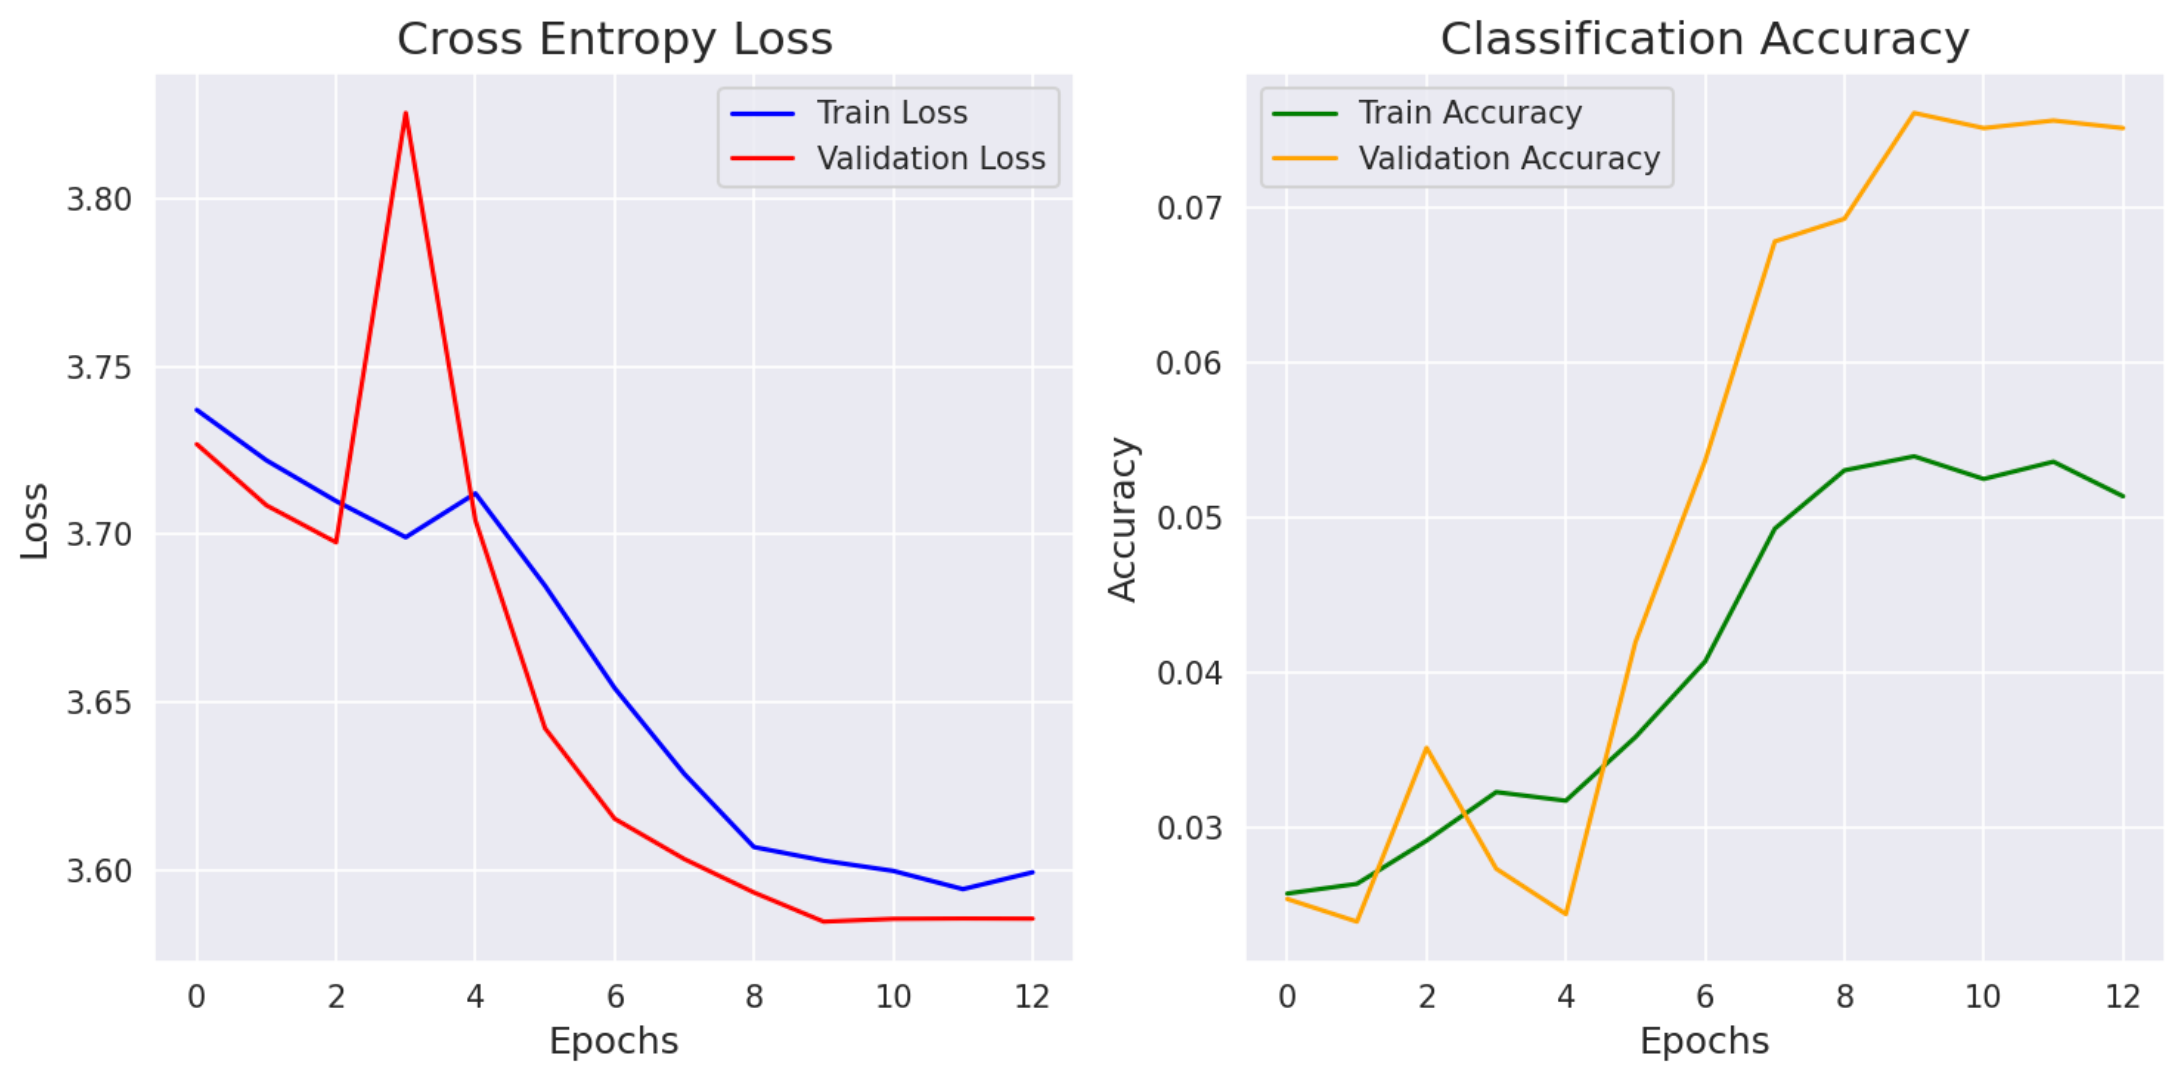
\includegraphics[scale=0.18]{images/GA_CNN_LSTM_1.png}
      \caption{Accuracy and Loss for CNN-LSTM in generation 1}
  \end{figure}
\begin{figure}[h!]
      \centering
      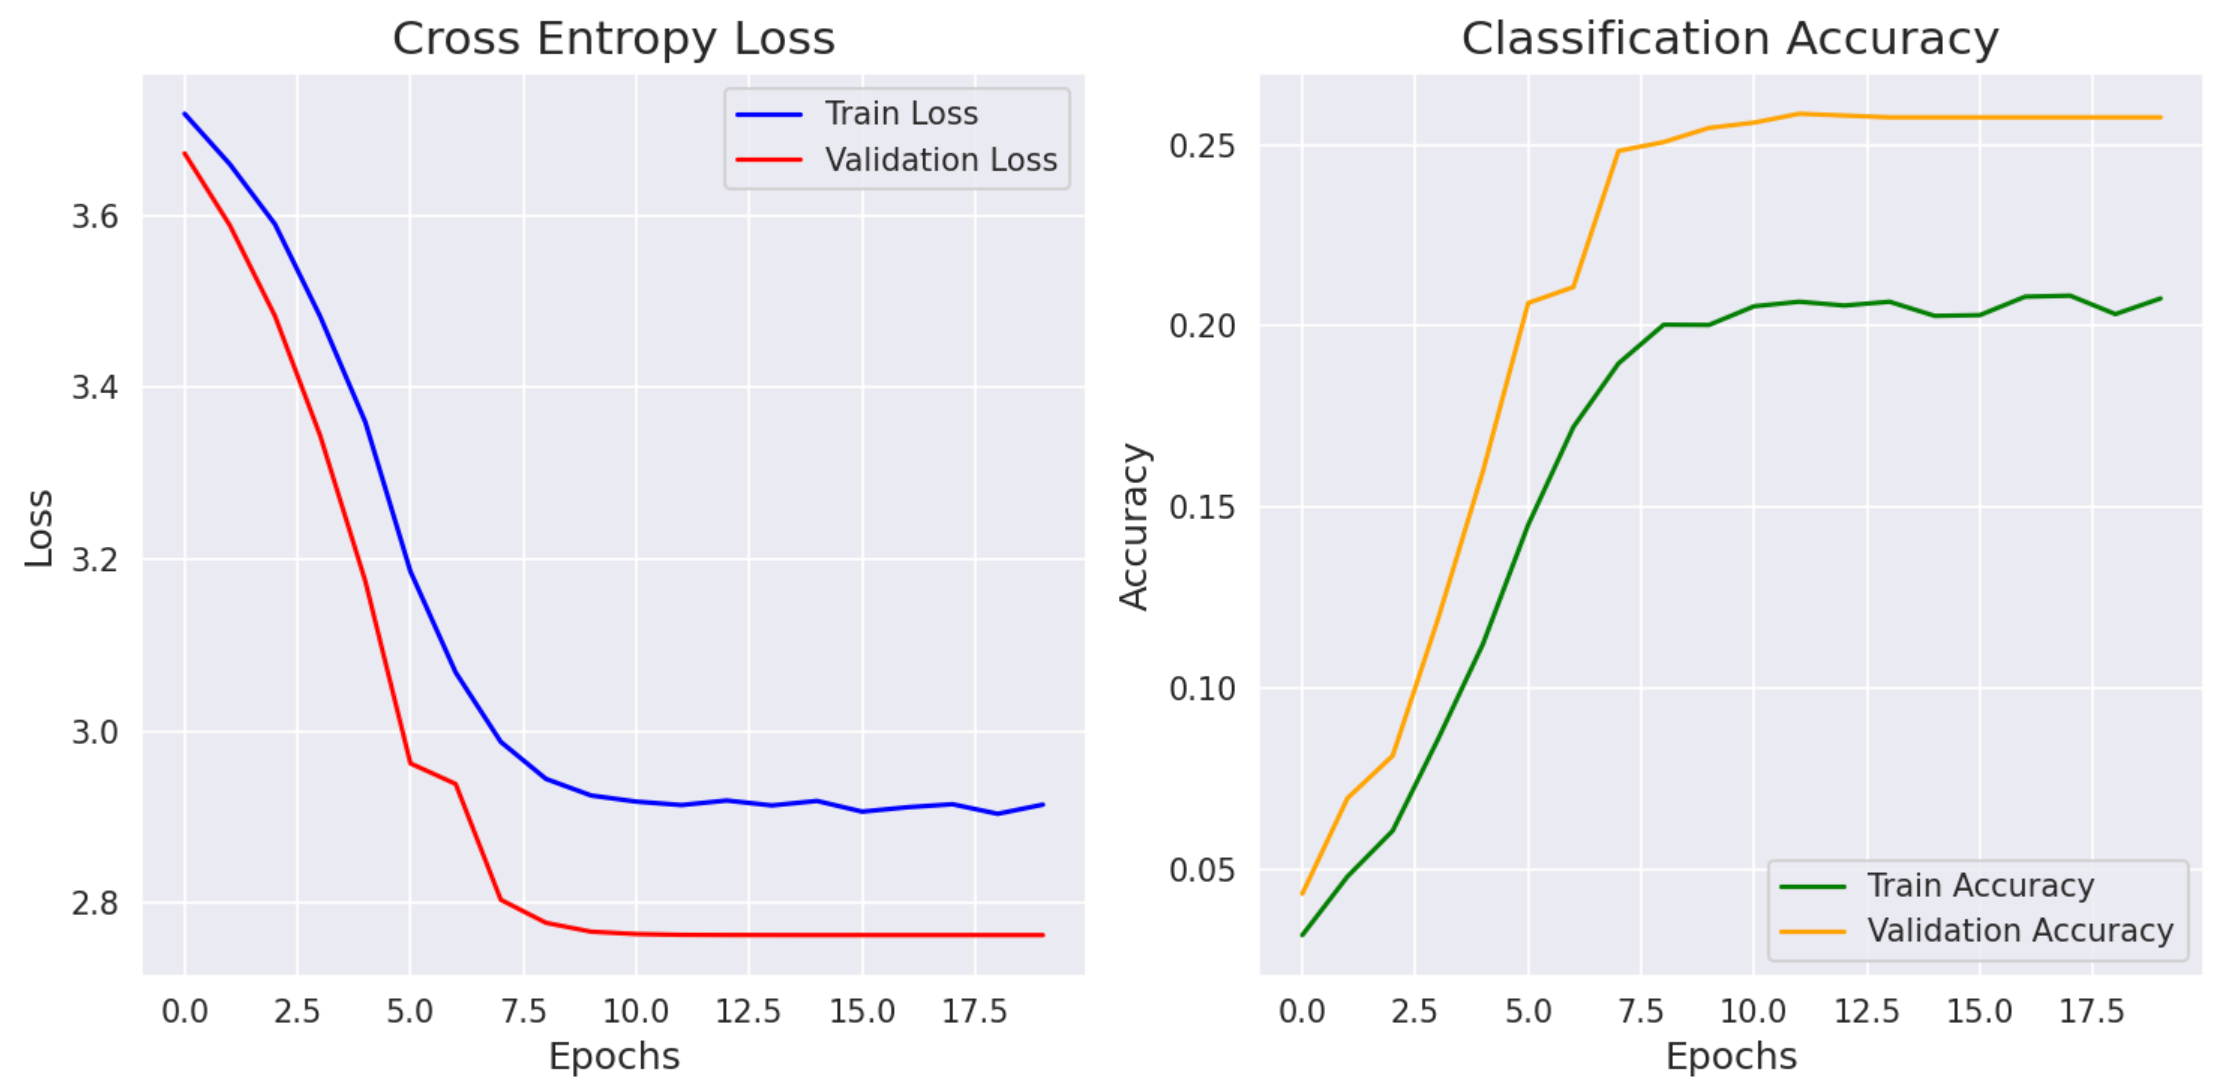
\includegraphics[scale=0.18]{images/GA_CNN_LSTM_2.png}
      \caption{Accuracy and Loss for CNN-LSTM in generation 2}
  \end{figure}
  \newpage
\begin{figure}[h!]
      \centering
      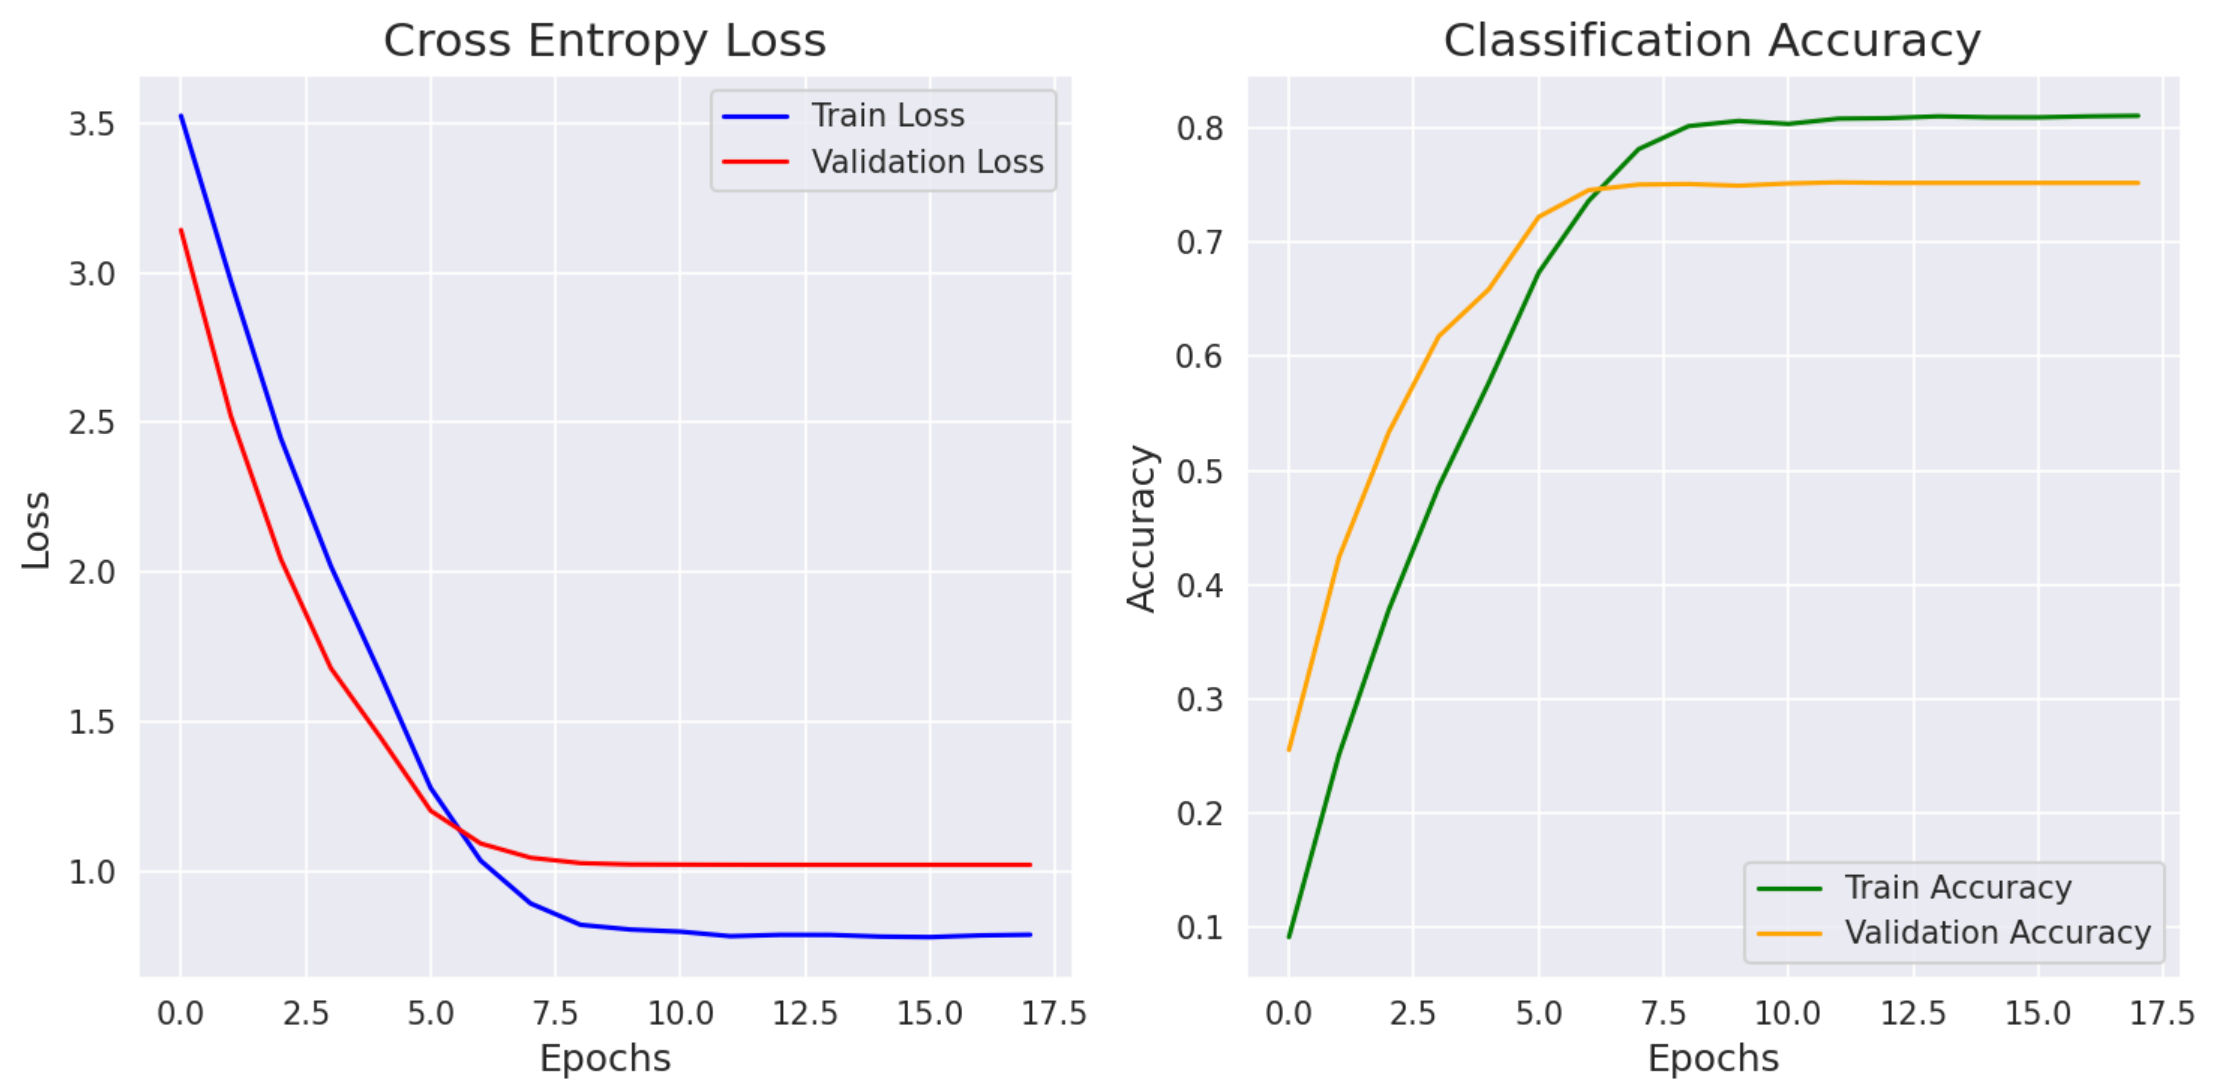
\includegraphics[scale=0.18]{images/GA_CNN_LSTM_3.png}
      \caption{Accuracy and Loss for CNN-LSTM in generation 3}
  \end{figure}
\begin{figure}[h!]
      \centering
      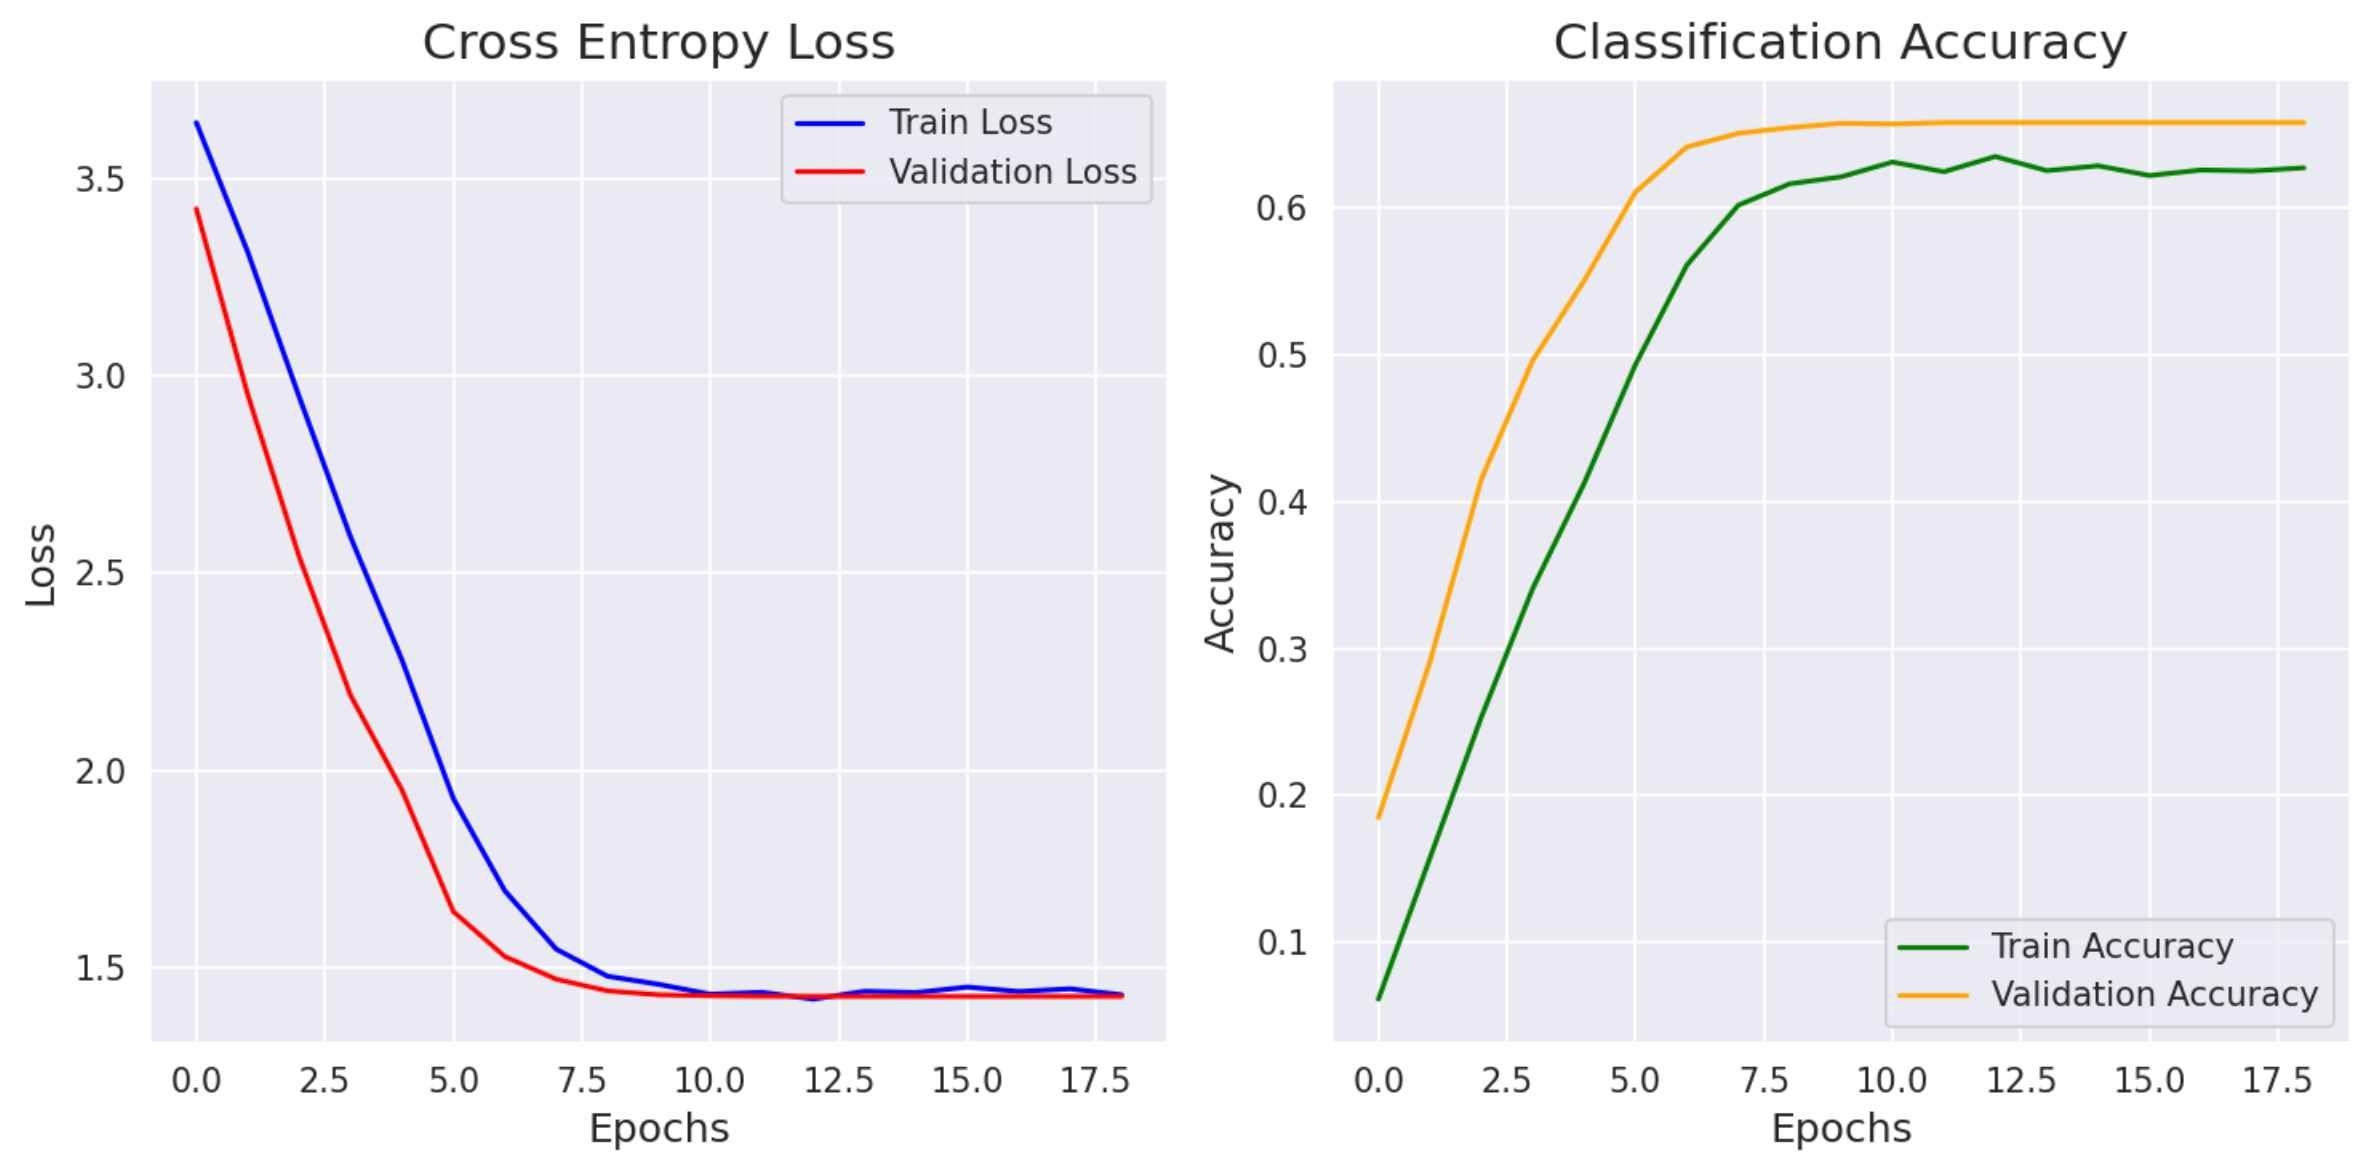
\includegraphics[scale=0.18]{images/GA_CNN_LSTM_4.png}
      \caption{Accuracy and Loss for CNN-LSTM in generation 4}
  \end{figure}
\begin{figure}[h!]
      \centering
      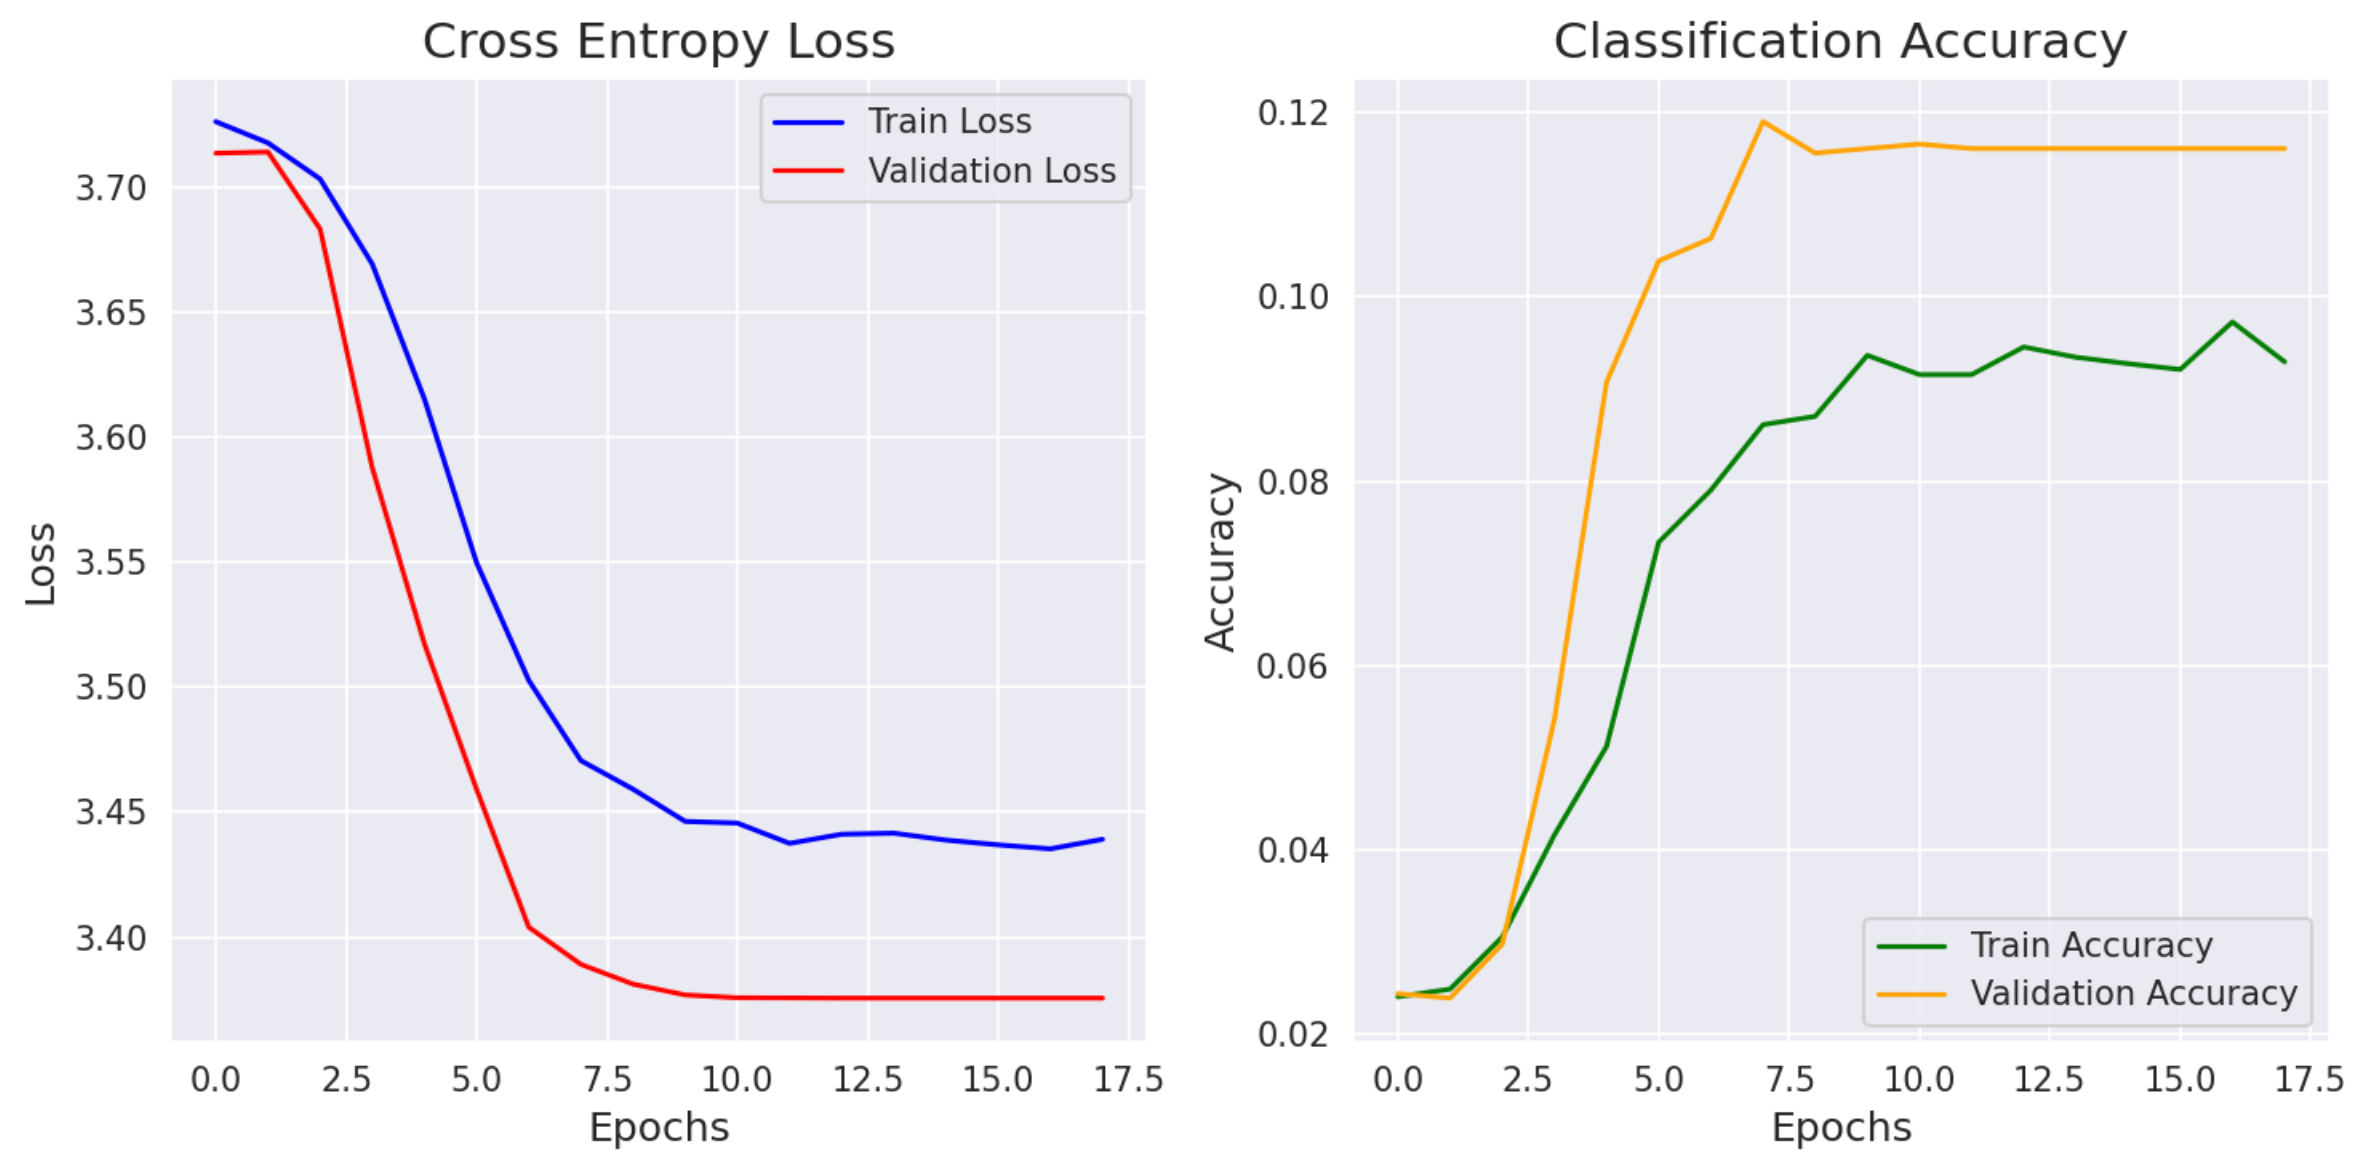
\includegraphics[scale=0.18]{images/GA_CNN_LSTM_5.png}
      \caption{Accuracy and Loss for CNN-LSTM in generation 5}
  \end{figure}

\newpage
The following table demonstrates different hyperparameter configurations and their corresponding test accuracies.

\begin{table}[h!]
      \centering
      \resizebox{\textwidth}{!}{  % Automatically scale to fit
      \begin{tabular}{|c|c|c|c|c|c|c|c|}
          \hline
          \textbf{SN} & \textbf{Batch} & \textbf{LR} & \textbf{Epochs} & \textbf{Dropout} & \textbf{LSTM Units} & \textbf{Dense Units} & \textbf{Test Accuracy (\%)} \\
          \hline
          1 & 64  & 0.001  & 40  & 0.5  & 128  & 64  & 7.61 \\
          2 & 16  & 0.001  & 30  & 0.3  & 256  & 64  & 25.76 \\
          3 & 16  & 0.0001 & 20  & 0.3  & 256  & 64  & \textbf{75.17} \\
          4 & 16  & 0.0001 & 20  & 0.4  & 256  & 64  & 65.80 \\
          5 & 16  & 0.001  & 30  & 0.3  & 65   & 64  & 11.61 \\
          \hline
      \end{tabular}
      }
      \caption{Hyperparameter configurations and test accuracies for CNN-LSTM}
      \label{tab:cnn_lstm_results}
\end{table}


\subsubsection{Conclusion}
The best model achieved a Test Accuracy of \textbf{75.17\%} with a \textbf{Batch Size of 16}, \textbf{Learning Rate of 0.0001}, \textbf{Epochs = 20}, \textbf{Dropout Rate of 0.3}, \textbf{LSTM Units = 256}, and \textbf{Dense Units = 64}. These results highlight the effectiveness of the Genetic Algorithm in systematically optimizing hyperparameters, leading to improved learning efficiency and minimized overfitting.

% % Figure 
% \begin{figure}[h!]
%     \centering
%     \includegraphics[scale=0.18]{images/.png}
%     \caption{GA CNN-LSTM.}
% \end{figure}

\subsection{Hyperparameters for Efficient-Net}
For EfficientNet, GA was used to fine-tune hyperparameters that directly affect feature extraction and classification efficiency. The optimized parameters includes Batch Size, Learning Rate, Number of Epochs, Dropout Rate,Regularization and Dense Units.

\subsubsection{Hyperparameter Search Space}
The genetic algorithm optimized the following hyperparameters:
\begin{table}[h]
      \centering
      \begin{tabular}{|l|c|}
          \hline
          \textbf{Hyperparameter} & \textbf{Search Values} \\
          \hline
          Batch Size & \{4, 8, 16\} \\
          Image Size & \{(128, 128), (128, 128), (224, 224)\} \\
          Learning Rate & \{1e-4, 1e-4, 1e-3\} \\
          Epochs & \{20, 20, 20\} \\
          Dropout Rate & \{0.3, 0.2, 0.4\} \\
          L2 Regularization & \{1e-4, 1e-4, 1e-3\} \\
          \hline
      \end{tabular}
      \caption{Hyperparameter search space for the EfficientNetB3}
      \label{tab:search_space}
  \end{table}
  
\subsubsection{Genetic Algorithm Process}
The GA followed an evolutionary approach, iterating over multiple generations to refine hyperparameters. The process consisted of:

\begin{itemize}
    \item \textbf{Population Size:} 3 (each generation consists of 3 hyperparameter sets)
    \item \textbf{Generations:} 2 (iterative evolution of hyperparameters)
    \item \textbf{Mutation Rate:} 10\% (randomly modifying one parameter)
    \item \textbf{Crossover:} Parents were selected based on validation accuracy, and offspring were created by combining their hyperparameters.
\end{itemize}

\subsubsection{Results}
Over three generations, the algorithm refined hyperparameters, leading to improved validation accuracy. The following figures illustrate training and validation performance trends for different hyperparameter configurations across generations.

The Following Graphs shows the training and validation accuracies and loss for the respective hyperparameters used for EfficientNetB3.

\begin{figure}[htbp]
      \centering
      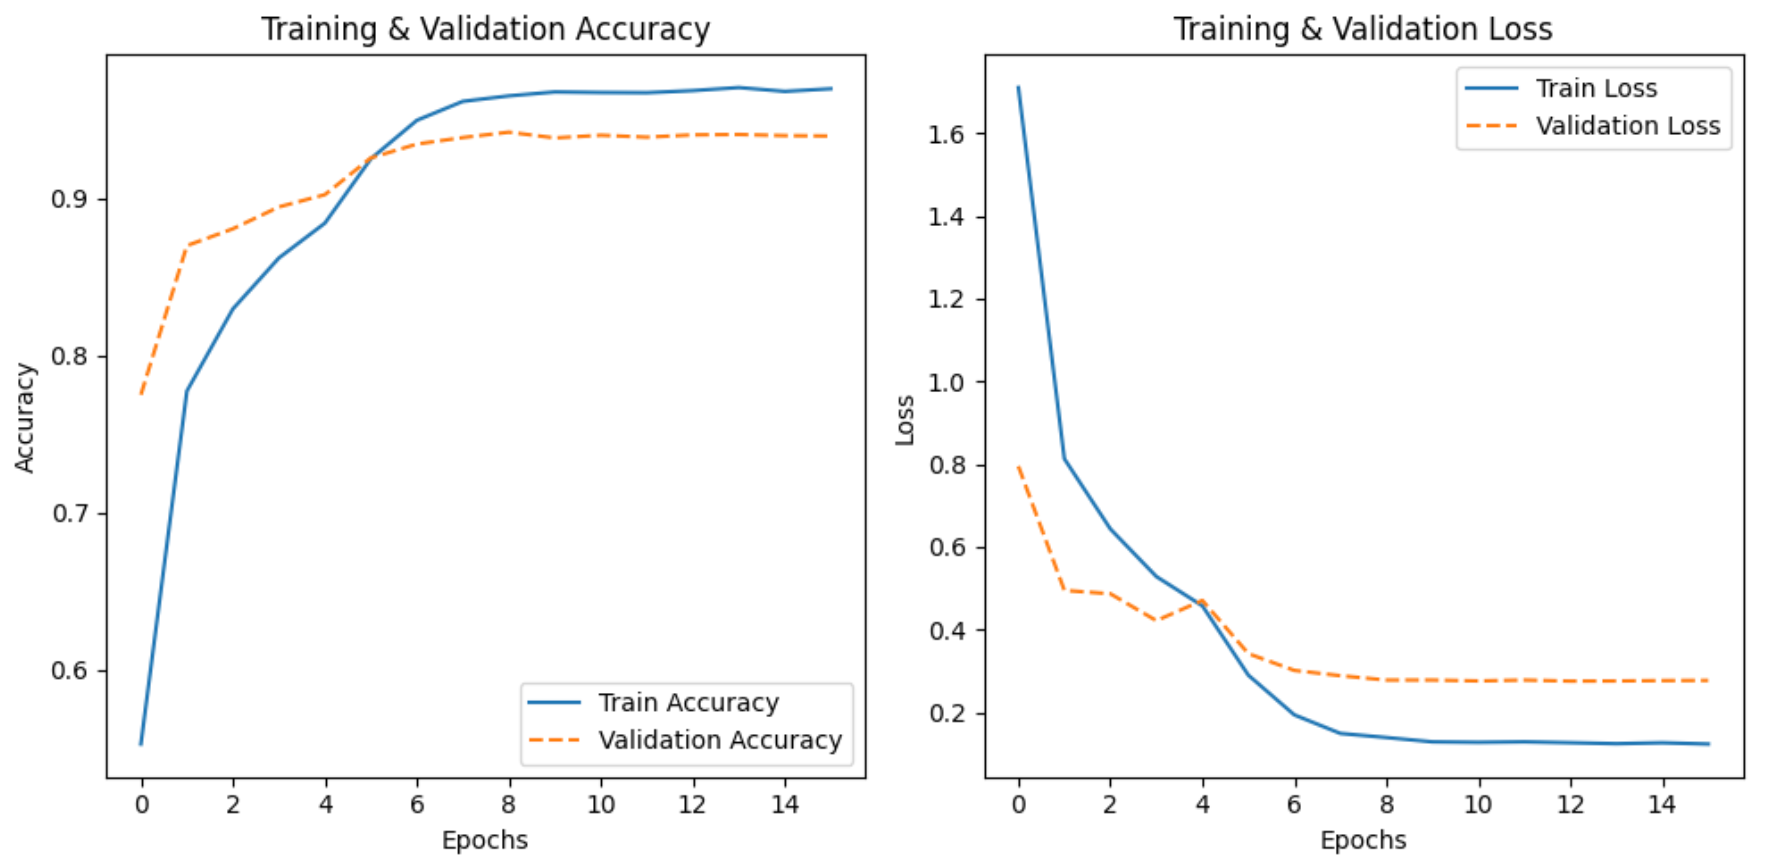
\includegraphics[scale=0.2]{images/GA_EfficientNet1.png}
      \caption{Accuracy and Loss for EfficientNetB3 in generation 1}
\end{figure}
\begin{figure}[htbp]
      \centering
      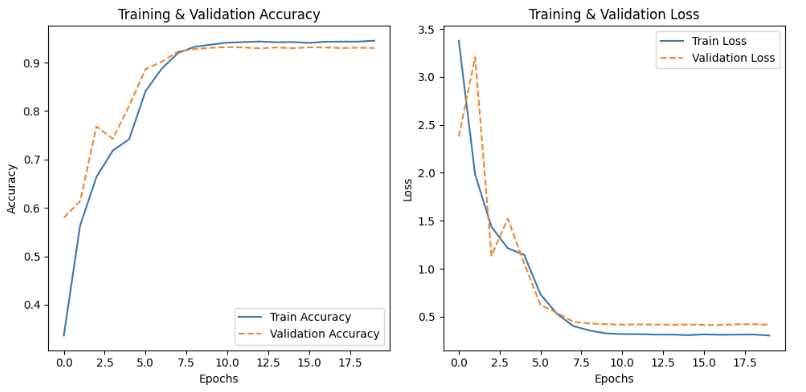
\includegraphics[scale=0.9]{images/GA_EfficientNet2.png}
      \caption{Accuracy and Loss for EfficientNetB3 in generation 2}
\end{figure}
\begin{figure}[htbp]
      \centering
      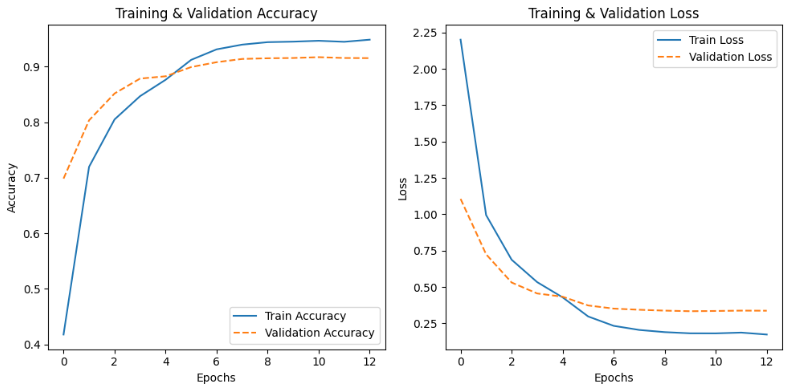
\includegraphics[scale=0.45]{images/GA_EfficientNet3.png}
      \caption{Accuracy and Loss for EfficientNetB3 in generation 3}
\end{figure}
\begin{figure}[htbp]
      \centering
      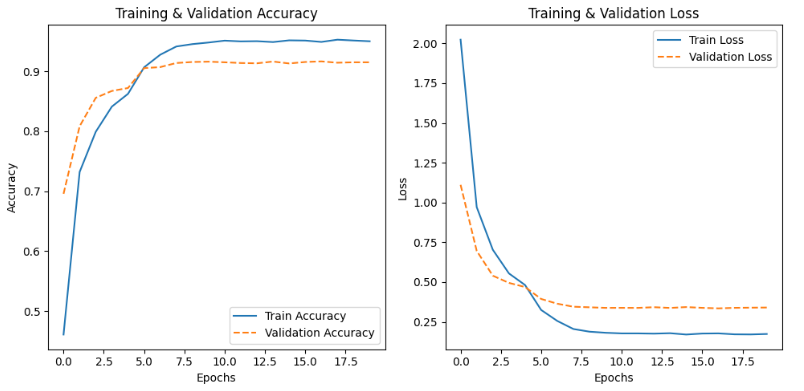
\includegraphics[scale=0.45]{images/GA_EfficientNet4.png}
      \caption{Accuracy and Loss for EfficientNetB3 in generation 4}
\end{figure}
\begin{figure}[htbp]
      \centering
      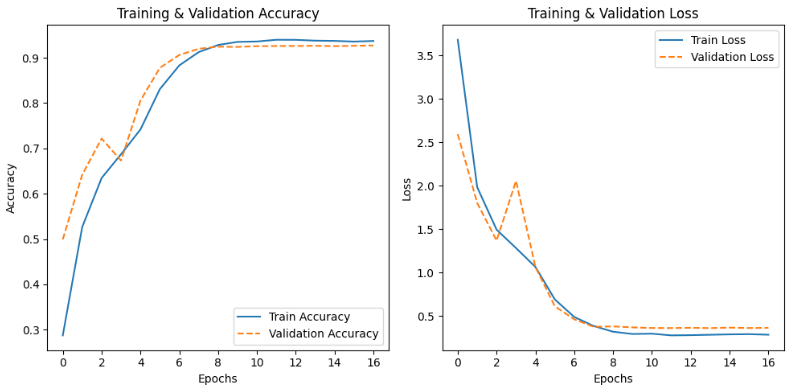
\includegraphics[scale=0.45]{images/GA_EfficientNet5.png}
      \caption{Accuracy and Loss for EfficientNetB3 in generation 5}
\end{figure}

\clearpage  % Ensures all figures are placed before proceeding to the table

The following table demonstrates different hyperparameter configurations and their corresponding test accuracies.

\begin{table}[h!]
      \centering
      \begin{tabular}{|c|c|c|c|c|c|c|c|}
          \hline
          \textbf{SN} & 
          \textbf{Batch} & \textbf{Img Size} & \textbf{LR} & \textbf{Epochs} & \textbf{Dropout} & \textbf{L2} & \textbf{Test Accuracy (\%)} \\
          \hline
          1 & 8   & 224x224 & 0.0001  & 20  & 0.2  & 1e-4  & \textbf{93.37} \\
          2 & 8   & 128x128 & 0.001   & 20  & 0.4  & 1e-4  & 92.54 \\
          3 & 16  & 128x128 & 0.0001  & 20  & 0.3  & 1e-4  & 90.68 \\
          4 & 8   & 128x128 & 0.0001  & 20  & 0.2  & 1e-4  & 91.02 \\
          5 & 8   & 128x128 & 0.001   & 20  & 0.2  & 1e-4  & 92.54 \\
          \hline
      \end{tabular}
      \caption{Hyperparameter configurations for Efficient-NetB3}
\end{table}

  
  
\subsubsection{Conclusion}
The best model achieved a Test Accuracy of \textbf{93.37\%} with a \textbf{Batch Size of 8}, \textbf{Image Size of 224x224}, \textbf{Learning Rate of 0.0001}, \textbf{Epochs = 20}, \textbf{Dropout Rate of 0.2}, and \textbf{L2 Regularization = 1e-4}. These results highlight the effectiveness of the Genetic Algorithm in systematically optimizing hyperparameters, leading to improved model performance and reduced overfitting.

% Figure
% \begin{figure}[h!]
%     \centering
%     \includegraphics[scale=0.18]{images/.png}
%     \caption{GA Efficient-Net.}
% \end{figure}

% Results

% Mobile Application    
\section{Mobile Application}
The mobile application allows the user to record the audio, visualize it with
waveforms during recording, before sending the actual audio data to the server
for processing. The user can also use the application to add their current
location to the map.The homepage of the application allows the user to view the birds along with 
the audio that are available in FeatherFind's database.
\begin{figure}[h!]
    \centering
    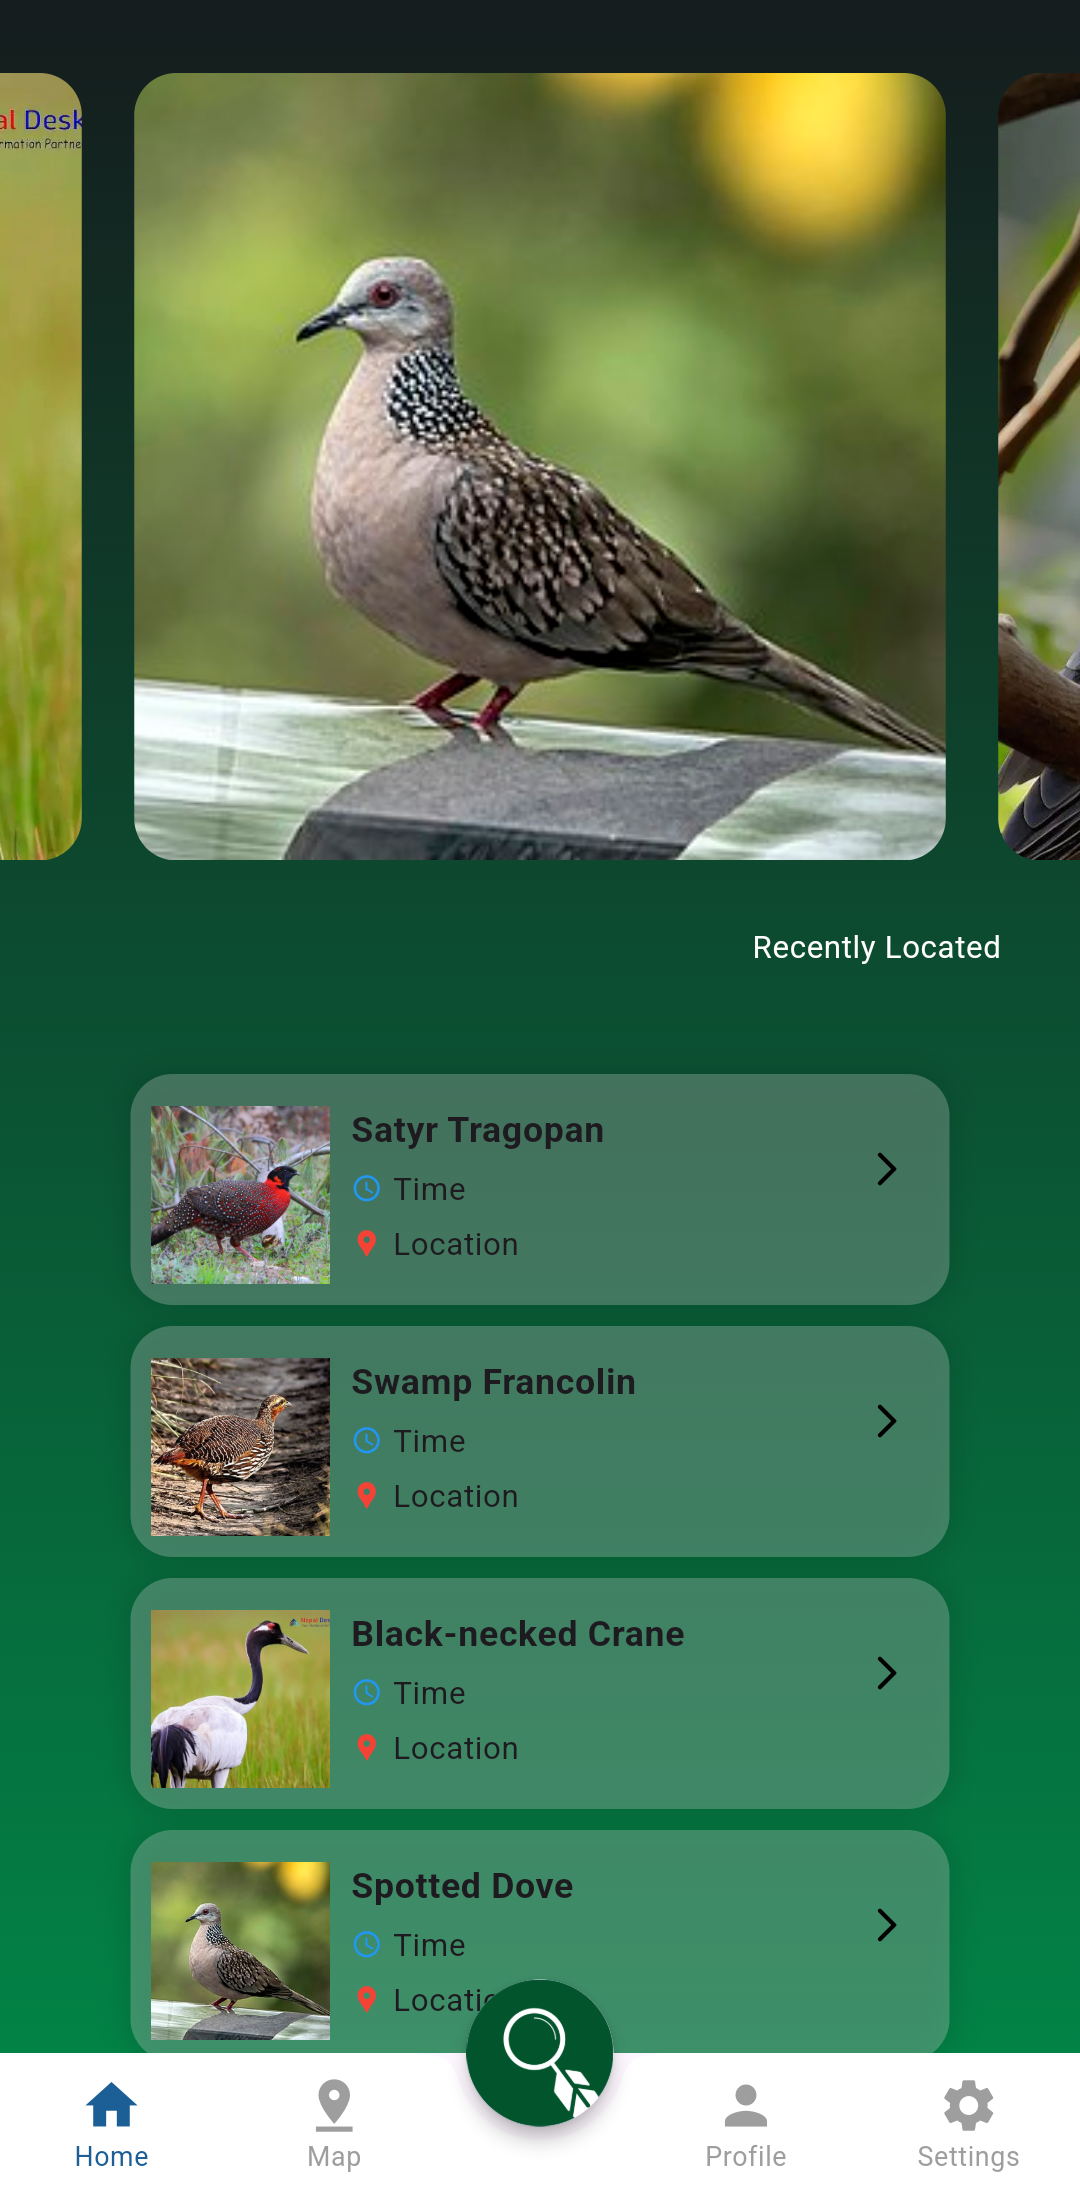
\includegraphics[scale=0.18]{images/Homepage.png}
    \caption{Home Page of FeatherFind.}
\end{figure}
The map page in FeatherFind allows the user to view all the birds that has been located
using the application and view their location in the maps embedded in the application alone 
with the detailed description of the birds.
\begin{figure}[h!]
    \centering
    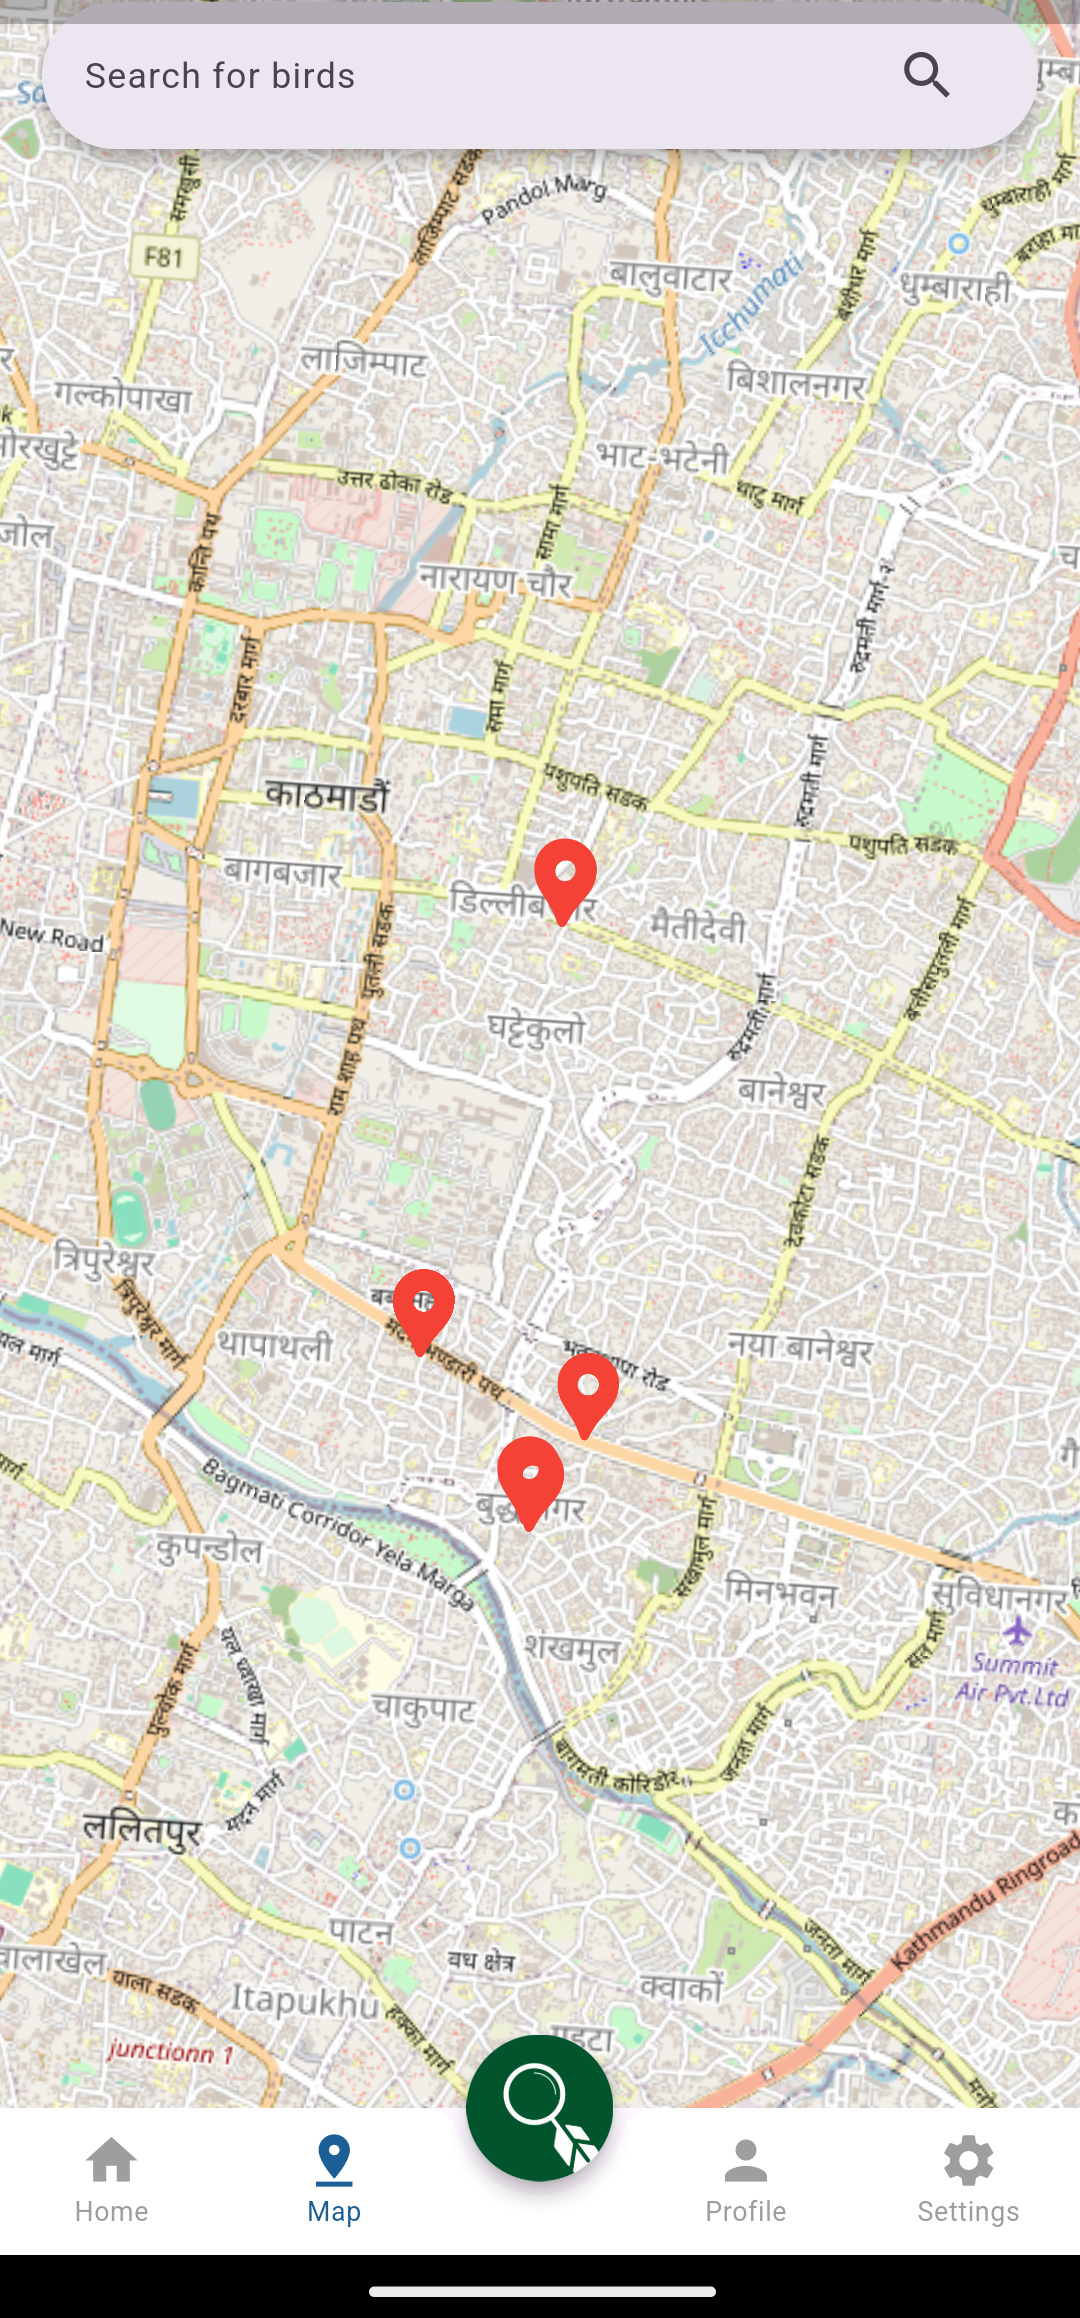
\includegraphics[scale=0.18]{images/mappage.png}
    \caption{Mapped Birds in FeatherFind.}
\end{figure}

For the audio recognition the user can record the audio in the application and as the 
audio is being recorded the app visualizes the audio in appropriate waveform. When the user stops
recording the audio, the user is prompted with a confirmation dialog, which can be used to process the 
audio and recognize it.
\begin{figure}[h!]
    \centering
    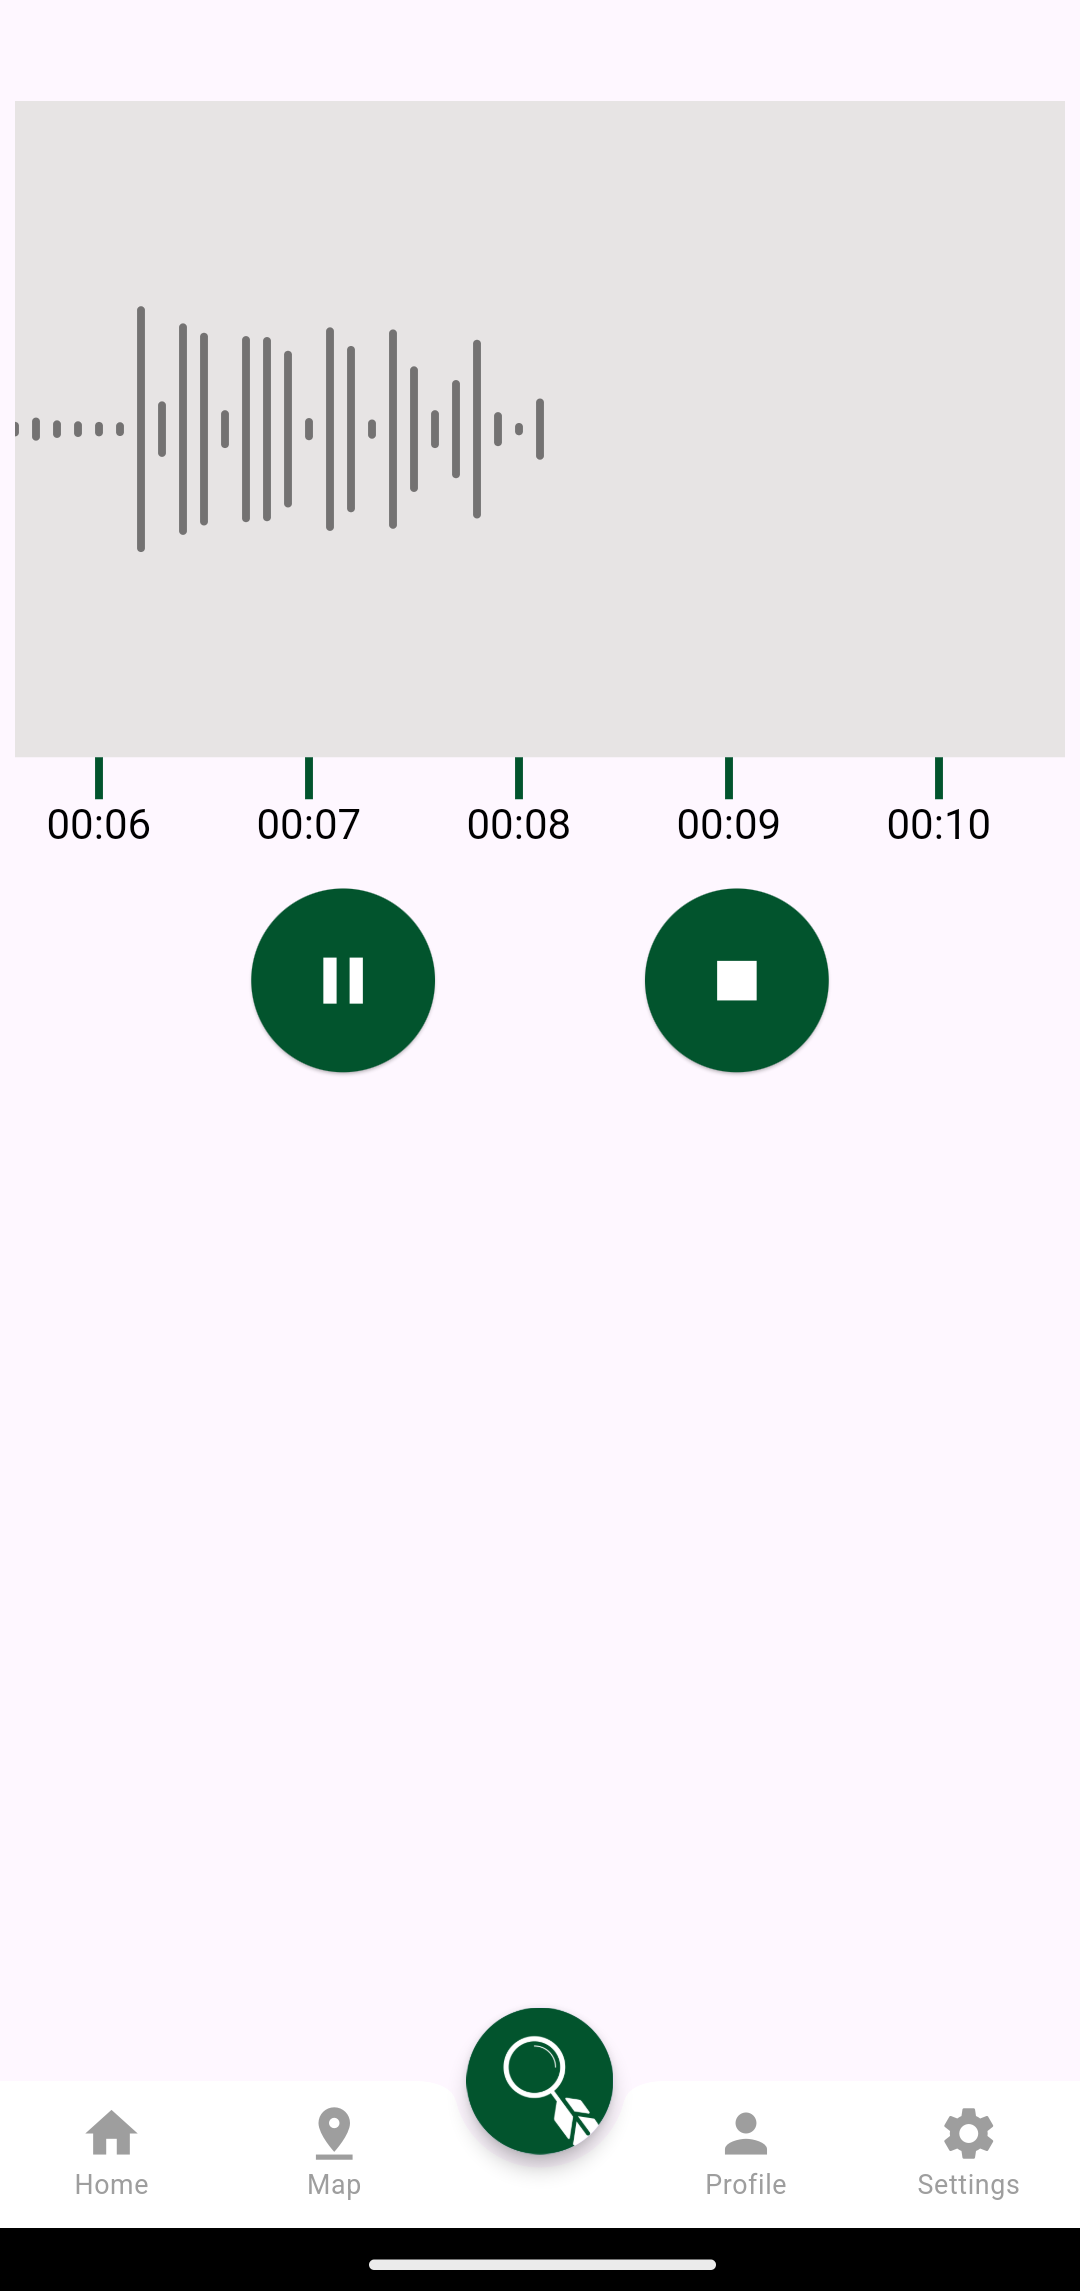
\includegraphics[scale=0.18]{images/recording.png}
    \caption{Recording using FeatherFind.}
\end{figure}

\begin{figure}[h!]
    \centering
    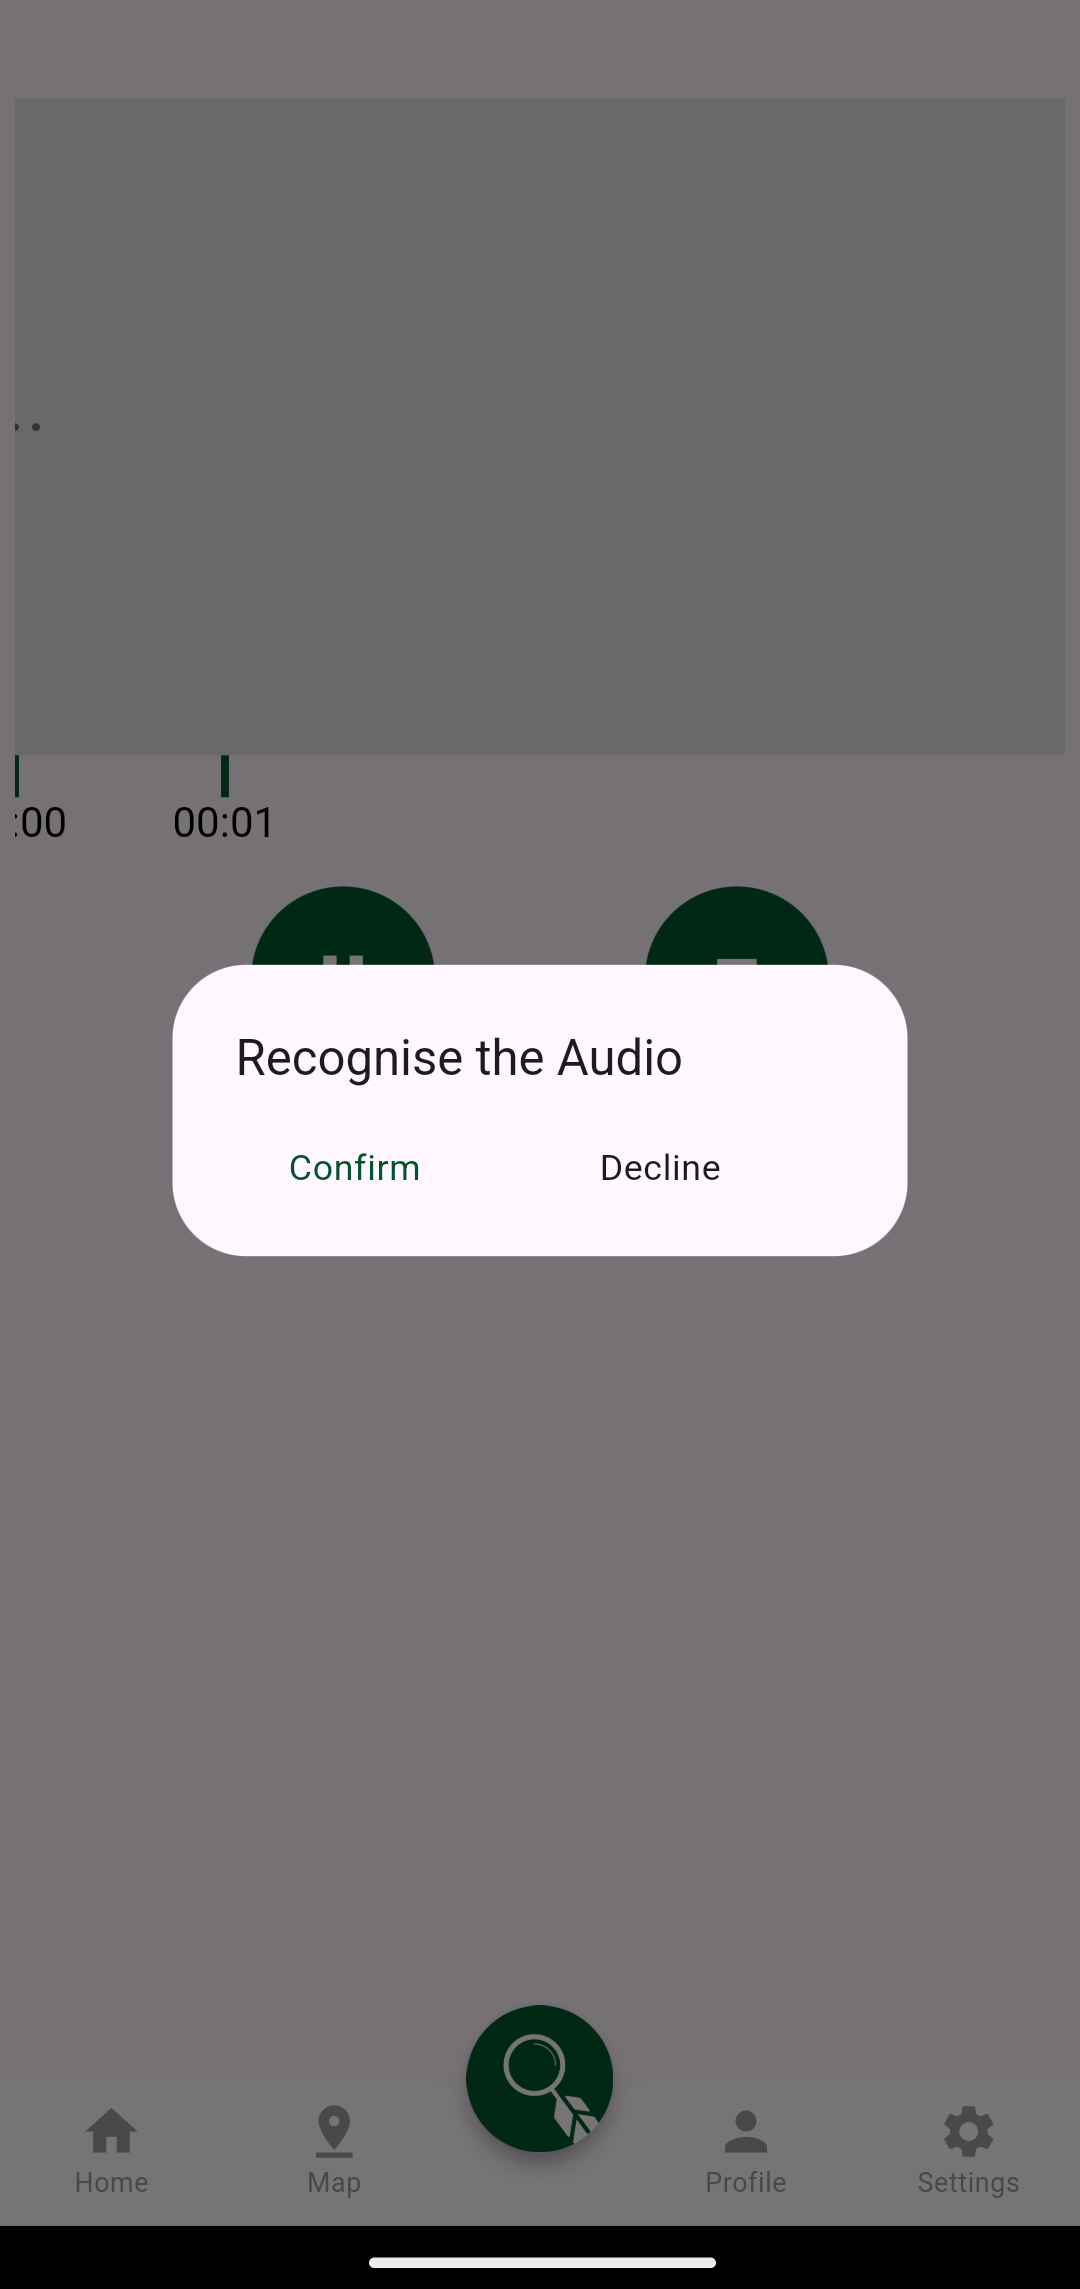
\includegraphics[scale=0.18]{images/confirmation.png}
    \caption{Confirmation for Audio Recognition.}
\end{figure}
\begin{figure}[h!]
    \centering
    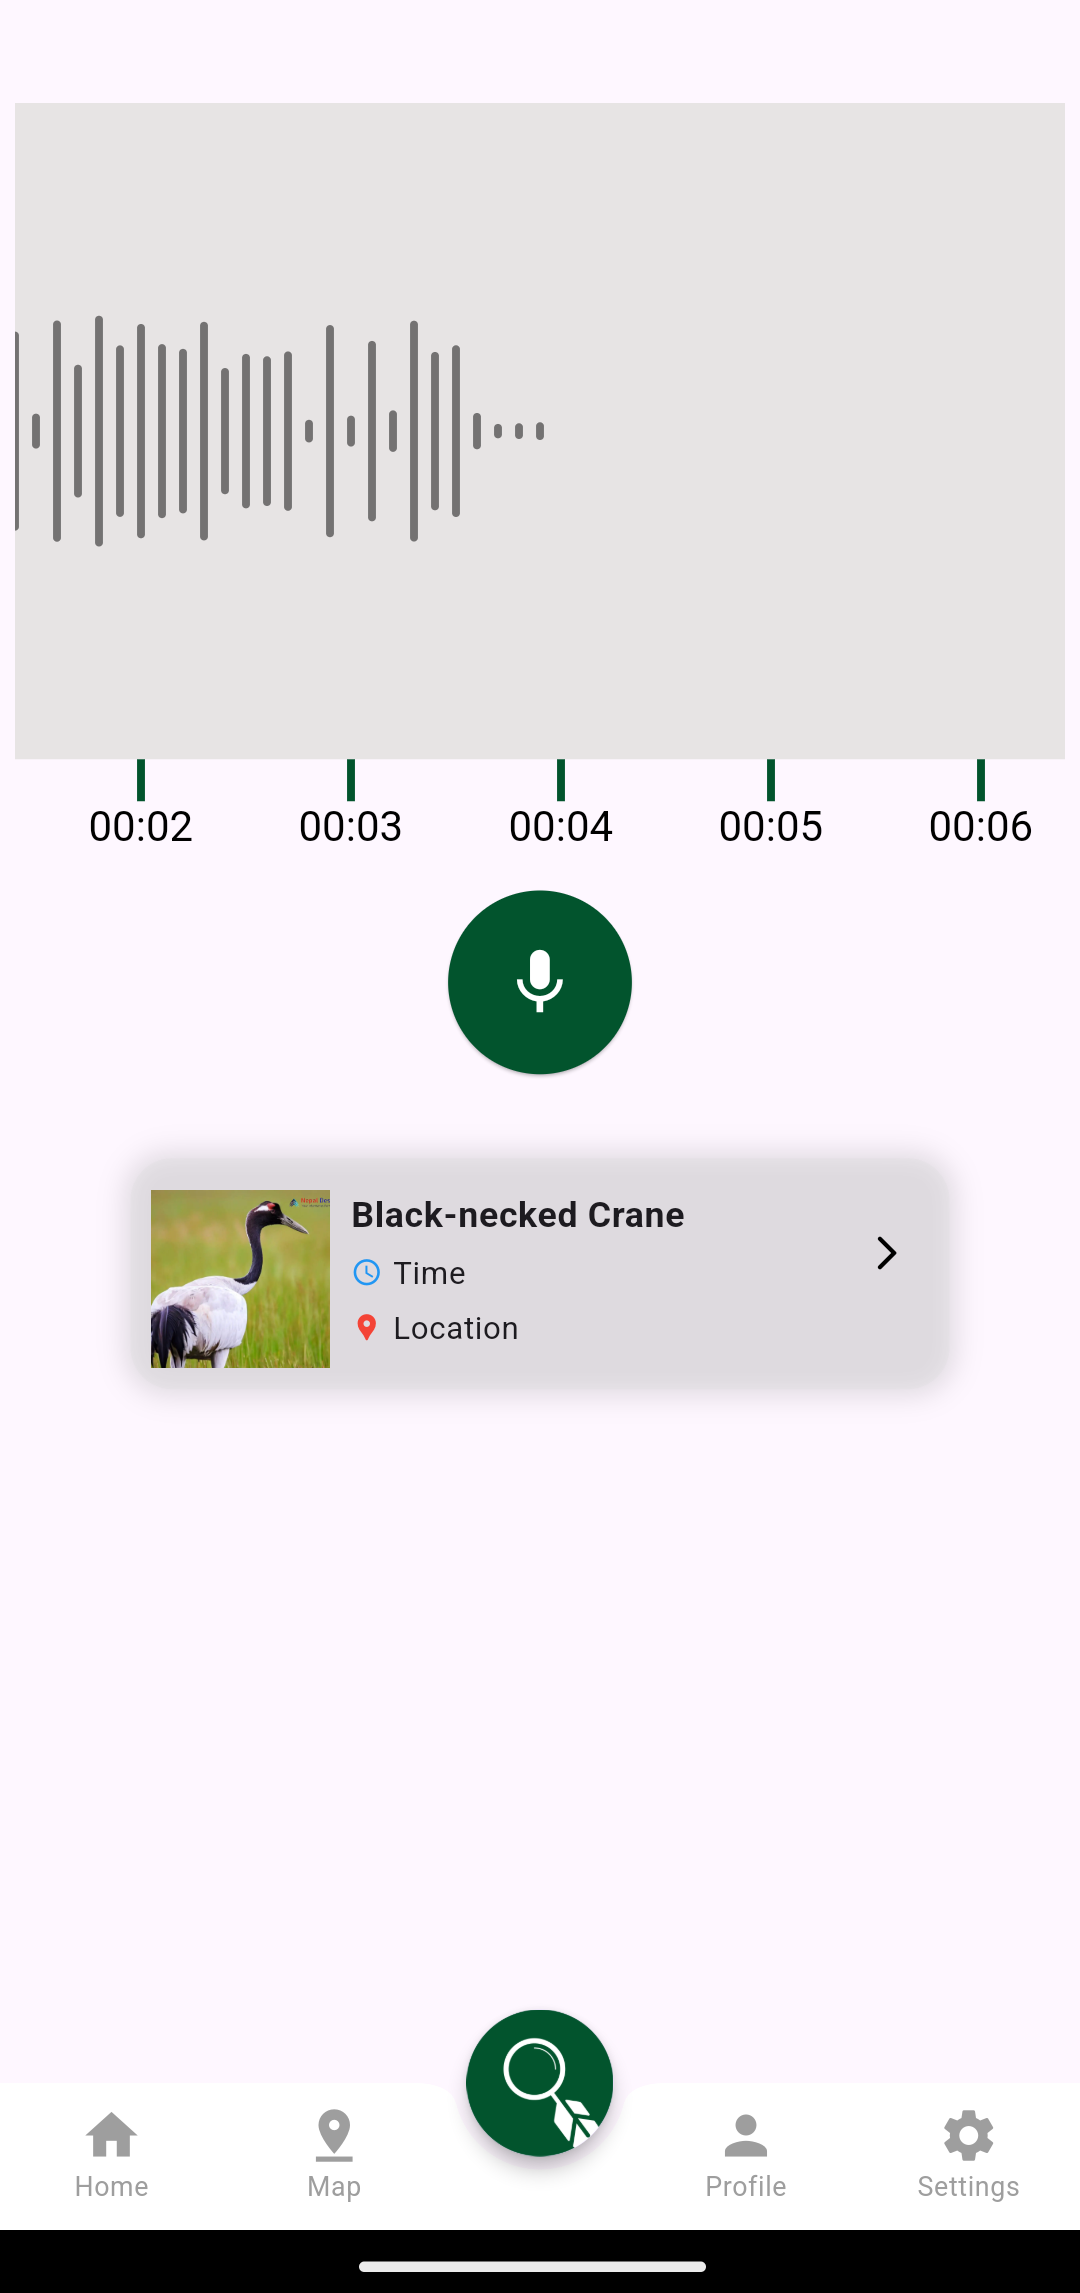
\includegraphics[scale=0.18]{images/Identified.png}
    \caption{Bird Species Identification using FeatherFind.}
\end{figure}


\newpage

\chapter{Discussion}
The FeatherFind project has made significant progress in developing an advanced
species identification using audio recordings.Some the key achievements of the
project include:
\section{Achievements}
\begin{itemize}
    \item Comprehensive Data Collection: The project successfully comiled an extensive
          dataset of d sounds by scraping Xeno-Canto, ensuring diversity in species
          representaion.
    \item Advanced Data Processing Techniques: The project utilized advancd audio
          processing techniques along with data augmentaion(time stretching,phase
          shifting, gradient noiise addition), were implemented to balance dataset and
          enhance model robustness.
    \item Feature Extraction and Model Training: Spectrograms and Mel-Frequency Cepstral
          Coefficients (MFCCs) were employed for feature extraction. EfficientNetB3
          architecture was utilized for bird species classification, achieving an
          accuracy of 89.36\% on the test dataset. Avolutional Neural Network (CNN)
          combined with Long ShoTerm Memory (LSTM) networks was used to capture both
          spatial ad temporal features.
    \item Genetic Algorithm for Hyperparameter Optimization: The model's performance was
          fine-tuned using genetic algorithms, ensuring optimal parameter selection for
          improved accuracy.
    \item Bird Sound Detection Model: A preliminary model was trained to verify the
          presence of bird sounds before classification, using the InceptionV3
          network.AUC score of 83\% and an accuracy of 87.28\% was achieved.
    \item Deployment and Mobile App Development: The classification model was deployed on
          Huggingface Spaces for seamless API integration.A mobile application was
          developed to allow users to record and analyze bird sounds in real-time while
          tagging locations using GPS integration.
\end{itemize}

\section{Limitations}
\begin{itemize}
      \item Dataset limitations : Since the dataset lacks sufficient variation in bird species, 
      environmental noise, and recording conditions, FeatherFind struggles with real-world scenarios. 
      Additionally, because certain bird species are overrepresented, the model produces biased predictions, 
      making it less reliable for species with fewer training samples.
      \item Multiple bird sound : Since the system is optimized to recognize only a single dominant bird call in an audio recording, 
      it fails to accurately identify multiple birds vocalizing simultaneously. When overlapping sounds occur, the model either 
      misclassifies them or ignores background calls, limiting its ability to handle complex audio environments.
      \item
\end{itemize}
  
\section{Future Improvements}

%Reference
\renewcommand\bibname{REFERENCES} % Change heading to References
\bibliographystyle{IEEEtran} % to use IEEE Format for referencing
\addcontentsline{toc}{chapter}{References} % to add references in TOC
\bibliography{library} % specify the .bib file containing reference information 

%Comment this Chapter if you do not need to include Appendix.

%\addcontentsline{toc}{chapter}{Appendix}

\end{document}
